This chapter provides a comprehensive technical description of the \GRust language. It begins with a
practical example to illustrate core concepts, then delves into the specification of the syntax,
identifier usage, and type system. The chapter subsequently details the implementation of the
prototype compiler, explaining its architecture and compilation pipelines. Finally, it presents
benchmarks that validate the performance, expressiveness, and industrial applicability of the
language.

The chapter is structured as follows.
\begin{description}
    \item[\Cref{sec:grust:example}]
          presents an Adaptive Cruise Control (ACC) example to showcase the main features of \GRust.
          It demonstrates how to model services with the \GRFRP kernel, define stateful components
          with the \GRSync kernel, and specify safety properties for formal verification with
          \GReusot.

    \item[\Cref{sec:grust:syntax}]
          presents the language syntax using EBNF notation. This covers the asynchronous \GRFRP
          kernel for service modeling, the \GReact library of built-in operators, the synchronous
          \GRSync kernel for component definition, and the \GReusot extension for formal contracts.

    \item[\Cref{sec:grust:id_usage}]
          formalizes the rules for identifier usage with inference rules that define scoping
          mechanisms for the language, including the sequential, lexical scoping of \GRFRP services
          and the mutually recursive scoping of \GRSync components.

    \item[\Cref{sec:grust:typing}]
          details the static type system, which ensures the correct composition of synchronous and
          asynchronous constructs. It distinguishes between \emph{flow types} (\eg \texttt{signal},
          \texttt{event}) and \emph{sampling types} (\eg \texttt{type}, \texttt{type?}).

    \item[\Cref{sec:grust:implem}]
          describes the implementation of the prototype compiler, including its architecture as a
          \Rust procedural macro. It details the compilation pipelines for both sub-languages:
          \GRSync components are compiled into synchronous state machines, and \GRFRP services into
          asynchronous data-propagation machines. The translation of \GReusot specifications into
          \Creusot annotations is also explained.

    \item[\Cref{sec:grust:benchmarks}]
          concludes with a three-part benchmark evaluation. A quantitative analysis compares the
          performance of generated code against established \Lustre compilers. A qualitative case
          study on a UAV Kalman filter demonstrates improved design clarity over a \Ci
          implementation. Finally, an industrial evaluation at \ampere shows significant code
          reduction and equivalent performance when reimplementing production services in \GRust.
\end{description}

\section{Example: Adaptive Cruise Control (ACC)}
\label{sec:grust:example}

This section introduces the \GRust language through an Adaptive Cruise Control (ACC) example, a
common feature in Advanced Driver-Assistance Systems (ADAS). The full program is listed in
\Cref{fig:code_acc} and can be found as a running example in the \GRust repository at
\begin{center}
  \url{https://github.com/langrust/grust/tree/main/examples/acc}.
\end{center} When active, the ACC system computes
the braking force required to maintain a safe distance from a preceding vehicle, based on the
current speed and the measured distance.

\begin{figure}[ht!]
  \begin{lstlisting}[
      language=GRust,
      caption={[\GRust program for the Adaptive Cruise Control example.]%
      Example of a \GRust program for an Adaptive Cruise Control system.},
      captionpos=b,
      label={fig:code_acc}
  ]
  // Interface to the broader car system
  import signal car::state::speed_km_h        : float; $\label{line:grust:example:interface:begin}$
  import signal car::sensors::radar_m         : float;
  import event  car::hmi::acc_active          : Activation;
  import event  car::core::derive             : unit; $\label{line:grust:example:import:end}$
  export signal car::actuators::brakes_m_s    : float; $\label{line:grust:example:interface:end}$
  // Activation type
  enum Activation { Off, On }
  // Adaptive Cruise Control service
  service adaptive_cruise_control @[10, 3000] { $\label{line:grust:example:acc_service:begin}$
    let event  radar_e: float = on_change(radar_m); $\label{line:grust:example:on_change}$
    let signal cond: bool = activate(acc_active, radar_e); $\label{line:grust:example:cond}$
    let signal speed_m_s: float = convert(speed_km_h); $\label{line:grust:example:speed_m_s}$
    let signal delta_v: float = derive_on(radar_m, time(), derive); $\label{line:grust:example:delta_v}$
    brakes_m_s = acc(cond, radar_m, speed_m_s, delta_v); $\label{line:grust:example:brakes_m_s}$
  } $\label{line:grust:example:acc_service:end}$
  // Filters the ACC on driver activation and when approaching FV
  component acc(c: bool, d: float, s: float, v: float) -> (b: float) { $\label{line:grust:example:acc:begin}$
    match c {
      true  => { b = v^2 / (2. * (d - d_safe));
                 let d_safe: float = safety_distance(s, fv_v);
                 let fv_v: float = s + v; }
      false => { b = 0.; let (fv_v: float, d_safe: float) = (0., 0.); }
    }
  } $\label{line:grust:example:acc:end}$
  // Activation condition of the ACC
  component activate(act: Activation?, r: float?) -> (c: bool) { $\label{line:grust:example:activate:begin}$
    when { $\label{line:grust:example:when:begin}$
      init => { r_mem = 0.; active = false; approach = false; } $\label{line:grust:example:when:init}$
      act? => { let active: bool = act == Activation::On; } $\label{line:grust:example:when:act}$
      r?   => { let r_mem: float = r; let approach: bool = r < last r_mem; } $\label{line:grust:example:declaration}$
    }
    c = active && approach; $\label{line:grust:example:assignments}$
  } $\label{line:grust:example:activate:end}$
  // Derive on a specific event `e`.
  component derive_on(x: float, t: float, e: unit?) -> (v: float) { $\label{line:grust:example:derive_on:begin}$
    when {
      init => { v = 0.; x_mem = 0.; t_mem = 0.; }
      e?   => { v = 1000. * (x - last x_mem) / (t - last t_mem);
                let (x_mem: float, t_mem: float) = (x, t); }
    }
  } $\label{line:grust:example:derive_on:end}$
  // Safety distance computation
  function safety_distance(sv_v: float, fv_v: float) -> float { $\label{line:grust:example:safety_distance:begin}$
    let (rho: float, b_max: float) = (1., 0.6*9.81);
    let sv_d_stop: float = sv_v*rho + sv_v^2/(2.*b_max);
    let fv_d_stop: float = fv_v^2/(2.*b_max);
    return sv_d_stop - fv_d_stop;
  } $\label{line:grust:example:safety_distance:end}$
  \end{lstlisting}
\end{figure}

\subsection{Syntax}

The \GRust language is composed of three core elements, which we will describe using
the ACC example from \Cref{fig:code_acc}: the \GRFRP kernel for modeling services,
the \GReact library of built-in operators, and the \GRSync kernel for defining
synchronous components.

\paragraph{Service-modeling kernel (\GRFRP)}
In \GRust, the primary unit of organization is the \emph{service}, an entity that
computes data flows and connects to the rest of the system through the definition of an
\emph{interface}. Both are modeled in \GRFRP, where flows are categorized as
\emph{signals} for values that evolve over time, and \emph{events} for discrete,
punctual occurrences.

The example defines the \texttt{adaptive\_cruise\_control} service
(\Crefrange{line:grust:example:acc_service:begin}{line:grust:example:acc_service:end}).
Its interface
(\Crefrange{line:grust:example:interface:begin}{line:grust:example:interface:end})
declares the flows it consumes and produces.
%
The imported flows
(\Crefrange{line:grust:example:interface:begin}{line:grust:example:import:end})
are inputs from the system, including the vehicle speed (\texttt{speed\_km\_h}) and
radar distance (\texttt{radar\_m}) as signals, and the driver's command
(\texttt{acc\_active}) and an internal trigger (\texttt{derive}) as events.
%
The computed braking force (\texttt{brakes\_m\_s}) is exported as a signal for use by
actuators (\Cref{line:grust:example:interface:end}).
%
The service body defines its logic by declaring local flows in a declarative style
(\Crefrange{line:grust:example:on_change}{line:grust:example:delta_v}). These include
\texttt{radar\_e}, an event fired when the radar distance changes; \texttt{cond}, a
signal representing the activation condition; \texttt{speed\_m\_s}, the converted
vehicle speed; and \texttt{delta\_v}, the relative speed to the front vehicle.

\paragraph{Built-in reactive library (\GReact)}
The logic within a service is constructed by composing flow operators. \GRust
provides a standard library of built-in operators called \GReact. In the ACC
example, the service uses two such operators: \texttt{on\_change}
(\Cref{line:grust:example:on_change}), which takes the \texttt{radar\_m} signal and
produces the \texttt{radar\_e} event whenever the signal's value changes; and
\texttt{time} (\Cref{line:grust:example:delta_v}), which provides a signal
representing the current execution time.

\paragraph{Component-modeling kernel (\GRSync)}
Beyond built-in operators, services can use custom, user-defined operators called
\emph{components}. The ACC service uses four components: \texttt{activate},
\texttt{convert}, \texttt{derive\_on}, and \texttt{acc}
(\Crefrange{line:grust:example:cond}{line:grust:example:brakes_m_s}). The definitions
for the stateful components are provided in the code listing
(\Crefrange{line:grust:example:acc:begin}{line:grust:example:derive_on:end}).

Components are defined in \GRSync, a synchronous language where computation proceeds
in discrete logical instants. At each instant, a component computes its output values
based on the values of its inputs at that same instant. Input events, which may not
be present in every step, are represented by optional types, indicated with a question
mark (\eg \texttt{Activation?} in \Cref{line:grust:example:activate:begin}).

The logic of a component is specified by a set of unordered equations that are
evaluated synchronously. The \texttt{activate} component, for instance, uses several
kinds of equations to define its output \texttt{c}
(\Crefrange{line:grust:example:when:begin}{line:grust:example:assignments}):
\begin{itemize}
  \item \emph{Standard equations} define values through simple assignments, such as
        \texttt{c = active \&\& approach;} (\Cref{line:grust:example:assignments}),
        or local declarations, like \texttt{let r\_mem: float = r;}
        (\Cref{line:grust:example:declaration}).
  \item \emph{\texttt{when} equations} activate computations only on discrete
        occurrences, such as an event's arrival. This construct is reminiscent of a
        state machine's transition system. It can define initial values for state
        variables (\Cref{line:grust:example:when:init}) and update them when a
        specific event is present, such as \texttt{act?}
        (\Cref{line:grust:example:when:act}).
  \item \emph{\texttt{match} equations} select a computational branch based on a
        signal's value. Unlike \texttt{when}, \texttt{match} patterns must be
        exhaustive, ensuring a branch is always executed. This is analogous to the
        state definitions in a state machine.
\end{itemize}

Components can maintain internal state across instants by using the \texttt{last}
keyword, which accesses a value from the previous step. For example, in the
\texttt{activate} component, \texttt{r < last r\_mem}
(\Cref{line:grust:example:declaration}) compares the current radar value with the
one from the previous step where \texttt{r} was present. For purely combinatorial
logic, \GRust also provides memory-less \emph{functions} like
\texttt{safety\_distance}
(\Crefrange{line:grust:example:safety_distance:begin}{line:grust:example:safety_distance:end}),
which use ordered equations and cannot hold state.

\subsection{Execution}

The execution of the ACC service, illustrated in \Cref{fig:execution_acc}, follows a
dataflow model. It propagates signal changes and event occurrences through the network
of operators defined in the service. All incoming flows are timestamped. The
\texttt{time} operator obtains its values from these timestamps (orange arrows in the
diagram). A context maintains the most recent value of signals such as
\texttt{speed\_m\_s}, \texttt{cond}, \texttt{radar\_m}, and \texttt{delta\_v}, making
them available for components to read at any time.

\begin{figure}[!ht]
  \centering
  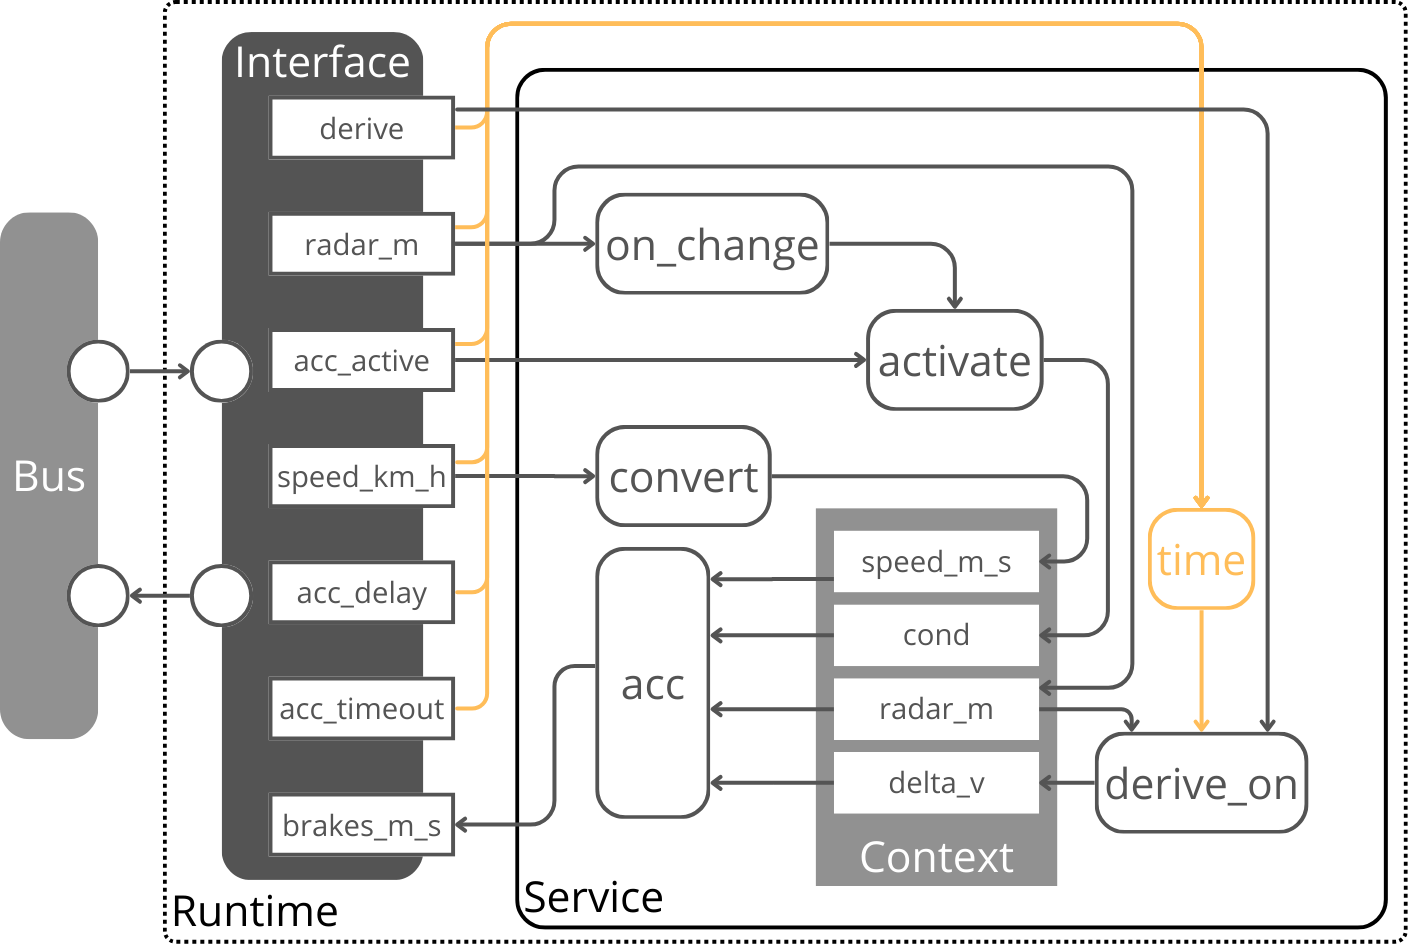
\includegraphics[width=0.7\textwidth]{../images/execution_acc.png}
  \caption[Adaptive Cruise Control execution.]%
  {Execution schematic for the Adaptive Cruise Control service from
    \Cref{fig:code_acc}.}
  \label{fig:execution_acc}
\end{figure}

Here is an example of propagation.
When \texttt{speed\_km\_h} changes, it triggers the \texttt{convert} component, which
updates \texttt{speed\_m\_s} in the context. Concurrently, the timestamp updates the
\texttt{time()} signal, which in turn triggers \texttt{derive\_on}. The
\texttt{derive\_on} component retrieves the value of the signal \texttt{radar\_m} from
the context and computes the updated value of \texttt{delta\_v}. Once
\texttt{speed\_m\_s} and \texttt{delta\_v} are updated, they propagate to the
\texttt{acc} component, ensuring that all its inputs are up to date. If one of its
inputs has changed, the \texttt{acc} component then computes the current value of
\texttt{brakes\_m\_s}. Finally, the value of \texttt{brakes\_m\_s} is sent through the
bus, only if it has changed.

To prevent both excessive updates and long periods without output, the service adheres
to timing constraints specified by \texttt{@[10, 3000]}
(\Cref{line:grust:example:acc_service:begin}). This annotation ensures that outputs are
produced at most every 10~ms and at least every 3000~ms. If inputs arrive faster than
the 10~ms minimum delay, they are buffered. These timing events are represented in
\Cref{fig:execution_acc} as \texttt{acc\_delay} and \texttt{acc\_timeout}. The
buffering mechanism is omitted from the diagram for clarity.


\begin{table}[ht!]
  \centering
  \begin{tabular}{l|ccccccccc}
    timestamp                 & {$t$}                 & {$t + 5$}      & {$t + 10$}         & {$t + 25$}         & {$t + 40$}         & {$t + 525$}         & {$t + 650$}         \\ \hline
    \verb|speed_km_h|         & 129.                  & \changed{131.} & \stored{131.}      & 131.               & 131.               & 131.                & \changed{128.}      \\
    \verb|radar_m|            & 130.                  & 130.           & 130.               & 130.               & \changed{125.}     & 125.                & 125.                \\
    \verb|acc_active|         & \changed{\texttt{On}} &                &                    &                    &                    &                     &                     \\
    \verb|derive|             &                       &                &                    & \changed{()}       &                    & \changed{()}        &                     \\
    \local{\texttt{x\_mem}}   & \local{130.}          & \local{$\bot$} & \local{130.}       & \local{130.}       & \local{130.}       & \local{125.}        & \local{125.}        \\
    \verb|time|               & \updated{$t$}         & $t$            & \updated{$t + 10$} & \updated{$t + 25$} & \updated{$t + 40$} & \updated{$t + 525$} & \updated{$t + 650$} \\
    \verb|delta_v|            & 0.                    & 0.             & 0.                 & 0.                 & 0.                 & \updated{-10.}      & -10                 \\
    \verb|radar_e|            &                       &                &                    &                    & \updated{125.}     &                     &                     \\
    \local{\texttt{active}}   & \local{true}          & \local{$\bot$} & \local{$\bot$}     & \local{$\bot$}     & \local{true}       & \local{$\bot$}      & \local{$\bot$}      \\
    \local{\texttt{r\_mem}}   & \local{130.}          & \local{$\bot$} & \local{$\bot$}     & \local{$\bot$}     & \local{125.}       & \local{$\bot$}      & \local{$\bot$}      \\
    \local{\texttt{approach}} & \local{false}         & \local{$\bot$} & \local{$\bot$}     & \local{$\bot$}     & \local{true}       & \local{$\bot$}      & \local{$\bot$}      \\
    \verb|cond|               & false                 & false          & false              & false              & \updated{true}     & true                & true                \\
    \verb|speed_m_s|          & 35.8                  & 35.8           & \updated{36.4}     & 36.4               & 36.4               & 36.4                & \updated{35.6}      \\
    \local{\texttt{fv\_v}}    & \local{$\bot$}        & \local{$\bot$} & \local{0.}         & \local{$\bot$}     & \local{36.4}       & \local{26.4}        & \local{25.6}        \\
    \local{\texttt{d\_safe}}  & \local{$\bot$}        & \local{$\bot$} & \local{0.}         & \local{$\bot$}     & \local{36.4}       & \local{89.7}        & \local{87.5}        \\
    \verb|brakes_m_s|         & 0.                    & 0.             & 0.                 & 0.                 & 0.                 & \updated{1.4}       & \updated{1.3}
  \end{tabular}
  \caption[Chronogram of an execution for the Adaptive Cruise Control.]%
  {Example chronogram for an execution of the ACC service from \Cref{fig:code_acc}.
    The legend for colors is: \changed{red} for input changes, \stored{green} for stored
    inputs, and \updated{blue} for local/exported flow updates. Internal component
    variables are in \local{gray}; \local{$\bot$} denotes absence of a value.
  }
  \label{fig:chronogram_acc}
\end{table}

\Cref{fig:chronogram_acc} shows an execution trace of the ACC service, which we can
follow step by step:
\begin{itemize}
  \item At time $t$, the driver activates the ACC, causing the \texttt{acc\_active} event to
        occur with the value \texttt{On}. This triggers the \texttt{activate} component, where
        the \texttt{act?} branch (\Cref{line:grust:example:when:act}) sets the internal state
        \texttt{active} to \texttt{true}. However, the \texttt{approach} state remains
        \texttt{false}, so the activation condition \texttt{cond} is \texttt{false}.
        Consequently, the output \texttt{brakes\_m\_s} remains at its initial value of 0.

  \item At $t+5$, a change in \texttt{speed\_km\_h} arrives. However, because the 10~ms minimum
        delay specified by \texttt{@[10, 3000]} (\Cref{line:grust:example:acc_service:begin})
        has not elapsed, the update is buffered and computation is deferred.

  \item At $t+10$, the minimum delay has passed, and the buffered input is processed. This
        triggers the \texttt{convert} component, updating \texttt{speed\_m\_s}. This change
        propagates to the \texttt{acc} component, but since \texttt{cond} is still
        \texttt{false}, the component's \texttt{match} statement
        (\Cref{line:grust:example:acc:begin}) takes the \texttt{false} branch, setting the
        braking force to 0 and leaving the output unchanged.

  \item At $t+25$, the \texttt{derive} event occurs, triggering the \texttt{derive\_on}
        component. Although a computation occurs, the resulting \texttt{delta\_v} is 0, so the
        output of \texttt{acc} remains unchanged.

  \item At $t+40$, the \texttt{radar\_m} signal changes from 130 to 125. This triggers the
        \texttt{on\_change} operator (\Cref{line:grust:example:on_change}), which emits the
        \texttt{radar\_e} event. In the \texttt{activate} component, the \texttt{r?} branch
        (\Cref{line:grust:example:declaration}) executes. Since the new radar value (125) is
        less than the previously stored one (130), the \texttt{approach} state becomes
        \texttt{true}. With both \texttt{active} and \texttt{approach} now being \texttt{true},
        the output \texttt{cond} becomes \texttt{true}. Although \texttt{acc} is now active,
        the braking force is still computed as zero because its input \texttt{delta\_v} is
        zero, so no new value is sent to the bus.

  \item At $t+525$, another \texttt{derive} event triggers \texttt{derive\_on}
        (\Cref{line:grust:example:derive_on:begin}). This time, using the previous radar and
        time values, \texttt{delta\_v} is updated to $-10$. This significant change in one of
        the inputs to \texttt{acc} causes it to recompute the braking force. With a non-zero
        relative speed, the \texttt{true} branch of the \texttt{match} statement now yields a
        braking force of $0.60$, which is sent to the bus.

  \item Finally, at $t+650$, a change in \texttt{speed\_km\_h} updates \texttt{speed\_m\_s}.
        This change again triggers the \texttt{acc} component, which re-evaluates its logic
        and outputs a new braking force of $0.57$.
\end{itemize}

\subsection{Verification}
\label{sec:grust:example:greusot}

The \iso standard governs functional safety for automotive systems, defining Automotive Safety
Integrity Levels (\Asil) from A (least critical) to D (most critical). Achieving compliance for
critical systems (\Asil~D) requires rigorous verification to prove the absence of faults like
arithmetic overflows or memory errors. Since runtime checks are often too costly for embedded
environments, this proof is typically done through static verification.

For an engineer, formal verification of traditional \Ci code imposes a significant burden. They must
manually prove fundamental memory safety properties, such as the absence of null pointer
dereferences, buffer overflows, or data races. This process is tedious and error-prone, consuming
effort that could be spent on verifying the functional logic of the system itself. In contrast,
\GRust generates \Rust code, a language whose design offers a distinct advantage for verification.
The \Rust compiler's borrow checker statically enforces memory and thread safety, eliminating entire
classes of bugs before the formal verification stage even begins.

This foundation allows a deductive verifier like \Creusot~ \cite{DBLP:conf/icfem/DenisJM22} to
streamline the proof process. From the user's perspective, the task shifts from proving low-level
memory correctness to specifying and proving high-level functional properties. An engineer annotates
their code with contracts---preconditions, postconditions, and invariants---that capture the
intended behavior. Verification is then performed by running \texttt{cargo creusot prove} on the
crate containing the generated code. \Creusot then attempts to prove that the implementation adheres
to these contracts.
%
By default, it also proves the absence of runtime panics, such as arithmetic overflows, providing a
strong baseline of safety automatically. For more advanced needs, engineers can add explicit
properties to verify critical system logic. To make these capabilities accessible at the modeling
level, we introduce \GReusot, a wrapper for the specification language of \Creusot that enables
verification of \GRSync components and functions.

\subsubsection{Specifying the ACC in \GReusot}
\label{sec:grust:example:greusot:acc}

\Cref{lst:grust:example:greusot:fun:spec,lst:grust:example:greusot:comp:spec} show the ACC example
extended with \GReusot specifications. Since \Creusot does not support
floating-point arithmetic, all values are represented as integers.

The specification for the \texttt{safety\_distance} function, shown in
\Cref{lst:grust:example:greusot:fun:spec}, defines its expected operating conditions. The
preconditions, specified in
\Cref{line:grust:example:greusot:fun:spec:sv_v,line:grust:example:greusot:fun:spec:fv_v}, state that
the subject vehicle speed (\texttt{sv\_v}) must be positive and at most 50 m/s, while
the front vehicle speed (\texttt{fv\_v}) must be slower, with a speed difference of no
more than 10 m/s. Under these assumptions, the postcondition in
\Cref{line:grust:example:greusot:fun:spec:result} guarantees that the computed safety
distance (\texttt{result}) is always positive and less than 150 meters (the maximum
radar range), while also ensuring the computation is free of overflows.

\begin{lstlisting}[
      label=lst:grust:example:greusot:fun:spec,
      language=GRust, 
      caption={[\GReusot specification of a function.]%
      \GReusot specification of the \texttt{safety\_distance} function from 
      \Cref{fig:code_acc}.},
      captionpos=b
]
function safety_distance(sv_v: int, fv_v: int) -> int
  requires { 0 < sv_v && sv_v <= 50 } $\label{line:grust:example:greusot:fun:spec:sv_v}$
  requires { 0 < fv_v && fv_v < sv_v && sv_v - fv_v <= 10 } $\label{line:grust:example:greusot:fun:spec:fv_v}$
  ensures  { 0 < result && result < 150 } $\label{line:grust:example:greusot:fun:spec:result}$
{
  let (rho: int, b_max: int) = (1, 6);
  let sv_d_stop: int = sv_v*rho + sv_v^2/(2*b_max);
  let fv_d_stop: int = fv_v^2/(2*b_max);
  return sv_d_stop - fv_d_stop;
}
\end{lstlisting}

The specification for the \texttt{acc} component (\Cref{lst:grust:example:greusot:comp:spec})
also defines several preconditions. First, it assumes in
\Cref{line:grust:example:greusot:comp:spec:d} that the radar distance \texttt{d} is always
between 0 and 150 meters. It then specifies, in the range
\Crefrange{line:grust:example:greusot:comp:spec:c:begin}{line:grust:example:greusot:comp:spec:c:end},
conditions that must hold whenever the ACC is active (\ie when \texttt{c} is true).
These require that the vehicle speed is within the valid range, that the vehicles are
approaching (relative speed \texttt{v} is negative), and that the distance between
them provides a sufficient margin for braking. This last condition prevents division
by zero in the braking computation. The postcondition in
\Cref{line:grust:example:greusot:comp:spec:b} guarantees that the computed braking rate
\texttt{b} remains within a safe interval (0 to 6 m/s²) and that no overflow and division by zero
occurs.
Proving this specification requires an auxiliary function, \texttt{compute\_braking}
(\Crefrange{line:grust:example:greusot:comp:spec:aux:begin}{line:grust:example:greusot:comp:spec:aux:end}),
to guide the solver.

This need to guide the solver highlights a practical aspect of formal verification.
Achieving certification for complex systems is rarely a fully automated process. It
demands expertise from a verification engineer, who must understand the strengths and
weaknesses of the underlying automated solvers. These solvers often struggle with
certain mathematical constructs, such as the non-linear arithmetic present in this
example (\texttt{v\^{}2}). The engineer must then provide intermediate lemmas or decompose
the proof, as done here with \texttt{compute\_braking}, to make the problem tractable
for the tool. This human-in-the-loop approach is a crucial part of applying formal
methods successfully to meet rigorous industrial standards.

\begin{lstlisting}[
  label=lst:grust:example:greusot:comp:spec,
  language=GRust, 
  caption={[\GReusot specification of a component.]%
  \GReusot specification of the \texttt{acc} component from \Cref{fig:code_acc}.},
  captionpos=b
]
component acc(c: bool, d: int, s: int, v: int) -> (b: int)
  // radar detection limitation
  requires { 0 < d && d < 150 } $\label{line:grust:example:greusot:comp:spec:d}$
  // ACC scope of usage
  requires { c => (0 < s && s <= 50) && (0 < s+v && v < 0 && -v <= 10) } $\label{line:grust:example:greusot:comp:spec:c:begin}$
  // there is enough distance to brake at maximum rate
  requires { c => d - safety_distance(s, s+v) > (v^2)/12 } $\label{line:grust:example:greusot:comp:spec:c:end}$
  // braking rate is in correct interval
  ensures  { 0 <= b && b <= 6 } $\label{line:grust:example:greusot:comp:spec:b}$
{
  match c {
    true => {
      b = compute_braking(d - d_safe, v);
      let d_safe: int = safety_distance(s, fv_v);
      let fv_v: int = s + v;
    }
    false => {
      b = 0;
      let (fv_v: int, d_safe: int) = (0, 0);
    }
  }
}
// Intermediate braking function to pass the proof
function compute_braking(d_grace: int, v: int) -> int $\label{line:grust:example:greusot:comp:spec:aux:begin}$
  // scope
  requires { (0 < d_grace &&  d_grace < 150) && (v < 0 && -v <= 10) }
  // there is enough distance to brake at maximum rate
  requires { d_grace > (v^2)/12 }
  // braking rate is in correct interval
  ensures  { 0 <= result && result <= 6 }
{
  return (v^2) / (2*d_grace);
} $\label{line:grust:example:greusot:comp:spec:aux:end}$
\end{lstlisting}

\subsection{Summary}
This section used an Adaptive Cruise Control system to illustrate the core features of \GRust. The
example showed how the language combines the asynchronous, dataflow-oriented \GRFRP kernel for
service modeling with the synchronous, equation-based \GRSync kernel for defining reusable
components. The execution trace highlighted the efficiency of the event-driven model, where
computations are performed only in response to relevant input changes. Finally, the integration with
\GReusot demonstrated how safety-critical properties can be specified and formally verified at the
modeling level, leveraging the inherent safety of the generated \Rust code. Together, these elements
show how \GRust provides a cohesive framework for designing, implementing, and verifying complex
reactive systems in a way that is expressive for engineers, compatible with  in \sdv architecture
and suitable for safety-critical applications.


\section{Syntax of \GRust}
\label{sec:grust:syntax}

The \GRust language, whose syntax is depicted in EBNF notation in \Cref{fig:syntax:grust}, is
composed of three elements: the service-modeling kernel \GRFRP used to define computations on flows
and their interaction with the system; the reactive library \GReact that offers built-in operators
on flows; and the component-modeling kernel \GRSync for user-defined operators on flows. Items from
those elements are recorded in a program (Program).

\begin{figure}[!ht]
    \centering
    \begin{bnf}(comment = {:is:})
        \Prog ::= \many{\Item} ;;
        \Item ::= \InterItem // \ServItem // \FunItem // \CompItem ;;
        \TY   ::= \boolTY // \intTY // \floatTY // \unitTY ;;
    \end{bnf}
    \caption[EBNF grammar of \GRust.]%
    {
        EBNF grammar of \GRust, composed of three elements: the service-modeling kernel \GRFRP, the reactive
        library \GReact, and the component-modeling kernel \GRSync.
        Repetitions of \texttt{X} are denoted \many{\texttt{X}}.
    }
    \label{fig:syntax:grust}
\end{figure}

Although the implemented prototype enables array and user-defined types like enumerations and
structures, in this syntax, types (\TY) are limited to \boolTY, \intTY, and \floatTY.

\subsection{Syntax of \GRFRP}
\label{sec:grust:syntax:grfrp}

This section presents the syntax of \GRFRP, depicted in EBNF notation in \Cref{fig:syntax:grfrp}.
It combines the declaration of services, entities that computes data flows, and their interaction
with the real system \via an interface. Inspired from the \frp paradigm, \GRFRP defines flow
computation in a declarative style.

\begin{figure}[!ht]
    \centering
    \begin{bnf}(comment = {:is:})
        \InterItem ::= \importX{\typed{\FlowKind}{\ID}{\TY}} // \exportX{\typed{\FlowKind}{\ID}{\TY}} ;;
        \ServItem ::= \servItem{\ID}{\interval{\INT}{\INT}}{\many{\FlowStmt}} ;;
        \FlowStmt ::= \letStmt{\many{(\typed{\FlowKind}{\ID}{\TY})}}{\FlowOp} // \defStmt{\many{\ID}}{\FlowOp} ;;
        \FlowOp ::= \ID // \compApp{\ID}{\many{\FlowOp}} // \GReactExpr ;;
        \FlowKind ::= \signalKind // \eventKind ;;
    \end{bnf}
    \caption[EBNF grammar of \GRFRP.]%
    {EBNF grammar of \GRFRP.
        Terminal symbols are in purple.
        Repetitions of \texttt{X} are denoted \many{\texttt{X}}.
        \ID are identifiers composed of ASCII characters.
        \INT is an integer.}
    \label{fig:syntax:grfrp}
\end{figure}

In \GRFRP, data flows are categorized as \emph{signals} for continuous values and \emph{events} for
discrete occurrences. The value of a signal is always available but may change over time, while
events values are only accessible when they occur.

The interface is declared by \emph{imports} and \emph{exports} of flows (InterfaceDecl):
the imported flows are produced by other entities in the system (sensors, or other services);
the exported flows are produced by the program and made available for other entities in the system
(actuators, or other services).

A service is a unique instantiation of flow computations. Its declaration names the service, states
timing constraints (\kft{@}\interval{\INT}{\INT}), and provides the ordered list of flow
statements (\block{\many{\FlowStmt}}) that defines the behavior of the service. As explained in
\Cref{sec:grust:example}, services are not periodic, but follow time constraints, ensuring that new
values are published between a minimum and maximum delay.

Flow statements are of two kinds: declarations (\letStmt{\many{(\typed{\FlowKind}{\ID}{\TY})}}
{\FlowOp}) define the behavior of local flows; definitions (\defStmt{\many{\ID}}{\FlowOp}) state
the values of exported flows. A single service and a single declaration can define an exported flow,
but this can only be verified locally and not system-wide.

Signals and events are defined by flow operations composed of identifiers (\ID), operations from
the \GReact library (\GReactExpr), and calls of flow operators defined in the \GRSync kernel
(\compApp{\ID}{\many{\FlowOp}}). Both \GReact and \GRSync are described in
\Cref{sec:grust:syntax:greact,sec:grust:syntax:grsync} respectively.

\subsection{Syntax of \GReact}
\label{sec:grust:syntax:greact}

Inspired by ReactiveX~\cite{reactivex}, \GReact is a library that extends \GRFRP by offering
built-in operators on flows. The syntax of \GReact operators is presented in
\Cref{fig:syntax:greact}, and \Cref{fig:greact_operators} illustrates their behaviors.

\begin{figure}[!ht]
    \centering
    \begin{bnf}(comment = {:is:})
        \GReactExpr ::= \onchangeExpr{\FlowOp} //  \persistExpr{\FlowOp}
        | \scanExpr{\FlowOp}{\INT} // \sampleExpr{\FlowOp}{\INT}
        | \timeoutExpr{\FlowOp}{\INT} // \mergeExpr{\FlowOp}{\FlowOp}
        | \throttleExpr{\FlowOp}{\DELTA} // \timeExpr ;;
    \end{bnf}
    \caption[EBNF grammar of \GReact operations.]
    {EBNF grammar of \GReact operations.
        Terminal symbols are in purple.
        \INT is an integer.
        \DELTA is a constant representing the difference between two values, it can be an integer or
        a float.
    }
    \label{fig:syntax:greact}
\end{figure}

The application of a \GReact operator (\GReactExpr) creates new signals or events based on flow
transformation, filtering, or combination. A signal can be transformed into an event containing its
changes using \kft{on\_change}; conversely, an event can be expanded into a signal using
\kft{persist}. The timing of signals (\resp events) can be controlled by \kft{scan} (\resp
\kft{sample}), which creates a signal (\resp an event) containing the values (\resp the optional
last arrival) of the input over the ticks of a specified period. The \kft{timeout} operator creates
an event that emits unit values when its input event has not arrived within a specified time. Two
events can be combined using \kft{merge}, giving priority to the first if they occur simultaneously.
A signal can be filtered with \kft{throttle} to retain only values whose difference from the previous
one exceeds a threshold. Finally, the current time can be retrieved as a signal with \timeExpr.

\begin{figure}[!ht]
    \centering
    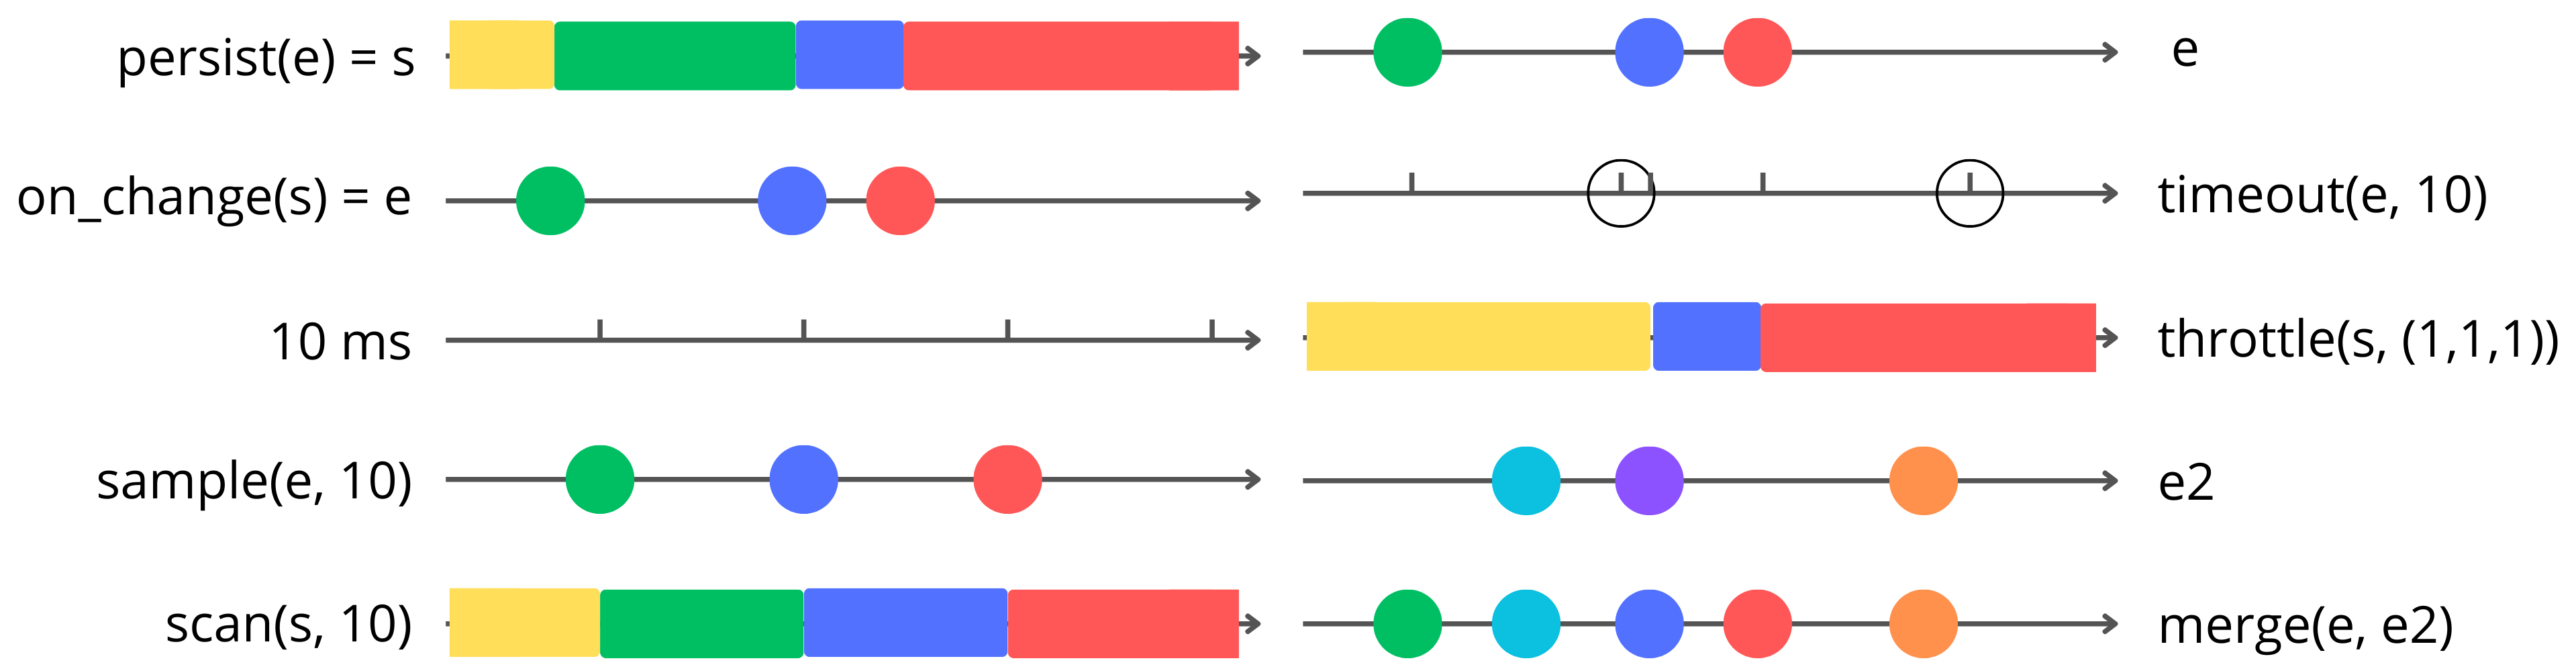
\includegraphics[width=\textwidth]{../images/greact.png}
    \caption[Chronograms of \GReact operators.]
    {Chronograms of \GReact operators (\texttt{10 ms} is used for \kft{sample} and \kft{scan}).}
    \label{fig:greact_operators}
\end{figure}

\subsection{Syntax of \GRSync}
\label{sec:grust:syntax:grsync}

This section presents \GRSync, a language for defining custom flow operators. Its syntax is shown in
EBNF notation in \Cref{fig:syntax:grsync}. \GRSync is highly inspired by \Lustre-like
languages~\cite{DBLP:conf/tase/ColacoPP17,DBLP:conf/hybrid/BourkeP13,DBLP:conf/emsoft/CohenGP12},
which bridge the gap between functional requirements and the implementation of critical systems.
These languages use \emph{clocks} to explicitly define when computations are performed. However,
correct usage of clocks often requires a deep understanding of the formal semantics of the language.
\GRSync omits explicit clocks and instead offers other constructs for filtering computations,
presented in the following paragraphs, that are tailored to needs in the automotive industry.

\begin{figure}[!ht]
    \centering
    \begin{bnf}(comment = {:is:})
        \FunItem ::= \funItem{\ID}{\many{(\ID \: \kft{:} \: \TY)}}{\TY}{\many{\Decl}} ;;
        \CompItem ::= \compItem{\ID}{\many{(\ID \: \kft{:} \: \STY)}}{\many{(\ID \: \kft{:} \: \STY)}}{\many{\Eq}} ;;
        \Eq ::= \Decl // \defEq{\many{\ID}}{\Expr} // \initEq{\ID}{\CST}
        | \matchX{\Expr}{\many{(\normBr{\gPat{\Pat}{\Expr}}{\setEq})}}
        | \whenEq{\initBr{\many{(\ID \: \kfm{=} \: \CST\kft{;})}}}{\many{(\normBr{\gPat{\EPat}{\Expr}}{\setEq})}} ;;
        \Decl ::= \declEq{\many{(\ID \: \kft{:} \: \STY)}}{\Expr} ;;
        \Expr ::= \CST // \ID // \lastExpr{\ID} // \emitExpr{\Expr} // \opExpr{\many{\Expr}} // \appExpr{\ID}{\many{\Expr}}
        | \matchX{\Expr}{\many{(\normBr{\gPat{\Pat}{\Expr}}{\Expr})}} ;;
        \Pat ::= \CST // \ID // \kft{\_} // \tuple{\Pat} ;;
        \EPat ::= \ID \kfm{=} \opt{\ID} // \Expr // \tuple{\EPat} ;;
        \STY ::= \TY // \opt{\TY} ;;
    \end{bnf}
    \caption[EBNF grammar of \GRSync.]%
    {EBNF grammar of \GRSync.
        Terminal symbols are in purple.
        Repetitions of \texttt{X} are denoted \many{\texttt{X}}.
        Option of \texttt{X} is denoted \texttt{X}?.
        \ID are identifiers composed of ASCII characters.
        \CST are constants.
        \OP represents $n$-ary operators (\eg addition).}
    \label{fig:syntax:grsync}
\end{figure}

User-defined flow operators are reusable building blocks, modeled as \emph{components} (\CompItem)
if they use a finite number of internal buffers, or as \emph{functions} (\FunItem) if they are
memory-free.

The signature of a component declares its name, and the sampling types and names of its input and
output flows.
%
The sampling type of a flow represents the type of the value present in that flow at any time.
For a signal \ID defined as \typed{\signalKind}{\ID}{\TY}, the sampling type is \TY as its value is
always present; for an event \ID defined as \typed{\eventKind}{\ID}{\TY}, the sampling type is the
option \opt{\TY} it might not have a value.
%
The body of a component is a set of mutually recursive equations (\setEq), stating the values
at every instant for the output flow based on the inputs. Ensuring that the output can be computed
at every time step is checked at compile-time, through an analysis called \emph{causality analysis}.
This is further explained in \Cref{sec:grust:implem:design_principles}.

The declaration of a function (\FunItem) is similar to that in traditional programming languages:
its signature declares a name, input flow names and types, and an output type. Its body contains an
ordered list of intermediary computations (\many{\Decl}) required to compute and return the output
(\kft{return} \Expr;). Functions operate on signal sampling types, as event handling typically
requires memory, which is reserved for components.

\GRSync offers the five kinds of equations that follow.
\begin{description}
    \item[Declaration] (\declEq{\many{(\ID:\STY)}}{\Expr}) defines local identifiers \many{\ID}.
    \item[Instantiation] (\defEq{\many{\ID}}{\Expr}) provides a definition for the outputs \many{\ID}.
    \item[Initialization] (\initEq{\ID}{\CST}) initializes a local signal \ID.
    \item[Match equation] (\matchX{\Expr}{\dots}) selects, for each instant, the first branch
          whose pattern (\Pat) matches the given expression and whose optional guard holds.
          Patterns can be constants, identifiers, wildcards, or tuples. Match equations must
          be exhaustive, ensuring a branch is always selected, and define the same identifiers.
    \item[When equation] (\whenEq{\initBr{\dots}}{\dots}) selects the first branch whose eventful
          pattern (\EPat) is satisfied and whose optional guard holds. An eventful pattern
          can be an event detection (\opt{\ID}), a rising edge detection (\Expr), or a
          conjunction of patterns. The activated branch performs punctual updates of signals
          and emissions of events. Signals not updated in a branch retain their previous
          values, which motivates their initialization in the \kft{init} branch.
\end{description}
Only declarations are used for intermediary computations in a function body.

Expressions are composed of constants (\CST), identifiers (\ID), $n$-ary operations
(\opExpr{\many{\Expr}}), component or function calls (\appExpr{\ID}{\many{\Expr}}), match
expressions (\matchX{\Expr}{\dots}), signal memories (\lastExpr{\ID}), and event emissions
(\emitExpr{\Expr}).

\subsection{Syntax of \GReusot}
\label{sec:grust:syntax:greusot}

\GRust enables formal verification by integrating with the \Creusot deductive verifier. This is
achieved through \GReusot, a language extension that allows developers to embed formal contracts
into \GRSync function and component declarations. The EBNF grammar governing these specifications is
detailed in \Cref{fig:syntax:greusot}.

\begin{figure}[!ht]
    \centering
    \begin{bnf}(comment = {:is:})
        \FunItem ::= \funItem[\Spec]{\ID}{\many{(\ID \: \kft{:} \: \TY)}}{\TY}{\many{\Decl}} ;;
        \CompItem ::= \compItem[\Spec]{\ID}{\many{(\ID \: \kft{:} \: \STY)}}
        {\many{(\ID \: \kft{:} \: \STY)}}{\many{\Eq}} ;;
        \Spec ::= \many{\Clause} ;;
        \Clause ::= \reqClause{\Term} // \ensClause{\Term} ;;
        \Term ::= \CST // \ID // \lastExpr{\ID} // \opExpr{\many{\Term}} // \tuple{\Term}
        // \appExpr{\ID}{\many{\Term}} | \implTerm{\Term}{\Term}
        // \forallTerm{\ID}{\TY}{\Term} | \whenTerm{\EPat}{\Term} // \resTerm ;;
    \end{bnf}
    \caption[EBNF grammar of \GReusot specifications.]{EBNF grammar of \GReusot specifications in component and function declarations.
        Terminal symbols are in purple. Repetitions of \texttt{X} are denoted \many{\texttt{X}}.
        \ID are identifiers. \CST are constants. \OP represents $n$-ary operators.}
    \label{fig:syntax:greusot}
\end{figure}

A specification (\Spec) is composed of one or more clauses (\Clause) that define preconditions
(\kft{requires}) and postconditions (\kft{ensures}). A precondition states the assumptions that must
be met for the function or component to execute correctly, while a postcondition describes the
properties that are guaranteed to hold upon completion.

These properties are expressed using logical terms (\Term). A term can be a constant (\CST), an
identifier (\ID), a reference to a past value (\lastExpr{\ID}), an $n$-ary operation
(\opExpr{\many{\Term}}), or a tuple (\tuple{\Term}). It can also represent a function call
(\appExpr{\ID}{\many{\Term}}), an implication (\implTerm{\Term}{\Term}), a universal quantifier
(\forallTerm{\ID}{\TY}{\Term}), or a conditional assertion based on an event
(\whenTerm{\EPat}{\Term}). For functions, the special term \resTerm refers to the return value.

\subsection{Summary}
This section has detailed the syntax of the \GRust language, which is structured around three core
elements and a proof extension. The high-level \GRFRP kernel is used to model asynchronous services
and define their external interfaces. The \GReact library provides a standard set of built-in
operators for common reactive patterns, inspired by \ReactiveX~\cite{reactivex}. For custom
operations, the \GRSync kernel offers a synchronous, equation-based language for defining stateful
components and stateless functions, using constructs like \texttt{when} and \texttt{match} for
controlled execution. Finally, the \GReusot extension integrates formal specification directly into
\GRSync, allowing developers to write contracts and prove critical properties. Together, these
elements form a comprehensive language for modeling, implementing, and verifying reactive systems.


\section{Identifiers Usage}
\label{sec:grust:id_usage}

This section formally defines the rules governing the use of identifiers in \GRust. A precise and
unambiguous specification of identifier scoping is essential for any programming language, as it
dictates where an identifier can be used and what it refers to. For a language like \GRust, intended
for critical systems, these rules are part of the language definition, ensuring predictable and
verifiable behavior.

The formal system presented here serves as a blueprint for the static analysis performed by the
compiler. It provides a rigorous foundation for implementing the symbol table, which tracks all
identifiers and their associated information, such as scope and type. By adhering to these rules,
the compiler can detect a range of errors at compile-time, including the use of undefined
identifiers, the redeclaration of an identifier within the same scope, and more subtle violations
specific to the structure of \GRust. For example, the logic enforces that all branches of a
\kft{match} equation must define the same set of identifiers, guaranteeing accessible values for
every execution.

This formalization addresses the two distinct scoping models within \GRust: the sequential, lexical
scoping of \GRFRP services and functions, and the mutually recursive scoping of \GRSync components.
The following logic, expressed through a set of inference rules, details how identifiers are
declared, defined, and used correctly across all language constructs.

\begin{table}[!ht]
    \centering
    \begin{tabularx}{\textwidth}{|l|X|}\hline
        $\ID_s, \: \ID_f, \: \ID_c, \: \ID$                                             & Service, function,
        component, and variable identifiers respectively.                                                                        \\\hline
        $\IDs ::= \{\ID^*\}$                                                            & A set of identifiers.                  \\\hline
        \begin{minipage}{0.37\textwidth}
            $\scope ::= \importScope \: \vert \: \exportScope \:
                \vert \:\inputScope$ \\ $\vert \: \outputScope \: \vert
                \: \localScope \: \vert \: \memoryScope$
        \end{minipage}                         & The scope of an identifier, such as an import, export,
        input, output, local, or component memory.                                                                               \\\hline
        $\G[\ID_s]$, $\G[\ID_f]$, $\G[\ID_c]$                                           & The identifier context maps
        service, function, or component identifiers to their definitions.                                                        \\\hline
        $\G[\ID] = \scope$                                                              & The identifier context maps a variable
        identifier to its scope.                                                                                                 \\\hline
        \idUsage{\G}{elem}{\texttt{Elem}}                                               & Asserts the correct usage
        of identifiers in the \GRust construct \texttt{Elem} with respect to the context \G.
        \\\hline
        \exports{(\Prog \: \vert \: \Item)}{\IDs}                                       & \IDs is the set of
        identifiers exported by program \Prog or item \Item.                                                                     \\\hline
        \declares{(\FlowStmt \: \vert \: \Eq \: \vert \: \Pat \: \vert \: \EPat)}{\IDs} & \IDs is the set of
        identifiers declared by statement \FlowStmt, equation \Eq or patterns \Pat and \EPat.                                    \\\hline
        \inits{\Eq}{\IDs}                                                               & \IDs is the set of
        identifiers initialized by equation \Eq.                                                                                 \\\hline
        \defines{(\Prog \: \vert \: \Item \: \vert \: \FlowStmt
        \: \vert \: \Eq)}{\IDs}                                                         & \IDs is the set of
        identifiers defined by program \Prog, item \Item, statement \FlowStmt, or equation \Eq, including declared ones.         \\\hline
    \end{tabularx}
    \caption[Notations for the usage of identifiers in \GRust.]%
    {Notations for the logic of identifier usage in \GRust.}
    \label{tab:grust:id_usage:notations}
\end{table}

We first introduce the notations for this logic, summarized in \Cref{tab:grust:id_usage:notations}.
The core of our formal system is the judgment \idUsage{\G}{elem}{\texttt{Elem}}, which asserts that
a \GRust construct \texttt{Elem} uses identifiers correctly with respect to an identifier context
\G. The context \G acts as a symbol table, mapping identifiers to their \emph{scope}, such as
\importScope, \outputScope, or \localScope. It also maps service, function, and component
identifiers ($\ID_s, \ID_f, \ID_c$) to their definitions.

To support this central judgment, we define several helper judgments that extract sets of
identifiers (\IDs) from various constructs:
\begin{itemize}
    \item \exports{\Prog \: \vert \: \Item}{\IDs} retrieves the set of identifiers that a program or
          item exports to the external environment.
    \item \declares{(\FlowStmt \: \vert \: \Eq \: \vert \: \Pat \: \vert \: \EPat)}{\IDs} retrieves
          the set of identifiers newly declared within a statement, an equation, or pattern.
    \item \inits{\Eq}{\IDs} retrieves the set of memory identifiers initialized in an equation.
    \item \defines{(\Prog \: \vert \: \Item \: \vert \: \FlowStmt \: \vert \: \Eq)}{\IDs} retrieves
          the set of identifiers that are given a definition. This includes both newly declared
          identifiers and existing ones (\eg component outputs).
\end{itemize}
The following paragraphs detail the rules for these judgments, explaining the logic of identifier
usage for each part of the \GRust language.

\subsection{\GRust Programs}
\label{sec:grust:id_usage:prog}

A \GRust program is well-formed if all its items are well-formed. The rule
\nameref{rule:grust:id_usage:program} formalizes this by checking each item individually. Crucially,
it also enforces a key property of a complete program: the set of identifiers it \emph{exports} must
be identical to the set it \emph{defines}. This ensures that every declared export has a
corresponding definition within a service, and that there are no definitions for non-exported flows
at the top level.

\begin{center}
    \begin{minipage}{0.9\textwidth}
        \centering
        \begin{mathpar}
            %% Program
            \inferID
            {
                \left(\itemIdUsage{\Item}\right)^* \\
                \exports{\Item^*}{\IDs} \\
                \defines{\Item^*}{\IDs}
            }
            { \progIdUsage{\Item^*} }
            {Prog}
            \label{rule:grust:id_usage:program}
        \end{mathpar}
    \end{minipage}
\end{center}

The good usage of an identifier in an item \Item with respect to the identifier context \G is
denoted by \itemIdUsage{\Item}. For interfaces, rules
\nameref{rule:grust:id_usage:interface:import} and
\nameref{rule:grust:id_usage:interface:export} ensure that imported and exported identifiers are
present in the context with the correct scope (\importScope for imports, and \exportScope for
exports).

\begin{center}
    \begin{minipage}{0.9\textwidth}
        \centering
        \begin{mathpar}
            %% Interface
            % Import
            \inferID
            { \G[\ID] = \importScope }
            { \itemIdUsage{\importX{\typed{\FlowKind}{\ID}{\TY}}} }
            {Import}
            \label{rule:grust:id_usage:interface:import}

            % Export
            \inferID
            { \G[\ID] = \exportScope }
            { \itemIdUsage{\exportX{\typed{\FlowKind}{\ID}{\TY}}} }
            {Export}
            \label{rule:grust:id_usage:interface:export}
        \end{mathpar}
    \end{minipage}
\end{center}

Rule \nameref{rule:grust:id_usage:service} states that for a service to be correct, its definition
must be in the context and its body must adhere to the identifier usage rules.

\begin{center}
    \begin{minipage}{0.9\textwidth}
        \centering
        \begin{mathpar}
            %% Service
            \inferID
            {
                \G[\ID_s] = \servItem{\ID_s}{\interval{\INT}{\INT}}{\many{\FlowStmt}} \\\\
                \stmtIdUsage{\G}{\many{\FlowStmt}}
            }
            { \itemIdUsage{\servItem{\ID_s}{\interval{\INT}{\INT}}{\many{\FlowStmt}}} }
            {Serv}
            \label{rule:grust:id_usage:service}
        \end{mathpar}
    \end{minipage}
\end{center}

For functions and components, the logic is similar. The rules ensure the item definition exists in
the context and that the body is well-formed. For a function, applying rule
\nameref{rule:grust:id_usage:fun}, the context is extended with its inputs before checking the body.
For a component, applying rule \nameref{rule:grust:id_usage:comp}, the context is extended with both
inputs and outputs to support the mutually recursive nature of its body.

\begin{center}
    \begin{minipage}{0.9\textwidth}
        \centering
        \begin{mathpar}
            %% Function
            \inferID
            {
                \G[\ID_f] = \funItem{\ID_f}{\many{(\ID_i \: \kft{:} \: \TY_i)}}{\TY_o}{\many{\Decl}} \\\\
                \G' = \G \ctxconcat [(\inputScope / \ID_i)^*] \\
                \declIdUsage{\G'}{\many{\Decl} \: \returnStmt{\Expr}}
            }
            { \itemIdUsage{\funItem{\ID_f}{\many{(\ID_i \: \kft{:} \: \TY_i)}}{\TY_o}{\many{\Decl}}} }
            {Fun}
            \label{rule:grust:id_usage:fun}
        \end{mathpar}
    \end{minipage}
\end{center}


\begin{center}
    \begin{minipage}{0.9\textwidth}
        \centering
        \begin{mathpar}
            %% Component
            \inferID
            {
                \G[\ID_c] = \compItem{\ID_c}{\many{(\ID_i \: \kft{:} \: \STY_i)}}{\many{(\ID_o \: \kft{:} \: \STY_o)}}{\many{\Eq}} \\\\
                \G' = \G \ctxconcat [(\inputScope / \ID_i)^*] \ctxconcat [(\outputScope / \ID_o)^*] \\\\
                \eqIdUsage{\G'}{\setEq} \\
                \defines{\setEq}{\IDs} \\
                \left(\ID_o \in \IDs\right)^*
            }
            { \itemIdUsage{\compItem{\ID_c}{\many{(\ID_i \: \kft{:} \: \STY_i)}}{\many{(\ID_o \: \kft{:} \: \STY_o)}}{\many{\Eq}}} }
            {Comp}
            \label{rule:grust:id_usage:comp}
        \end{mathpar}
    \end{minipage}
\end{center}

\paragraph{Exported identifiers}
\label{sec:grust:id_usage:prog:exported}

The judgment \exports{\Prog}{\IDs} computes the set of identifiers a program makes available
externally. As shown in rule \nameref{rule:grust:id_usage:prog:exported:program}, this is the union
of identifiers from all \kft{export} items. The use of the \emph{disjoint union} operator
($\bigsqcup$) enforces that each exported identifier must have a unique name across the entire
program, preventing ambiguity at the system level. The subsequent rules show that only \kft{export}
items contribute to this set.

\begin{center}
    \begin{minipage}{0.9\textwidth}
        \centering
        \begin{mathpar}
            %% Program
            \inferEXP
            { \left(\exports{\Item}{\IDs}\right)^* }
            { \exports{\Item^*}{\bigsqcup \IDs^*} }
            {Prog}
            \label{rule:grust:id_usage:prog:exported:program}
        \end{mathpar}
    \end{minipage}

    \begin{minipage}{0.99\textwidth}
        \centering
        \begin{mathpar}
            %% Interface
            % Import
            \inferEXP
            { }
            { \exports{\importX{\typed{\FlowKind}{\ID}{\TY}}}{\emptyset} }
            {Import}
            \label{rule:grust:id_usage:prog:exported:interface:import}

            % Export
            \inferEXP
            { }
            { \exports{\exportX{\typed{\FlowKind}{\ID}{\TY}}}{\{\ID\}} }
            {Export}
            \label{rule:grust:id_usage:prog:exported:interface:export}

            %% Service
            \inferEXP
            { }
            { \exports{\servItem{\ID_s}{\interval{\INT}{\INT}}{\many{\FlowStmt}}}{\emptyset} }
            {Serv}
            \label{rule:grust:id_usage:prog:exported:service}

            %% Function
            \inferEXP
            { }
            { \exports{\funItem{\ID_f}{\many{(\ID_i \: \kft{:} \: \TY_i)}}{\TY_o}{\many{\Decl}}}{\emptyset} }
            {Fun}
            \label{rule:grust:id_usage:prog:exported:fun}

            %% Component
            \inferEXP
            { }
            { \exports{\compItem{\ID_c}{\many{(\ID_i \: \kft{:} \: \STY_i)}}{\many{(\ID_o \: \kft{:} \: \STY_o)}}{\many{\Eq}}}{\emptyset} }
            {Comp}
            \label{rule:grust:id_usage:prog:exported:comp}
        \end{mathpar}
    \end{minipage}
\end{center}

\paragraph{Defined identifiers}
\label{sec:grust:id_usage:prog:defined}

The judgment \defines{\Prog}{\IDs} computes the set of identifiers defined within the services of a
program. Rule \nameref{rule:grust:id_usage:prog:defined:program} aggregates these identifiers from
all items, again using a disjoint union ($\bigsqcup$) to ensure that each defined identifier is
unique. As specified by the rules below, only instantiation statements (for exported flows) inside a
service contribute to this set.

\begin{center}
    \begin{minipage}{0.9\textwidth}
        \centering
        \begin{mathpar}
            \inferDEF
            { \left(\defines{\Item}{\IDs}\right)^* }
            { \defines{\Item^*}{\bigsqcup \IDs^*} }
            {Prog}
            \label{rule:grust:id_usage:prog:defined:program}
        \end{mathpar}
    \end{minipage}

    \begin{minipage}{0.9\textwidth}
        \centering
        \begin{mathpar}
            %% Interface
            % Import
            \inferDEF
            { }
            { \defines{\importX{\typed{\FlowKind}{\ID}{\TY}}}{\emptyset} }
            {Import}
            \label{rule:grust:id_usage:prog:defined:interface:import}

            % Export
            \inferDEF
            { }
            { \defines{\exportX{\typed{\FlowKind}{\ID}{\TY}}}{\emptyset} }
            {Export}
            \label{rule:grust:id_usage:prog:defined:interface:export}
        \end{mathpar}
    \end{minipage}

    \begin{minipage}{0.9\textwidth}
        \centering
        \begin{mathpar}
            %% Service
            \inferDEF
            {
                \declares{\block{\many{\FlowStmt}}}{\IDs_{\texttt{let}}} \\
                \defines{\block{\many{\FlowStmt}}}{\IDs_{\texttt{let}} \sqcup \IDs_{\texttt{export}}}
            }
            { \defines{\servItem{\ID_s}{\interval{\INT}{\INT}}{\many{\FlowStmt}}}{\IDs_{\texttt{export}}} }
            {Serv}
            \label{rule:grust:id_usage:prog:defined:service}

        \end{mathpar}
    \end{minipage}

    \begin{minipage}{0.9\textwidth}
        \centering
        \begin{mathpar}
            %% Function
            \inferDEF
            { }
            { \defines{\funItem{\ID_f}{\many{(\ID_i \: \kft{:} \: \TY_i)}}{\TY_o}{\many{\Decl}}}{\emptyset} }
            {Fun}
            \label{rule:grust:id_usage:prog:defined:fun}

        \end{mathpar}
    \end{minipage}

    \begin{minipage}{0.9\textwidth}
        \centering
        \begin{mathpar}
            %% Component
            \inferDEF
            { }
            { \defines{\compItem{\ID_c}{\many{(\ID_i \: \kft{:} \: \STY_i)}}{\many{(\ID_o \: \kft{:} \: \STY_o)}}{\many{\Eq}}}{\emptyset} }
            {Comp}
            \label{rule:grust:id_usage:prog:defined:comp}
        \end{mathpar}
    \end{minipage}
\end{center}

\subsection{Bodies of \GRFRP Services}
\label{sec:grust:id_usage:grfrp}

This part describes the correct usage of identifiers in services and all constructs of \GRFRP.

\subsubsection{Flow Statements}
\label{sec:grust:id_usage:grfrp:flow_stmt}

Flow statements in \GRFRP services follow a sequential, lexical scoping discipline. Identifiers are
introduced and are only visible to the statements that follow them in the same block. This is
captured by the judgment \stmtIdUsage{\G}{\FlowStmt^*}, which threads the identifier context \G
through the list of statements.

An empty block of statements is trivially well-formed, as stated by rule
\nameref{rule:grust:id_usage:grfrp:flow_stmt:skip}.
A \kft{let} statement introduces new local identifiers: rule
\nameref{rule:grust:id_usage:grfrp:flow_stmt:let} checks the right-hand side of the declaration
before extending the context \G with these new identifiers for the subsequent statements. This
ensures the new identifiers are available in the rest of the scope but not in their own definition.
In contrast, a definition statement assigns a flow to an existing, exported identifier: rule
\nameref{rule:grust:id_usage:grfrp:flow_stmt:def} verifies that the identifier has already been
declared with \exportScope and then checks the remaining statements with the original context.

\begin{center}
    \begin{minipage}{0.9\textwidth}
        \centering
        \begin{mathpar}
            %% Flow Statement
            % Skip
            \inferIDFlowStmt
            { }
            { \stmtIdUsage{\G}{} }
            {Skip}
            \label{rule:grust:id_usage:grfrp:flow_stmt:skip}

            % Let
            \inferIDFlowStmt
            {
                \flowIdUsage{\G}{\FlowOp} \\
                \G' = \G \ctxconcat [(\localScope / \ID)^*] \\
                \stmtIdUsage{\G'}{\FlowStmt^*}
            }
            { \stmtIdUsage{\G}{\letStmt{\many{(\typed{\FlowKind}{\ID}{\TY})}}{\FlowOp} \: \FlowStmt^*} }
            {Let}
            \label{rule:grust:id_usage:grfrp:flow_stmt:let}

            % Definition
            \inferIDFlowStmt
            {
                \left(\G[\ID] = \exportScope\right)^* \\
                \flowIdUsage{\G}{\FlowOp} \\
                \stmtIdUsage{\G}{\FlowStmt^*}
            }
            { \stmtIdUsage{\G}{\defStmt{\many{\ID}}{\FlowOp} \: \FlowStmt^*} }
            {Def}
            \label{rule:grust:id_usage:grfrp:flow_stmt:def}
        \end{mathpar}
    \end{minipage}
\end{center}

\paragraph{Declared identifiers}
\label{sec:grust:id_usage:grfrp:flow_stmt:declared}

The set of declared identifiers in a flow statement is computed by the judgment
\declares{\FlowStmt}{\IDs}. Rules \nameref{sec:grust:id_usage:grfrp:flow_stmt:declared:let}
and \nameref{sec:grust:id_usage:grfrp:flow_stmt:declared:def} ensure that only \kft{let}
statements contribute to the set of declared identifiers at program-level.

\begin{center}
    \begin{minipage}{0.9\textwidth}
        \centering
        \begin{mathpar}
            \inferDECLFlowStmt
            { }
            { \declares{\letStmt{\many{(\ldots)}}{\ldots} \: \FlowStmt^*}{\{\many{\ID}\}} }
            {Let}
            \label{sec:grust:id_usage:grfrp:flow_stmt:declared:let}

            \inferDECLFlowStmt
            { }
            { \declares{\defStmt{\many{\ID}}{\ldots} \: \FlowStmt^*}{\emptyset} }
            {Def}
            \label{sec:grust:id_usage:grfrp:flow_stmt:declared:def}
        \end{mathpar}
    \end{minipage}
\end{center}

\paragraph{Defined identifiers}
\label{sec:grust:id_usage:grfrp:flow_stmt:defined}

The set of defined identifiers in a flow statement is computed by the judgment
\defines{\FlowStmt}{\IDs}. Rules \nameref{sec:grust:id_usage:grfrp:flow_stmt:defined:let}
and \nameref{sec:grust:id_usage:grfrp:flow_stmt:defined:def} specify that all statements contribute
to the set of defined identifiers for the program-level check.

\begin{center}
    \begin{minipage}{0.9\textwidth}
        \centering
        \begin{mathpar}
            \inferDEFFlowStmt
            { }
            { \defines{\letStmt{\many{(\typed{\FlowKind}{\ID}{\TY})}}{\FlowOp} \: \FlowStmt^*}{\{\many{\ID}\}} }
            {Let}
            \label{sec:grust:id_usage:grfrp:flow_stmt:defined:let}

            \inferDEFFlowStmt
            { }
            { \defines{\defStmt{\many{\ID}}{\FlowOp} \: \FlowStmt^*}{\{\many{\ID}\}} }
            {Def}
            \label{sec:grust:id_usage:grfrp:flow_stmt:defined:def}
        \end{mathpar}
    \end{minipage}
\end{center}

\subsubsection{Flow Operations}
\label{sec:grust:id_usage:grfrp:flow_op}

The judgment \flowIdUsage{\G}{\FlowOp} checks that a flow operation uses identifiers
correctly. The rules ensure that any used identifier, function, or component is present in
the context \G and that all sub-expressions are themselves well-formed.

\begin{center}
    \begin{minipage}{0.99\textwidth}
        \centering
        \begin{mathpar}
            %% Flow Operation
            % Identifier
            \inferIDFlow
            { \G[\ID] = \scope }
            { \flowIdUsage{\G}{\ID} }
            {ID}
            \label{rule:grust:id_usage:grfrp:flow_op:ident}

            %% Application
            % Function
            \inferIDFlow
            {
                \G[\ID_f] = \funItem{\ID_f}{\many{(\ID_i \: \kft{:} \: \TY_i)}}{\TY_o}{\many{\Decl}} \\\\
                \left(\flowIdUsage{\G}{\FlowOp}\right)^*
            }
            { \flowIdUsage{\G}{\compApp{\ID_f}{\many{\FlowOp}}} }
            {AppF}
            \label{rule:grust:id_usage:grfrp:flow_op:funapp}

            % Component
            \inferIDFlow
            {
                \G[\ID_c] = \compItem{\ID_c}{\many{(\ID_i \: \kft{:} \: \STY_i)}}{\many{(\ID_o \: \kft{:} \: \STY_o)}}{\many{\Eq}} \\\\
                \left(\flowIdUsage{\G}{\FlowOp}\right)^*
            }
            { \flowIdUsage{\G}{\compApp{\ID_c}{\many{\FlowOp}}} }
            {AppC}
            \label{rule:grust:id_usage:grfrp:flow_op:compapp}
        \end{mathpar}
    \end{minipage}
\end{center}

\GReact operations are checked by ensuring their input flow operations are well-formed.

\begin{center}
    \begin{minipage}{0.9\textwidth}
        \centering
        \begin{mathpar}
            %% GReact
            % OnChange
            \inferIDFlow
            { \flowIdUsage{\G}{\FlowOp} }
            { \flowIdUsage{\G}{\onchangeExpr{\FlowOp}} }
            {OChg}
            \label{rule:grust:id_usage:grfrp:flow_op:onchange}

            % Persist
            \inferIDFlow
            { \flowIdUsage{\G}{\FlowOp} }
            { \flowIdUsage{\G}{\persistExpr{\FlowOp}} }
            {Prst}
            \label{rule:grust:id_usage:grfrp:flow_op:persist}

            % Scan
            \inferIDFlow
            { \flowIdUsage{\G}{\FlowOp} }
            { \flowIdUsage{\G}{\scanExpr{\FlowOp}{\INT}} }
            {Scan}
            \label{rule:grust:id_usage:grfrp:flow_op:scan}

            % Sample
            \inferIDFlow
            { \flowIdUsage{\G}{\FlowOp} }
            { \flowIdUsage{\G}{\scanExpr{\FlowOp}{\INT}} }
            {Samp}
            \label{rule:grust:id_usage:grfrp:flow_op:sample}

            % Timeout
            \inferIDFlow
            { \flowIdUsage{\G}{\FlowOp} }
            { \flowIdUsage{\G}{\timeoutExpr{\FlowOp}{\INT}} }
            {TOut}
            \label{rule:grust:id_usage:grfrp:flow_op:timeout}

            % Merge
            \inferIDFlow
            {
                \flowIdUsage{\G}{\FlowOp_1} \\
                \flowIdUsage{\G}{\FlowOp_2}
            }
            { \flowIdUsage{\G}{\mergeExpr{\FlowOp_1}{\FlowOp_2}} }
            {Mrg}
            \label{rule:grust:id_usage:grfrp:flow_op:merge}

            % Throttle
            \inferIDFlow
            { \flowIdUsage{\G}{\FlowOp} }
            { \flowIdUsage{\G}{\throttleExpr{\FlowOp}{\DELTA}} }
            {Thrt}
            \label{rule:grust:id_usage:grfrp:flow_op:throttle}

            % Time
            \inferIDFlow
            { }
            { \flowIdUsage{\G}{\timeExpr} }
            {Time}
            \label{rule:grust:id_usage:grfrp:flow_op:time}
        \end{mathpar}
    \end{minipage}
\end{center}

\subsection{Bodies of \GRSync Functions and Components}
\label{sec:grust:id_usage:grsync}

This part describes the correct usage of identifiers in functions and components.

\subsubsection{Function Declarations}
\label{sec:grust:id_usage:grsync:fun_decl}

Declarations in functions, like statements in services, are ordered and lexically scoped. The
judgment \declIdUsage{\G}{\many{\Decl} \: \returnStmt{\Expr}} checks a block of declarations
followed by a return statement. Rule \nameref{rule:grust:id_usage:grsync:fun_decl:decl} extends the
context with newly declared local identifiers before checking the subsequent declarations and the
final return statement with \nameref{rule:grust:id_usage:grsync:fun_decl:return}.

\begin{center}
    \begin{minipage}{0.9\textwidth}
        \centering
        \begin{mathpar}
            %% Return
            \inferIDDecl
            { \exprIdUsage{\G}{\Expr} }
            { \declIdUsage{\G}{\returnStmt{\Expr}} }
            {Ret}
            \label{rule:grust:id_usage:grsync:fun_decl:return}


            %% Declarations
            \inferIDDecl
            {
                \G' = \G \ctxconcat [(\localScope / \ID)^*] \\
                \declIdUsage{\G'}{\many{\Decl} \: \returnStmt{\Expr}}
            }
            { \declIdUsage{\G}{\declEq{\many{(\ID \: \kft{:} \: \STY)}}{\Expr} \: \many{\Decl} \: \returnStmt{\Expr}} }
            {Decl}
            \label{rule:grust:id_usage:grsync:fun_decl:decl}
        \end{mathpar}
    \end{minipage}
\end{center}

\subsubsection{Component Equations}
\label{sec:grust:id_usage:grsync:eq}

In contrast to the sequential nature of services and function, equations within \GRSync components
follow a mutually recursive scoping model. All identifiers declared locally or as state memories
within a component body are visible throughout that entire body, including in their own definitions.
This allows for defining interdependent dataflow equations without regard to textual order.

Rule \nameref{rule:grust:id_usage:grsync:eqs} formalizes this by first collecting all locally
declared identifiers ($\ID_l^*$) and memory identifiers ($\ID_m^*$) from the set of equations
\setEq. It then extends the context \G with these identifiers to create a new context \G', which is
subsequently used to check each individual equation in the set. The use of disjoint union in the
helper judgments ensures that each local and memory identifier is declared at most once.

\begin{center}
    \begin{minipage}{0.9\textwidth}
        \centering
        \begin{mathpar}
            %% Set of equations
            \inferIDEq
            {
                \declares{\setEq}{\{\ID_l^*\}} \\
                \inits{\setEq}{\{\ID_m^*\}} \\
                \G' = \G \ctxconcat [(\localScope / \ID_l)^*] \ctxconcat [(\memoryScope / \ID_m)^*] \\
                \left(\eqIdUsage{\G'}{\Eq}\right)^*
            }
            { \eqIdUsage{\G}{\setEq} }
            {Blck}
            \label{rule:grust:id_usage:grsync:eqs}
        \end{mathpar}
    \end{minipage}
\end{center}

Individual declaration, definition, and initialization equations are checked to ensure they assign
to identifiers of the correct scope (\localScope, \outputScope, and \memoryScope, respectively), as
described by the rules \nameref{rule:grust:id_usage:grsync:eq:decl},
\nameref{rule:grust:id_usage:grsync:eq:def}, and \nameref{rule:grust:id_usage:grsync:eq:init}.

\begin{center}
    \begin{minipage}{0.9\textwidth}
        \centering
        \begin{mathpar}
            %% Declarations
            \inferIDEq
            {
                \left(\G[\ID] = \localScope\right)^* \\
                \exprIdUsage{\G}{\Expr}
            }
            { \eqIdUsage{\G}{\declEq{\many{(\ID \: \kft{:} \: \STY)}}{\Expr}} }
            {Decl}
            \label{rule:grust:id_usage:grsync:eq:decl}

            %% Definition
            \inferIDEq
            {
                \left(\G[\ID] = \outputScope\right)^* \\
                \exprIdUsage{\G}{\Expr}
            }
            { \eqIdUsage{\G}{\defEq{\many{\ID}}{\Expr}} }
            {Def}
            \label{rule:grust:id_usage:grsync:eq:def}

            %% Initialization
            \inferIDEq
            { \G[\lastExpr{\ID}] = \memoryScope }
            { \eqIdUsage{\G}{\initEq{\ID}{\CST}} }
            {Init}
            \label{rule:grust:id_usage:grsync:eq:init}
        \end{mathpar}
    \end{minipage}
\end{center}

The rule for a \kft{match} equation formalizes how identifiers are scoped within a conditional block
that branches on the value of an expression. First, it asserts that the expression being matched
must be valid in the surrounding context. Then, for each branch of the \kft{match}, the rule
specifies that a new, temporary scope is created. This branch-specific scope contains all the
identifiers from the outer scope, plus any new local identifiers that are bound by that branch's
pattern. The guard condition and the equations within the branch body are then validated using this
temporary scope. This ensures that the logic inside a branch can safely use the variables
deconstructed from the pattern, while also guaranteeing that these variables are properly isolated
and do not leak into sibling branches or the surrounding scope.

\begin{center}
    \begin{minipage}{0.9\textwidth}
        \centering
        \begin{mathpar}
            %% Match
            \inferIDEq
            {
                \exprIdUsage{\G}{\Expr} \\
                \left(\declares{\Pat_k}{\{\ID_k^*\}}\right)^* \\
                \left(\G_k = \G \ctxconcat [(\localScope / \ID_k)^*] \right)^* \\
                \left(\exprIdUsage{\G_k}{\Expr_k}\right)^* \\
                \left(\eqIdUsage{\G_k}{\setEq[k]}\right)^*
            }
            { \eqIdUsage{\G}{\matchX{\Expr}{\many{(\normBr{\gPat{\Pat_k}{\Expr_k}}{\setEq[k]})}}} }
            {Mtch}
            \label{rule:grust:id_usage:grsync:eq:match}
        \end{mathpar}
    \end{minipage}
\end{center}

The rule for a \kft{when} equation defines the scoping for event-driven logic, where a block of
equations is executed in response to an event. The logic proceeds as follows: for each branch, it
first verifies that the event pattern is valid, meaning it refers to a known event. It then
identifies any new local variables that are bound by the pattern, which correspond to the data
payload carried by the event. Similar to a \kft{match} equation, a temporary, branch-specific scope
is created that includes these new payload variables. Finally, the guard condition and the body of
equations for that branch are validated within this temporary scope. This formalizes a safe
mechanism for handling event data, ensuring that the payload of an event is only accessible to the
code block designated to process it.

\begin{center}
    \begin{minipage}{0.99\textwidth}
        \centering
        \begin{mathpar}
            %% When
            \inferIDEq
            {
                \left(\epatIdUsage{\G}{\EPat_k}\right)^* \\
                \left(\declares{\EPat_k}{\{\ID_k^*\}}\right)^* \\\\
                \left(\G_k = \G \ctxconcat [(\localScope / \ID_k)^*] \right)^* \\
                \left(\exprIdUsage{\G_k}{\Expr_k}\right)^* \\
                \left(\eqIdUsage{\G_k}{\setEq[k]}\right)^*
            }
            { \eqIdUsage{\G}{\whenEq{\initBr{\many{(\ID \: \kfm{=} \: \CST\kft{;})}}}{\many{(\normBr{\gPat{\EPat_k}{\Expr_k}}{\setEq[k]})}}} }
            {When}
            \label{rule:grust:id_usage:grsync:eq:when}
        \end{mathpar}
    \end{minipage}
\end{center}

\paragraph{Declared identifiers}
\label{sec:grust:id_usage:grsync:eq:declared}

The judgment \declares{\Eq}{\IDs} collects newly introduced identifiers. The use of disjoint union
($\bigsqcup$) in rule \nameref{rule:grust:id_usage:grsync:eq:declared:eqs} ensures that an
identifier is declared only once in a block of equations.

\begin{center}
    \begin{minipage}{0.9\textwidth}
        \centering
        \begin{mathpar}
            %% Set of equations
            \inferDECLEq
            { \left(\declares{\Eq}{\IDs}\right)^* }
            { \declares{\setEq}{\bigsqcup \IDs^*} }
            {Blck}
            \label{rule:grust:id_usage:grsync:eq:declared:eqs}

            %% Declarations
            \inferDECLEq
            { }
            { \declares{\declEq{\many{(\ID \: \kft{:} \: \STY)}}{\Expr}}{\{\ID^*\}} }
            {Decl}
            \label{rule:grust:id_usage:grsync:eq:declared:decl}

            %% Definition
            \inferDECLEq
            { }
            { \declares{\defEq{\many{\ID}}{\Expr}}{\emptyset} }
            {Def}
            \label{rule:grust:id_usage:grsync:eq:declared:def}

            %% Initialization
            \inferDECLEq
            { }
            { \declares{\initEq{\ID}{\CST}}{\emptyset} }
            {Init}
            \label{rule:grust:id_usage:grsync:eq:declared:init}
        \end{mathpar}
    \end{minipage}
\end{center}

The scoping rules for \kft{match} and \kft{when} equations reflect a fundamental distinction in
their purpose.

A \kft{match} equation defines flows based on pattern matching. As defined by rule
\nameref{rule:grust:id_usage:grsync:eq:declared:match}, all branches must declare an identical set
of identifiers. This ensures that a \kft{match} equation is sound: it always computes a complete and
consistent set of outputs. Regardless of which branch is executed, dependent computations can rely
on the same set of identifiers being available, which prevents the possibility of undefined
behavior.

In contrast, a \kft{when} equation is designed for event-driven \emph{updates}. Rule
\nameref{rule:grust:id_usage:grsync:eq:declared:when} allows each branch to declare a different set
of identifiers, enabling partial state changes. If a signal is not declared in a branch, its value
is not updated when that branch is active and retains its previous value. This persistence model
explains why signals in a \kft{when} construct must be initialized. Similarly, an event is emitted
only if it is declared in the active branch.

\begin{center}
    \begin{minipage}{0.95\textwidth}
        \centering
        \begin{mathpar}
            %% Match
            \inferDECLEq
            { \left(\declares{\setEq[k]}{\IDs}\right)^* }
            { \declares{\matchX{\Expr}{\many{(\normBr{\gPat{\Pat_k}{\Expr_k}}{\setEq[k]})}}}{\IDs} }
            {Mtch}
            \label{rule:grust:id_usage:grsync:eq:declared:match}

            %% When
            \inferDECLEq
            { \left(\declares{\setEq[k]}{\IDs}\right)^* }
            { \declares{
                    \whenEq{\initBr{\many{(\ID \: \kfm{=} \: \CST\kft{;})}}}
                    {\ldots}
                }{\bigcup \IDs^*} }
            {When}
            \label{rule:grust:id_usage:grsync:eq:declared:when}
        \end{mathpar}
    \end{minipage}
\end{center}

\paragraph{Initialized identifiers}
\label{sec:grust:id_usage:grsync:eq:initialized}

The judgment \inits{\Eq}{\IDs} collects the identifiers of signals that require memory. In \GRSync,
such stateful signals can only be initialized at the top level of a component or within a \kft{when}
equation, following rule \nameref{rule:grust:id_usage:grsync:eq:initialized:when}. The latter is
permitted because \kft{when} constructs are specifically designed for event-triggered state updates.
In contrast, \kft{match} equations describe control flow logic. Consequently, rule
\nameref{rule:grust:id_usage:grsync:eq:initialized:match} prohibits the initialization of new
memories within the branches of a \kft{match}.

\begin{center}
    \begin{minipage}{0.95\textwidth}
        \centering
        \begin{mathpar}
            %% Set of equations
            \inferINITEq
            { \left(\inits{\Eq}{\IDs}\right)^* }
            { \inits{\setEq}{\bigsqcup \IDs^*} }
            {Blck}
            \label{rule:grust:id_usage:grsync:eq:initialized:eqs}

            %% Declarations
            \inferINITEq
            { }
            { \inits{\declEq{\many{(\ID \: \kft{:} \: \STY)}}{\Expr}}{\emptyset} }
            {Decl}
            \label{rule:grust:id_usage:grsync:eq:initialized:decl}

            %% Definition
            \inferINITEq
            { }
            { \inits{\defEq{\many{\ID}}{\Expr}}{\emptyset} }
            {Def}
            \label{rule:grust:id_usage:grsync:eq:initialized:def}

            %% Initialization
            \inferINITEq
            { }
            { \inits{\initEq{\ID}{\CST}}{\{\lastExpr{\ID}\}} }
            {Init}
            \label{rule:grust:id_usage:grsync:eq:initialized:init}
        \end{mathpar}
    \end{minipage}

    \begin{minipage}{0.99\textwidth}
        \centering
        \begin{mathpar}
            %% Match
            \inferINITEq
            { \left(\inits{\setEq[k]}{\emptyset}\right)^* }
            { \inits{\matchX{\Expr}{\many{(\normBr{\gPat{\Pat_k}{\Expr_k}}{\setEq[k]})}}}{\emptyset} }
            {Mtch}
            \label{rule:grust:id_usage:grsync:eq:initialized:match}

            %% When
            \inferINITEq
            { \IDs = \{(\lastExpr{\ID})^*\} \\ \left(\inits{\setEq[k]}{\emptyset}\right)^* }
            { \inits{
                    \whenEq{\initBr{\many{(\ID \: \kfm{=} \: \CST\kft{;})}}}
                    {\many{(\normBr{\gPat{\EPat_k}{\Expr_k}}{\setEq[k]})}}
                }{\IDs} }
            {When}
            \label{rule:grust:id_usage:grsync:eq:initialized:when}
        \end{mathpar}
    \end{minipage}
\end{center}

\paragraph{Defined identifiers}
\label{sec:grust:id_usage:grsync:eq:defined}

The judgment \defines{\Eq}{\IDs} collects all identifiers assigned a value in an equation \Eq.

For a \kft{match} equation, rule \nameref{rule:grust:id_usage:grsync:eq:defined:match} requires the
set of defined identifiers to be identical across all branches. This aligns with the role of a
\kft{match}: it guarantees that a complete and consistent set of outputs is always produced,
regardless of which branch is executed.

In contrast, a \kft{when} equation enables selective updates. Rule
\nameref{rule:grust:id_usage:grsync:eq:defined:when} defines its set of identifiers as the union of
those in its branches. This mechanism allows a branch to specify only the flows it needs to change.
If a signal is not defined in the active branch, it retains its previous value, while an undefined
event is not emitted.

\begin{center}
    \begin{minipage}{0.95\textwidth}
        \centering
        \begin{mathpar}
            %% Set of equations
            \inferDEFEq
            { \left(\defines{\Eq}{\IDs}\right)^* }
            { \defines{\setEq}{\bigsqcup \IDs^*} }
            {Blck}
            \label{rule:grust:id_usage:grsync:eq:defined:eqs}

            %% Declarations
            \inferDEFEq
            { }
            { \defines{\declEq{\many{(\ID \: \kft{:} \: \STY)}}{\Expr}}{\{\ID^*\}} }
            {Decl}
            \label{rule:grust:id_usage:grsync:eq:defined:decl}

            %% Definition
            \inferDEFEq
            { }
            { \defines{\defEq{\many{\ID}}{\Expr}}{\{\ID^*\}} }
            {Def}
            \label{rule:grust:id_usage:grsync:eq:defined:def}

            %% Initialization
            \inferDEFEq
            { }
            { \defines{\initEq{\ID}{\CST}}{\emptyset} }
            {Init}
            \label{rule:grust:id_usage:grsync:eq:defined:init}
        \end{mathpar}
    \end{minipage}

    \begin{minipage}{0.95\textwidth}
        \centering
        \begin{mathpar}
            %% Match
            \inferDEFEq
            { \left(\defines{\setEq[k]}{\{\ID^*\}}\right)^* }
            { \defines{\matchX{\Expr}{\many{(\normBr{\gPat{\Pat_k}{\Expr_k}}{\setEq[k]})}}}{\{\ID^*\}} }
            {Mtch}
            \label{rule:grust:id_usage:grsync:eq:defined:match}

            %% When
            \inferDEFEq
            { \left(\defines{\setEq[k]}{\IDs}\right)^* }
            { \defines{
                    \mathfoot{\whenEq{\initBr{\many{(\ID \: \kfm{=} \: \CST\kft{;})}}}
                        {\many{(\normBr{\gPat{\EPat_k}{\Expr_k}}{\setEq[k]})}}}
                }{\bigcup \IDs^*} }
            {When}
            \label{rule:grust:id_usage:grsync:eq:defined:when}
        \end{mathpar}
    \end{minipage}
\end{center}

\subsubsection{Expressions}
\label{sec:grust:id_usage:grsync:expr}

The judgment \exprIdUsage{\G}{\Expr} verifies that all identifiers in an expression \Expr are used
correctly according to the context \G.

The simplest expressions involve constants, identifiers, and memory access. Rule
\nameref{rule:grust:id_usage:grsync:expr:const} states that a constant is always valid. Rule
\nameref{rule:grust:id_usage:grsync:expr:id} requires that an identifier \ID be present in the
context. Rule \nameref{rule:grust:id_usage:grsync:expr:last} allows accessing the previous value of
a signal with \lastExpr{\ID} only if the identifier has \memoryScope, ensuring it is a stateful
signal.

\begin{center}
    \begin{minipage}{0.9\textwidth}
        \centering
        \begin{mathpar}
            %% Constant
            \inferIDE
            {  }
            { \exprIdUsage{\G}{\CST} }
            {Cst}
            \label{rule:grust:id_usage:grsync:expr:const}

            %% Identifier
            \inferIDE
            { \G[\ID] = \scope }
            { \exprIdUsage{\G}{\ID} }
            {ID}
            \label{rule:grust:id_usage:grsync:expr:id}

            %% Last
            \inferIDE
            { \G[\lastExpr{\ID}] = \memoryScope }
            { \exprIdUsage{\G}{\lastExpr{\ID}} }
            {Last}
            \label{rule:grust:id_usage:grsync:expr:last}
        \end{mathpar}
    \end{minipage}
\end{center}

For composite expressions, validation is recursive. Rules
\nameref{rule:grust:id_usage:grsync:expr:emit} and \nameref{rule:grust:id_usage:grsync:expr:op}
state that an event emission or an $n$-ary operation is valid if all its sub-expressions are valid.

\begin{center}
    \begin{minipage}{0.9\textwidth}
        \centering
        \begin{mathpar}
            %% Emit
            \inferIDE
            { \exprIdUsage{\G}{\Expr} }
            { \exprIdUsage{\G}{\emitExpr{\Expr}} }
            {Emit}
            \label{rule:grust:id_usage:grsync:expr:emit}

            %% $n$-ary operation
            \inferIDE
            { \left(\exprIdUsage{\G}{\Expr}\right)^* }
            { \exprIdUsage{\G}{\opExpr{\many{\Expr}}} }
            {Op}
            \label{rule:grust:id_usage:grsync:expr:op}
        \end{mathpar}
    \end{minipage}
\end{center}

Function and component applications are handled by rules
\nameref{rule:grust:id_usage:grsync:expr:funapp} and
\nameref{rule:grust:id_usage:grsync:expr:compapp}. These rules require that the called function or
component is defined in the context and that all argument expressions are valid.

\begin{center}
    \begin{minipage}{0.99\textwidth}
        \centering
        \begin{mathpar}
            %% Application
            % Function
            \inferIDE
            {
                \G[\ID_f] = \funItem{\ID_f}{\many{(\ID_i \: \kft{:} \: \TY_i)}}{\TY_o}{\many{\Decl}} \\\\
                \left(\exprIdUsage{\G}{\Expr}\right)^*
            }
            { \exprIdUsage{\G}{\appExpr{\ID_f}{\many{\Expr}}} }
            {AppF}
            \label{rule:grust:id_usage:grsync:expr:funapp}

            % Component
            \inferIDE
            {
                \G[\ID_c] = \compItem{\ID_c}{\many{(\ID_i \: \kft{:} \: \STY_i)}}{\many{(\ID_o \: \kft{:} \: \STY_o)}}{\many{\Eq}} \\\\
                \left(\exprIdUsage{\G}{\Expr}\right)^*
            }
            { \exprIdUsage{\G}{\appExpr{\ID_c}{\many{\Expr}}} }
            {AppC}
            \label{rule:grust:id_usage:grsync:expr:compapp}
        \end{mathpar}
    \end{minipage}
\end{center}

For a \kft{match} expression, rule \nameref{rule:grust:id_usage:grsync:expr:match} imposes several
conditions. First, the matched expression \Expr must be valid in the current context \G. Then, for
each branch, the identifiers declared in the pattern $\Pat_k$ are added to the context, creating a
local context $\G_k$. Both the guard and the body expressions of that branch must be valid in this
extended local context.

\begin{center}
    \begin{minipage}{0.9\textwidth}
        \centering
        \begin{mathpar}
            %% Match
            \inferIDE
            {
                \exprIdUsage{\G}{\Expr} \\
                \left(\declares{\Pat_k}{\{\ID_k^*\}}\right)^* \\
                \left(\G_k = \G \ctxconcat [(\localScope / \ID_k)^*] \right) \\
                \left(\exprIdUsage{\G_k}{\Expr_k^g}\right)^* \\
                \left(\exprIdUsage{\G_k}{\Expr_k}\right)^*
            }
            { \exprIdUsage{\G}{\matchX{\Expr}{\many{(\normBr{\gPat{\Pat_k}{\Expr_k^g}}{\Expr_k})}}} }
            {Mtch}
            \label{rule:grust:id_usage:grsync:expr:match}
        \end{mathpar}
    \end{minipage}
\end{center}

\subsubsection{Patterns}
\label{sec:grust:id_usage:grsync:pat}

Patterns do not use identifiers from the context; instead, they declare new identifiers that are
local to the branch where they appear.

\paragraph{Declared identifiers}
\label{sec:grust:id_usage:grsync:pat:declared}

The judgment \declares{\Pat}{\IDs} collects the set of identifiers \IDs declared by a pattern
\Pat. The rules show that only identifier patterns contribute to this set. Constants, wildcards, and
other structural patterns do not declare any identifiers, while tuple patterns aggregate with a
disjoint union the identifiers from their sub-patterns.

\begin{center}
    \begin{minipage}{0.9\textwidth}
        \centering
        \begin{mathpar}
            %% Constant
            \inferDECLPat
            { }
            { \declares{\CST}{\emptyset} }
            {Cst}
            \label{rule:grust:id_usage:grsync:pat:declared:const}

            %% Identifier
            \inferDECLPat
            { }
            { \declares{\ID}{\{\ID\}} }
            {ID}
            \label{rule:grust:id_usage:grsync:pat:declared:id}

            %% Wildcard
            \inferDECLPat
            { }
            { \declares{\_}{\emptyset} }
            {Wild}
            \label{rule:grust:id_usage:grsync:pat:declared:wild}

            %% Tuple
            \inferDECLPat
            { \left(\declares{\Pat}{\IDs}\right)^* }
            { \declares{\tuple{\Pat}}{\bigsqcup \IDs^*} }
            {Tupl}
            \label{rule:grust:id_usage:grsync:pat:declared:tuple}
        \end{mathpar}
    \end{minipage}
\end{center}

\subsubsection{Event Patterns}
\label{sec:grust:id_usage:grsync:epat}

The judgment \epatIdUsage{\G}{\EPat} validates the use of identifiers within an event pattern \EPat.

Rule \nameref{rule:grust:id_usage:grsync:epat:event} handles event detection, ensuring the source
event $\ID_e$ is defined in the context. Rule \nameref{rule:grust:id_usage:grsync:epat:edge} handles
rising edges, requiring the underlying boolean expression \Expr to be valid. A tuple of event
patterns is valid if each constituent pattern is valid, as specified by rule
\nameref{rule:grust:id_usage:grsync:epat:tuple}.

\begin{center}
    \begin{minipage}{0.9\textwidth}
        \centering
        \begin{mathpar}
            %% Event detection
            \inferIDEPat
            { \G[\ID_e] = \scope }
            { \epatIdUsage{\G}{\ID \: \kfm{=} \: \opt{\ID_e}} }
            {Dtct}
            \label{rule:grust:id_usage:grsync:epat:event}

            %% Rising edge
            \inferIDEPat
            { \exprIdUsage{\G}{\Expr} }
            { \epatIdUsage{\G}{\Expr} }
            {Edge}
            \label{rule:grust:id_usage:grsync:epat:edge}

            %% Tuple
            \inferIDEPat
            { \left(\epatIdUsage{\G}{\EPat}\right)^* }
            { \epatIdUsage{\G}{\tuple{\EPat}} }
            {Tupl}
            \label{rule:grust:id_usage:grsync:epat:tuple}
        \end{mathpar}
    \end{minipage}
\end{center}

\paragraph{Declared identifiers}
\label{sec:grust:id_usage:grsync:epat:declared}

The judgment \declares{\EPat}{\IDs} collects identifiers declared by an event pattern \EPat. As
shown by the rules, only the event detection pattern declares a new identifier, which captures the
value carried by the event. Rising edge patterns do not declare identifiers, and tuple patterns
collect declarations from their sub-patterns using a disjoint union.

\begin{center}
    \begin{minipage}{0.9\textwidth}
        \centering
        \begin{mathpar}
            %% Event detection
            \inferDECLEPat
            { }
            { \declares{\ID \: \kfm{=} \: \opt{\ID_e}}{\{\ID\}} }
            {Dtct}
            \label{rule:grust:id_usage:grsync:epat:declared:event}

            %% Rising edge
            \inferDECLEPat
            { }
            { \declares{\Expr}{\emptyset} }
            {Edge}
            \label{rule:grust:id_usage:grsync:epat:declared:edge}

            %% Tuple
            \inferDECLEPat
            { \left(\declares{\EPat}{\IDs}\right)^* }
            { \declares{\tuple{\EPat}}{\bigsqcup \IDs^*} }
            {Tupl}
            \label{rule:grust:id_usage:grsync:epat:declared:tuple}
        \end{mathpar}
    \end{minipage}
\end{center}

\subsection{Summary}
This section has established the formal rules that govern identifier usage in \GRust. Using a set of
judgments, it has provided an unambiguous specification for how identifiers are scoped, declared,
and defined across the language. The logic handles the distinct scoping models of both \GRFRP
services, which use ordered lexical scoping, and \GRSync components, which employ a mutually
recursive structure. Key design choices, such as the requirement for \kft{match} branches to define
identical sets of identifiers, are formally captured by these rules to ensure consistency and
predictability.

This formal blueprint is essential, providing a sound foundation for the type system and the
semantic proofs presented in the following chapter. In the compiler prototype, described in
\Cref{sec:grust:implem:choices:architecture}, this specification is realized through a symbol table
that enforces these rules at compile time. While the prototype compiler validates these scoping
rules, it strategically delegates the check for pattern exhaustiveness to the underlying \Rust
compiler. Ensuring that \kft{match} statements are exhaustive is essential for the correctness of
the semantics of \GRust, and leveraging the robust analysis of the \Rust compiler is a sound
engineering choice. Because the structure of a \GRust \kft{match} maps almost directly to its \Rust
counterpart, any errors reported by the \Rust compiler remain clear and traceable. This approach
allows the \GRust compiler to focus on domain-specific checks, while guaranteeing that every
identifier is used correctly and without ambiguity.


\section{Type System}
\label{sec:grust:typing}

This section details the static type system of \GRust, which enforces the correct composition
of its synchronous and asynchronous constructs. A key design choice in \GRust is to implement a
dedicated type-checking pass rather than relying on the \Rust compiler. This approach is motivated
by several factors.

First, \GRust introduces domain-specific abstractions, such as \emph{signals} and \emph{events},
that have no equivalent in the \Rust type system. A custom type checker is essential to enforce
rules governing their use---for example, ensuring that an operator like \kft{timeout} receives an
event, not a signal.
%
Second, it enables the compiler to report clear, high-level errors that refer directly to the source
\GRust model. This shields the developer from cryptic error messages related to the underlying
generated code, which would otherwise report a \emph{mismatched types} error on unfamiliar code.
%
Finally, \GRust mandates explicit type annotations, deliberately omitting type inference. This
design promotes code clarity and predictability, which are paramount in safety-critical domains.
While this choice prevents the direct use of externally defined \Rust types, the benefits of
domain-specific validation and improved diagnostics are a worthwhile trade-off.

\begin{table}[!ht]
    \centering
    \begin{tabularx}{\textwidth}{|l|X|}\hline
        $\ID_s, \: \ID_f, \: \ID_c, \: \ID$     & Service, function, component,
        and variable identifiers respectively.                                           \\\hline
        $\IDs ::= \{\ID^*\}$                    & A set of identifiers.                  \\\hline
        $\G[\ID_f]$                             & A context mapping function
        identifiers to their definitions.                                                \\\hline
        $\G[\ID_c]$                             & A context mapping component
        identifiers to their definitions.                                                \\\hline
        $\TY   ::= \boolTY \: \vert \: \intTY
            \: \vert \: \floatTY \: \vert \:
        \unitTY$                                & Basic types for values.                \\\hline
        $\kind{\TY} ::= \signal{\TY} \: \vert
        \: \event{\TY}$                         & Flow types, representing a
        flow of values of type \TY.                                                      \\\hline
        $\STY ::= \TY \: \vert \: \opt{\TY}$    & Sampling types for flows:
        signals always have values, while events might be absent, making their
        values optional (with the `\opt{}').                                             \\\hline
        $\tyCtx[\ID]$                           & A typing context \tyCtx
        mapping identifiers to their types. It can be a \kind{\TY} for \GRFRP
        identifiers and \STY for \GRSync identifiers.                                    \\\hline
        \typing{elem}{\texttt{Elem}}            & Asserts that the \GRust
        construct \texttt{Elem} is well-typed with respect to \tyCtx.                    \\\hline
        $\typing{elem}{\texttt{Elem}}: [\STY^* \:
        \vert \: (\kind{\TY})^*]$               & Asserts that the \GRust
        construct \texttt{Elem} has the type $[\STY^*]$ or $[(\kind{\TY})^*]$ in \tyCtx. \\\hline
        $\CST : \TY$                            & The constant \CST has the
        type \TY.                                                                        \\\hline
        $\OP : [\TY_i^*] \rightarrow [\TY_o^*]$ & An operator \OP that takes
        inputs of types $[\TY_i^*]$ and returns outputs of types $[\TY_o^*]$.            \\\hline
        \defines{\Eq}{\IDs}                     & The set of identifiers \IDs
        is defined by the equation \Eq.                                                  \\\hline
    \end{tabularx}
    \caption[Notations for the type system of \GRust.]%
    {Notations for the logic of the type system of \GRust.}
    \label{tab:grust:typing:notations}
\end{table}

To formalize the type system, we introduce several notations, summarized in
\Cref{tab:grust:typing:notations}. At the core of the type system is the \emph{typing context},
denoted by \tyCtx, which acts as a symbol table that maps each identifier to its type. Because
\GRust integrates two distinct semantic models, the type system must handle two corresponding kinds
of types: \emph{flow types} for the asynchronous \GRFRP world and \emph{sampling types} for the
synchronous \GRSync world.

In \GRFRP services, identifiers correspond to dataflows that evolve over time. Their types, called
\emph{flow types} and denoted by \kind{\TY}, describe the temporal nature of the flow. A
\emph{signal} (\signal{\TY}) represents a value that is continuously available, while an
\emph{event} (\event{\TY}) represents a discrete occurrence. The underlying type of the values
carried by the flow is a \emph{basic type} (\TY), such as \boolTY, \intTY, or \floatTY.

In contrast, \GRSync components operate at discrete logical instants. When a component executes, it
computes on a \emph{sample} of its input flows. The types of these instantaneous values are called
\emph{sampling types}, denoted by \STY.
%
When a signal is sampled, it always yields a value, so its sampling type is its underlying basic
type \TY.
%
When an event is sampled, a value is present only if the event occurs at that specific instant. This
`presence or absence' is captured by an \emph{optional type}, \opt{\TY}. Thus, the sampling type of
an event is \opt{\TY}.

Finally, the formal rules use the judgment \typing{elem}{\text{Elem}} to assert that a \GRust
construct \texttt{Elem} is well-typed within a given context. The helper notation
\defines{\Eq}{\IDs} is used to retrieve the set of identifiers \IDs that are newly defined by an
equation \Eq.

\subsection{\GRust Programs}
\label{sec:grust:typing:prog}

A \GRust program is well-typed if all its constituent items are well-typed, as defined by the
judgment \progTyped{\Prog} in rule \nameref{rule:grust:typing:prog:program}.

\begin{center}
    \begin{minipage}{0.9\textwidth}
        \centering
        \begin{mathpar}
            %% Program
            \inferTY
            { \left(\itemTyped{\Item}\right)^* }
            { \progTyped{\Item^*} }
            {Prog}
            \label{rule:grust:typing:prog:program}
        \end{mathpar}
    \end{minipage}
\end{center}

An item is well-typed if it satisfies the judgment \itemTyped{\Item}. Imports and exports are
well-typed if the identifiers they define are mapped to flow types (\kind{\TY}) in the context
\tyCtx, as stated by rules \nameref{rule:grust:typing:prog:interface:import} and
\nameref{rule:grust:typing:prog:interface:export}.
%
Services, functions, and components are well-typed if their bodies are well-typed, as shown in rules
\nameref{rule:grust:typing:prog:service}, \nameref{rule:grust:typing:prog:fun}, and
\nameref{rule:grust:typing:prog:comp}. Additionally, the input and output types for functions and
components must be correctly recorded in the typing context. Functions are restricted to basic types
to forbid direct handling of events, which may require state.

\begin{center}
    \begin{minipage}{0.9\textwidth}
        \centering
        \begin{mathpar}
            %% Interface
            % Import
            \inferTY
            { \tyCtx[\ID] = \kind{\TY} }
            { \itemTyped{\importX{\typed{\FlowKind}{\ID}{\TY}}} }
            {Import}
            \label{rule:grust:typing:prog:interface:import}

            % Export
            \inferTY
            { \tyCtx[\ID] = \kind{\TY} }
            { \itemTyped{\exportX{\typed{\FlowKind}{\ID}{\TY}}} }
            {Export}
            \label{rule:grust:typing:prog:interface:export}

            %% Service
            \inferTY
            { \left(\stmtTyped{\FlowStmt}\right)^* }
            { \itemTyped{\servItem{\ID_s}{\interval{\INT}{\INT}}{\many{\FlowStmt}}} }
            {Serv}
            \label{rule:grust:typing:prog:service}

            %% Component
            \inferTY
            {
                \left(\tyCtx[\ID_i] = \STY_i\right)^* \\
                \eqTyped{\setEq} \\
                \left(\tyCtx[\ID_o] = \STY_o\right)^*
            }
            { \itemTyped{\compItem{\ID_c}{\many{(\ID_i \, \kft{:} \, \STY_i)}}{\many{(\ID_o \, \kft{:} \, \STY_o)}}{\many{\Eq}}} }
            {Comp}
            \label{rule:grust:typing:prog:comp}

            %% Function
            \inferTY
            {
                \left(\tyCtx[\ID_i] = \TY_i\right)^* \\
                \left(\stmtTyped{\Decl}\right)^* \\
                \exprTyped{\Expr}{\TY_o}
            }
            { \itemTyped{\funItem{\ID_f}{\many{(\ID_i \: \kft{:} \: \TY_i)}}{\TY_o}{\many{\Decl}}} }
            {Fun}
            \label{rule:grust:typing:prog:fun}
        \end{mathpar}
    \end{minipage}
\end{center}

\subsection{Bodies of \GRFRP Services}
\label{sec:grust:typing:grfrp}

This section presents the typing rules for services and other \GRFRP constructs.

\subsubsection{Flow Statements}
\label{sec:grust:typing:grfrp:flow_stmt}

A flow statement is well-typed if it satisfies the judgment \stmtTyped{\FlowStmt}.
%
A \kft{let} statement, following rule \nameref{rule:grust:typing:grfrp:flow_stmt:let}, is well-typed
if its flow operation (\FlowOp) produces types that match both the declared types ($[\kind{\TY}^*]$)
and the types stored in the context ($[(\tyCtx[\ID])^*]$).
%
Similarly, rule \nameref{rule:grust:typing:grfrp:flow_stmt:def} states that a definition statement
is well-typed if the types from its flow operation match those in the context.

\begin{center}
    \begin{minipage}{0.9\textwidth}
        \centering
        \begin{mathpar}
            %% Flow Statement
            % Let
            \inferTYFlowStmt
            {
                \flowTyped{\FlowOp}{(\tyCtx[\ID])^*} \\
                \left(\tyCtx[\ID] = \kind{\TY}\right)^*
            }
            { \stmtTyped{\letStmt{\many{(\typed{\FlowKind}{\ID}{\TY})}}{\FlowOp}} }
            {Let}
            \label{rule:grust:typing:grfrp:flow_stmt:let}

            % Definition
            \inferTYFlowStmt
            { \flowTyped{\FlowOp}{(\tyCtx[\ID])^*} }
            { \stmtTyped{\defStmt{\many{\ID}}{\FlowOp}} }
            {Def}
            \label{rule:grust:typing:grfrp:flow_stmt:def}
        \end{mathpar}
    \end{minipage}
\end{center}

\subsubsection{Flow Operations}
\label{sec:grust:typing:grfrp:flow_op}

A flow operation \FlowOp has the flow type \kind{\TY} if it satisfies the judgment
\flowTyped{\FlowOp}{\kind{\TY}}.
%
An identifier referring to a flow has the type stored in the context \tyCtx, as defined by the rule
\nameref{rule:grust:typing:grfrp:flow_op:ident}.
%
Function and component applications are well-typed if their input operations are compatible with the
signatures of the callees, as shown in rules \nameref{rule:grust:typing:grfrp:flow_op:funapp} and
\nameref{rule:grust:typing:grfrp:flow_op:compapp}.
%
Type compatibility is defined by rules \nameref{rule:grust:typing:grfrp:flow_op:sty:signal} and
\nameref{rule:grust:typing:grfrp:flow_op:sty:event}: a signal \signal{\TY} is compatible with its
inner type \TY, while an event \event{\TY} is compatible with an option of its inner type \opt{\TY}.

\begin{center}
    \begin{minipage}{0.99\textwidth}
        \centering
        \begin{mathpar}
            %% Flow Operation
            % Identifier
            \inferTYFlow
            { \tyCtx[\ID] = \kind{\TY} }
            { \flowTyped{\ID}{\kind{\TY}} }
            {ID}
            \label{rule:grust:typing:grfrp:flow_op:ident}

            % Function
            \inferTYFlow
            {
                \left(\flowTyped{\FlowOp}{\kind[i]{\TY_i}}\right)^* \\
                \G[\ID_f] = \funItem{\ID_f}{\many{(\ID_i \: \kft{:} \: \TY_i)}}{\TY_o}{\many{\Decl}} \\
                \left(\kind[i]{\TY_i} \doteq \TY_i\right)^* \\
                \kind[o]{\TY_o} \doteq \TY_o
            }
            { \flowTyped{\compApp{\ID_f}{\many{\FlowOp}}}{\kind[o]{\TY_o}} }
            {AppF}
            \label{rule:grust:typing:grfrp:flow_op:funapp}

            %% Application
            % Component
            \inferTYFlow
            {
                \left(\flowTyped{\FlowOp}{\kind[i]{\TY_i}}\right)^* \\
                \G[\ID_c] = \compItem{\ID_c}{\many{(\ID_i \, \kft{:} \, \STY_i)}}{\many{(\ID_o \, \kft{:} \, \STY_o)}}{\many{\Eq}} \\
                \left(\kind[i]{\TY_i} \doteq \STY_i\right)^* \\
                \left(\kind[o]{\TY_o} \doteq \STY_o\right)^*
            }
            { \flowTyped{\compApp{\ID_c}{\many{\FlowOp}}}{(\kind[o]{\TY_o})^*} }
            {AppC}
            \label{rule:grust:typing:grfrp:flow_op:compapp}
        \end{mathpar}
    \end{minipage}

    \begin{minipage}{0.9\textwidth}
        \centering
        \begin{mathpar}
            %% Type correspondence
            % Signal
            \inferTY
            { }
            {\signal{\TY} \doteq \TY}
            {Signal}
            \label{rule:grust:typing:grfrp:flow_op:sty:signal}

            % Event
            \inferTY
            { }
            {\event{\TY} \doteq \opt{\TY}}
            {Event}
            \label{rule:grust:typing:grfrp:flow_op:sty:event}
        \end{mathpar}
    \end{minipage}
\end{center}

The typing rules for the built-in \GReact operators enforce their correct usage with specific flow
types, as their semantics depends on the kind of flows. Each rule specifies the expected input and
output flow types, ensuring that operations like converting signals to events or
filtering data are performed safely.

The \kft{on\_change} and \kft{persist} operators bridge the gap
between signals and events. As shown in rule \nameref{rule:grust:typing:grfrp:flow_op:onchange},
\kft{on\_change} takes a \signal{\TY} and produces an \event{\TY} that fires only when the signal
value changes. Conversely, rule \nameref{rule:grust:typing:grfrp:flow_op:persist} shows that
\kft{persist} takes an \event{\TY} and creates a \signal{\TY} that holds the value of the last event
occurrence.
%
The \kft{scan} operator enables periodic observations over a signal.
Rule \nameref{rule:grust:typing:grfrp:flow_op:scan} states that it takes a \signal{\TY} and an
integer (the scanning period), producing a new \signal{\TY}. Its counterpart for events,
\kft{sample}, observes occurrences of an event periodically, for instance, to downsample a
high-frequency event source.
%
The \kft{timeout} operator, defined in rule
\nameref{rule:grust:typing:grfrp:flow_op:timeout}, expects an \event{\TY} and an integer duration;
if the event does not occur within that duration, it emits an occurrence of its output
\event{\unitTY}. The \kft{time} operator, following rule
\nameref{rule:grust:typing:grfrp:flow_op:time}, provides the current time as a \signal{\floatTY}.
%
The \kft{merge} operator, governed by rule
\nameref{rule:grust:typing:grfrp:flow_op:merge}, combines two event flows of the same type into a
single flow that fires when either input fires. The \kft{throttle} operator, following rule
\nameref{rule:grust:typing:grfrp:flow_op:throttle}, filters the input signal, emitting a new value
only when the change exceeds a specified threshold \DELTA (which is useful for ignoring sensor
noise).

\begin{center}
    \begin{minipage}{0.99\textwidth}
        \centering
        \begin{mathpar}
            %% GReact
            % OnChange
            \inferTYFlow
            { \flowTyped{\FlowOp}{\signal{\TY}} }
            { \flowTyped{\onchangeExpr{\FlowOp}}{\event{\TY}} }
            {OChg}
            \label{rule:grust:typing:grfrp:flow_op:onchange}

            % Persist
            \inferTYFlow
            { \flowTyped{\FlowOp}{\event{\TY}} }
            { \flowTyped{\persistExpr{\FlowOp}}{\signal{\TY}} }
            {Prst}
            \label{rule:grust:typing:grfrp:flow_op:persist}

            % Scan
            \inferTYFlow
            {
                \flowTyped{\FlowOp}{\signal{\TY}} \\
                \exprTyped{\INT}{\intTY}
            }
            { \flowTyped{\scanExpr{\FlowOp}{\INT}}{\signal{\TY}} }
            {Scan}
            \label{rule:grust:typing:grfrp:flow_op:scan}

            % Sample
            \inferTYFlow
            {
                \flowTyped{\FlowOp}{\event{\TY}} \\
                \exprTyped{\INT}{\intTY}
            }
            { \flowTyped{\scanExpr{\FlowOp}{\INT}}{\event{\TY}} }
            {Samp}
            \label{rule:grust:typing:grfrp:flow_op:sample}

        \end{mathpar}
    \end{minipage}

    \begin{minipage}{0.9\textwidth}
        \centering
        \begin{mathpar}
            % Timeout
            \inferTYFlow
            {
                \flowTyped{\FlowOp}{\event{\TY}} \\
                \exprTyped{\INT}{\intTY}
            }
            { \flowTyped{\timeoutExpr{\FlowOp}{\INT}}{\event{\unitTY}} }
            {TOut}
            \label{rule:grust:typing:grfrp:flow_op:timeout}

        \end{mathpar}
    \end{minipage}

    \begin{minipage}{0.9\textwidth}
        \centering
        \begin{mathpar}
            % Merge
            \inferTYFlow
            {
                \flowTyped{\FlowOp_1}{\event{\TY}} \\
                \flowTyped{\FlowOp_2}{\event{\TY}}
            }
            { \flowTyped{\mergeExpr{\FlowOp_1}{\FlowOp_2}}{\event{\TY}} }
            {Mrg}
            \label{rule:grust:typing:grfrp:flow_op:merge}
        \end{mathpar}
    \end{minipage}

    \begin{minipage}{0.9\textwidth}
        \centering
        \begin{mathpar}
            % Throttle
            \inferTYFlow
            {
                \flowTyped{\FlowOp}{\signal{\TY}} \\
                \exprTyped{\DELTA}{\TY}
            }
            { \flowTyped{\throttleExpr{\FlowOp}{\DELTA}}{\signal{\TY}} }
            {Thrt}
            \label{rule:grust:typing:grfrp:flow_op:throttle}

            % Time
            \inferTYFlow
            { }
            { \flowTyped{\timeExpr}{\signal{\floatTY}} }
            {Time}
            \label{rule:grust:typing:grfrp:flow_op:time}
        \end{mathpar}
    \end{minipage}
\end{center}

\subsection{Bodies of \GRSync Functions and Components}
\label{sec:grust:typing:grsync}

This section describes the typing rules for the bodies of functions and components, and other
\GRSync constructs.

\subsubsection{Declarations and Equations}
\label{sec:grust:typing:grsync:eq}

An equation is well-typed if it satisfies the judgment \eqTyped{\Eq}. A set of equations is
well-typed if each individual equation is well-typed, as stated by rule
\nameref{rule:grust:typing:grsync:eqs}.
%
Declarations and definitions, following rules \nameref{rule:grust:typing:grsync:eq:decl} and
\nameref{rule:grust:typing:grsync:eq:def}, are well-typed if the type of the expression matches the
type of the identifier in the context.
%
An initialization is well-typed if the constant type matches the types of both the identifier and
its corresponding memory, as defined by rule \nameref{rule:grust:typing:grsync:eq:init}.

\begin{center}
    \begin{minipage}{0.9\textwidth}
        \centering
        \begin{mathpar}
            %% Set of equations
            \inferTYEq
            { \left(\eqTyped{\Eq}\right)^* }
            { \eqTyped{\setEq} }
            {Blck}
            \label{rule:grust:typing:grsync:eqs}

            %% Declarations
            \inferTYEq
            {
                \exprTyped{\Expr}{(\tyCtx[\ID])^*} \\
                \left(\tyCtx[\ID] = \STY\right)^*
            }
            { \eqTyped{\declEq{\many{(\ID \: \kft{:} \: \STY)}}{\Expr}} }
            {Decl}
            \label{rule:grust:typing:grsync:eq:decl}

            %% Definition
            \inferTYEq
            { \exprTyped{\Expr}{(\tyCtx[\ID])^*} }
            { \eqTyped{\defEq{\many{\ID}}{\Expr}} }
            {Def}
            \label{rule:grust:typing:grsync:eq:def}

            %% Initialization
            \inferTYEq
            {
                \exprTyped{\CST}{\tyCtx[\lastExpr{\ID}]} \\
                \tyCtx[\ID] = \tyCtx[\lastExpr{\ID}]
            }
            { \eqTyped{\initEq{\ID}{\CST}} }
            {Init}
            \label{rule:grust:typing:grsync:eq:init}
        \end{mathpar}
    \end{minipage}
\end{center}

The typing of a \kft{match} equation followes rule \nameref{rule:grust:typing:grsync:eq:match}. It
requires that for each branch, the pattern types match the expression types, the guard is boolean,
and the branch equations are well-typed.

\begin{center}
    \begin{minipage}{0.99\textwidth}
        \centering
        \begin{mathpar}
            %% Match
            \inferTYEq
            {
                \exprTyped{\Expr}{\STY^*} \\
                \left(\patTyped{\Pat_k}{\STY^*}\right)^* \\\\
                \left(\exprTyped{\Expr_k}{\boolTY}\right)^* \\
                \left(\eqTyped{\setEq[k]}\right)^*
            }
            { \eqTyped{\matchX{\Expr}{\many{(\normBr{\gPat{\Pat_k}{\Expr_k}}{\setEq[k]})}}} }
            {Mtch}
            \label{rule:grust:typing:grsync:eq:match}
        \end{mathpar}
    \end{minipage}
\end{center}

Similarly, a \kft{when} equation, following rule \nameref{rule:grust:typing:grsync:eq:when}, is
well-typed if its initialization constants match the signal types, and in each branch, the event
pattern is well-typed, the guard is boolean, and the equations are well-typed. Furthermore, any
event defined within the \kft{when} block must have an optional type.

\begin{center}
    \begin{minipage}{0.99\textwidth}
        \centering
        \begin{mathpar}
            %% When
            \inferTYEq
            {
                \left(\exprTyped{\CST}{\tyCtx[\lastExpr{\ID}]}\right)^* \\
                \left(\tyCtx[\ID] = \tyCtx[\lastExpr{\ID}]\right)^* \\\\
                \left(\epatTyped{\EPat_k}\right)^* \\
                \left(\exprTyped{\Expr_k}{\boolTY}\right)^* \\
                \eqTyped{\setEq[k]} \\\\
                \defines{\kft{when} \: \block{\dots}}{\IDs} \\
                \forall \ID_e \in \IDs \backslash \{\ID^*\}, \: \tyCtx[\ID_e] = \opt{\TY}
            }
            { \eqTyped{\whenEq{\initBr{\many{(\ID \: \kfm{=} \: \CST\kft{;})}}}{\many{(\normBr{\gPat{\EPat_k}{\Expr_k}}{\setEq[k]})}}} }
            {When}
            \label{rule:grust:typing:grsync:eq:when}
        \end{mathpar}
    \end{minipage}
\end{center}

\subsubsection{Expressions}
\label{sec:grust:typing:grsync:expr}

An expression \Expr has a sampling type $[\STY^*]$ if it satisfies the judgment
\exprTyped{\Expr}{\STY^*}.
%
Constants, identifiers, and \kft{last} memory accesses have the types assigned in the context, as
defined by rules \nameref{rule:grust:typing:grsync:expr:const},
\nameref{rule:grust:typing:grsync:expr:id}, and \nameref{rule:grust:typing:grsync:expr:last}.
%
An event emission \kft{emit}, following rule \nameref{rule:grust:typing:grsync:expr:emit}, wraps a
basic type \TY into an optional type \opt{\TY}.

\begin{center}
    \begin{minipage}{0.9\textwidth}
        \centering
        \begin{mathpar}
            %% Constant
            \inferTYE
            { \CST : \TY }
            { \exprTyped{\CST}{\TY} }
            {Cst}
            \label{rule:grust:typing:grsync:expr:const}

            %% Identifier
            \inferTYE
            { \tyCtx[\ID] = \STY }
            { \exprTyped{\ID}{\STY} }
            {ID}
            \label{rule:grust:typing:grsync:expr:id}

            %% Last
            \inferTYE
            { \tyCtx[\lastExpr{\ID}] = \STY }
            { \exprTyped{\lastExpr{\ID}}{\STY} }
            {Last}
            \label{rule:grust:typing:grsync:expr:last}

            %% Emit
            \inferTYE
            { \exprTyped{\Expr}{\TY} }
            { \exprTyped{\emitExpr{\Expr}}{\opt{\TY}} }
            {Emit}
            \label{rule:grust:typing:grsync:expr:emit}
        \end{mathpar}
    \end{minipage}
\end{center}

A \kft{match} expression followes rule \nameref{rule:grust:typing:grsync:expr:match}. It is
well-typed if the matched expression and patterns are type-compatible, guards are boolean, and all
branches yield expressions of the same type.

\begin{center}
    \begin{minipage}{0.9\textwidth}
        \centering
        \begin{mathpar}
            %% Match
            \inferTYE
            {
                \exprTyped{\Expr}{\STY_e^*} \\
                \left(\patTyped{\Pat_k}{\STY_e^*}\right)^* \\
                \left(\exprTyped{\Expr_k^g}{\boolTY}\right)^* \\
                \left(\exprTyped{\Expr_k}{\STY}\right)^*
            }
            { \exprTyped{\matchX{\Expr}{\many{(\normBr{\gPat{\Pat_k}{\Expr_k^g}}{\Expr_k})}}}{\STY} }
            {Mtch}
            \label{rule:grust:typing:grsync:expr:match}
        \end{mathpar}
    \end{minipage}
\end{center}

Applications of operators, functions, or components are well-typed if the input expression types and
output types align with the signatures of the callees, as stated by rules
\nameref{rule:grust:typing:grsync:expr:op}, \nameref{rule:grust:typing:grsync:expr:compapp}, and
\nameref{rule:grust:typing:grsync:expr:funapp}.

\begin{center}
    \begin{minipage}{0.99\textwidth}
        \centering
        \begin{mathpar}
            %% $n$-ary operation
            \inferTYE
            {
            \left(\exprTyped{\Expr}{\TY_i}\right)^* \\
            \OP : [\TY_i^*] \rightarrow [\TY_o^*]
            }
            { \exprTyped{\opExpr{\many{\Expr}}}{\TY_o^*} }
            {Op}
            \label{rule:grust:typing:grsync:expr:op}

            %% Application
            % Component
            \inferTYE
            {
                \left(\exprTyped{\Expr}{\STY_i}\right)^* \\
                \G[\ID_c] = \compItem{\ID_c}{\many{(\ID_i \, \kft{:} \, \STY_i)}}{\many{(\ID_o \, \kft{:} \, \STY_o)}}{\many{\Eq}}
            }
            { \exprTyped{\appExpr{\ID_c}{\many{\Expr}}}{(\STY_o)^*} }
            {AppC}
            \label{rule:grust:typing:grsync:expr:compapp}

            % Function
            \inferTYE
            {
                \left(\exprTyped{\Expr}{\TY_i}\right)^* \\
                \G[\ID_f] = \funItem{\ID_f}{\many{(\ID_i \: \kft{:} \: \TY_i)}}{\TY_o}{\many{\Decl}}
            }
            { \exprTyped{\appExpr{\ID_f}{\many{\Expr}}}{\TY_o} }
            {AppF}
            \label{rule:grust:typing:grsync:expr:funapp}
        \end{mathpar}
    \end{minipage}
\end{center}

\subsubsection{Patterns}
\label{sec:grust:typing:grsync:pat}

A pattern \Pat matches the types $[\STY^*]$ if it satisfies the judgment
\patTyped{\Pat}{\STY^*}. Constant and identifier patterns match the types of their corresponding
constants and identifiers, as defined by rules \nameref{rule:grust:typing:grsync:pat:const} and
\nameref{rule:grust:typing:grsync:pat:id}.

\begin{center}
    \begin{minipage}{0.9\textwidth}
        \centering
        \begin{mathpar}
            %% Constant
            \inferTYPat
            { \tyCtx[\CST] = \TY }
            { \patTyped{\CST}{\TY} }
            {Cst}
            \label{rule:grust:typing:grsync:pat:const}

            %% Identifier
            \inferTYPat
            { \tyCtx[\ID] = \STY }
            { \patTyped{\ID}{\STY} }
            {ID}
            \label{rule:grust:typing:grsync:pat:id}
        \end{mathpar}
    \end{minipage}
\end{center}

A wildcard pattern matches any type, and a tuple pattern is well-typed if each of its sub-patterns
is well-typed against the corresponding type in the tuple, following rules
\nameref{rule:grust:typing:grsync:pat:wild} and \nameref{rule:grust:typing:grsync:pat:tuple}.

\begin{center}
    \begin{minipage}{0.9\textwidth}
        \centering
        \begin{mathpar}
            %% Wildcard
            \inferTYPat
            { }
            { \patTyped{\_}{\STY} }
            {Wild}
            \label{rule:grust:typing:grsync:pat:wild}

            %% Tuple
            \inferTYPat
            { \left(\patTyped{\Pat}{\STY}\right)^* }
            { \patTyped{\tuple{\Pat}}{\STY^*} }
            {Tupl}
            \label{rule:grust:typing:grsync:pat:tuple}
        \end{mathpar}
    \end{minipage}
\end{center}

\subsubsection{Event Patterns}
\label{sec:grust:typing:grsync:epat}

An event pattern \EPat is well-typed if it satisfies the judgment \epatTyped{\EPat}.
%
The rule \nameref{rule:grust:typing:grsync:epat:event} ensures that in an event detection, the identifier
capturing the event value has a type matching the inner type of the optional event sample.
%
A rising edge pattern follows rule \nameref{rule:grust:typing:grsync:epat:edge} and requires a
boolean expression. A tuple of event patterns is well-typed if each sub-pattern is well-typed, as
defined by rule \nameref{rule:grust:typing:grsync:epat:tuple}.

\begin{center}
    \begin{minipage}{0.9\textwidth}
        \centering
        \begin{mathpar}
            %% Event detection
            \inferTYEPat
            {
                \tyCtx[\ID_e] = \opt{\TY} \\
                \tyCtx[\ID] = \TY
            }
            { \epatTyped{\ID \: \kfm{=} \: \opt{\ID_e}} }
            {Dtct}
            \label{rule:grust:typing:grsync:epat:event}

            %% Rising edge
            \inferTYEPat
            { \exprTyped{\Expr}{\boolTY} }
            { \epatTyped{\Expr} }
            {Edge}
            \label{rule:grust:typing:grsync:epat:edge}

            %% Tuple
            \inferTYEPat
            { \left(\epatTyped{\EPat}\right)^* }
            { \epatTyped{\tuple{\EPat}} }
            {Tupl}
            \label{rule:grust:typing:grsync:epat:tuple}
        \end{mathpar}
    \end{minipage}
\end{center}

\subsection{Summary}
This section has defined the formal type system of \GRust, which provides the static guarantees for
bridging the asynchronous \GRFRP kernel with the synchronous \GRSync kernel. The system enforces a
crucial distinction between the \emph{flow types} of services (\eg \signal{\TY} and \event{\TY})
and the \emph{sampling types} used within components (\eg \TY and \opt{\TY}). This discipline is
fundamental to writing correct and reliable reactive programs, preserving the distinct semantics
of signals (continuously available values) and events (discrete occurrences).

A key principle of the type system is the requirement for explicit type annotations. Unlike the
standard \Rust compiler, \GRust does not perform type inference. This design choice ensures that
type errors are reported at the level of the \GRust model, providing clear, high-level feedback that
is essential in a safety-critical context.

As future work, a formal proof of soundness would be valuable. Such a proof would demonstrate that
any well-typed \GRust program generates \Rust code that is guaranteed to be accepted by the \Rust
type checker, thus formally connecting the high-level model to the generated implementation.


\section{Implementation}
\label{sec:grust:implem}

This section presents the implementation of \GRust, tailored to the automotive software manufacturer
\ampere.
%
It details the design principles, compiler architecture, and technical implementation
choices, highlighting how \GRust achieves predictable and efficient behavior through a combination
of Functional Reactive Programming (with \GRFRP) and Synchronous Programming (with \GRSync).

\subsection{Requirements for Automotive Software}
\label{sec:grust:implem:requirements}

For \GRust to serve as a viable proof of concept for \ampere, it must satisfy several key
requirements rooted in the demands of the automotive industry and the specific challenges of the
\sdv transition. This section outlines the foundational requirements that form the context for our
work. It first recalls the objectives of the thesis, then details the strict safety constraints
imposed by the \iso standard and the new architectural demands of the Software-Defined Vehicle.


\subsubsection{Recalling the Context and Objectives}
\label{sec:grust:implem:recap}

Before detailing the design principles of the \GRust compiler, this section briefly
recapitulates the context and objectives presented in the introduction. We revisit the
challenges of the \sdv transition and restate the goals of \GRust in addressing them.

The automotive industry, including \ampere, is transitioning toward a
\emph{Software-Defined Vehicle} (\sdv) architecture to support advanced computational
features. This shift from distributed \ecus to centralized computers introduces new
challenges for software development. Traditional model-based tools that generate periodic
\Ci code are ill-suited for the dynamic, event-driven workloads of \sdv{}s, leading to
inefficient execution, a heavy burden of manual optimization, and costly verification.

To meet these demands, \ampere is adopting \Rust for its strong safety guarantees and
performance. However, \Rust is a low-level language, creating an abstraction gap for
control engineers accustomed to model-based design. Existing academic paradigms and
industrial tools do not fully bridge this gap. Synchronous languages like \Lustre lack
native support for event-driven behavior and integration with \Rust, while \frp
prioritizes expressivity over the predictability required for critical systems.

\GRust is designed to fill this gap. It provides a high-level, dataflow modeling
language that synthesizes the strengths of established paradigms. The goal of \GRust is
to combine the deterministic, step-based computation of synchronous models with the
expressiveness of \frp for asynchronous, event-driven behavior. By doing so, \GRust
enables engineers to design complex reactive systems at a high level of abstraction
while generating safe, efficient, and asynchronous \Rust code suitable for modern \sdv
platforms.

\subsubsection{Software Requirements of \iso}
\label{sec:grust:implem:design_principles:iso}

A foundational principle for \GRust is its alignment with the \iso safety standard.
Adherence to this standard is not optional in the automotive industry; it is a
prerequisite for developing safety-critical software. Therefore, the design of any new
language or toolchain must be fundamentally guided by the requirements that \iso imposes.
This section outlines the key software-level principles that serve as the benchmark for
any modern development approach. These principles can be grouped into four main pillars:
unambiguous design, safe implementation, rigorous verification, and qualified tools.

\paragraph{Unambiguous Specification and Traceability}
\iso (Part 6) mandates that software be built on a clear, hierarchical architecture with
unambiguous design specifications. For high \Asil levels, it highly recommends using
modeling or semi-formal notations to prevent ambiguity. Furthermore, it requires
bidirectional traceability, allowing auditors to trace a requirement from the
specification down to the code that implements it, and \emph{vice versa}. This is a significant
challenge, as establishing a clear link between an abstract safety goal and a complex
block of low-level, imperative code is often a difficult and manual process.

For instance, a critical aspect of this specification process is defining and verifying real-time
constraints. \iso is a process standard that mandates that such requirements must be \emph{defined,
    justified, and verified}. The actual timing values are derived from system engineering based on
the following.
\begin{description}
    \item[Vehicle dynamics and control theory] The physics of the vehicle
          determine the required reaction times. For example, an ABS controller must
          modulate the brakes at a certain frequency to prevent wheel lockup.
    \item[Fault tolerance time interval (FTTI)] This is the time from the
          detection of a fault until a hazardous event occurs. A timing requirement,
          such as ``send a heartbeat message every 1s'' is derived from the FTTI. If the
          FTTI for a service failure is 500ms, the system must be able to detect the
          absence of the heartbeat and react well within that window.
\end{description}
The \iso process forces these system-level needs to be translated into verifiable
Technical Safety Requirements (TSRs) with concrete timing values. The challenge,
therefore, is not only to specify these timing constraints but to implement and verify
that the software meets them under all operating conditions.

\paragraph{Safe Implementation \via Coding Guidelines}
A cornerstone of software implementation under \iso is adherence to a strict set of
coding guidelines. For languages like \Ci and \Cpp, this requirement is most commonly
fulfilled by adhering to the \emph{Motor Industry Software Reliability Association}
(MISRA) guidelines. As the \defacto industry standard, MISRA defines a safe subset of
\Ci/\Cpp, explicitly forbidding features that are error-prone, ambiguous, or have undefined
behavior. The goal is to produce highly predictable, robust, and maintainable code. The
core principles of such a safe subset are detailed below.

\subparagraph{Deterministic Memory Management}
To ensure predictable temporal behavior and prevent runtime failures, all memory resources
must be managed deterministically. This principle directly forbids the use of dynamic
heap allocation at runtime (\eg \via \texttt{malloc} or \texttt{free}). The rationale is
threefold: first, the time required to allocate memory is non-deterministic, making it
impossible to guarantee worst-case execution times. Second, allocation can fail if the
system runs out of memory (resource exhaustion), a failure mode that is difficult to
handle safely in all parts of a complex application. Third, repeated allocation and
deallocation can lead to memory fragmentation, where the heap has enough free space
overall but not in a single contiguous block, causing future allocations to fail.
Therefore, all memory must be statically allocated at compile time or pre-allocated from
a managed pool before the main operational phase of the software begins.

\subparagraph{Strict Pointer and Spatial Memory Safety}
Preventing memory corruption is one of the highest priorities. This is achieved by
enforcing strict spatial memory safety, meaning that every memory access must be provably
within the bounds of the intended memory object. Consequently, practices that could
violate this are strictly forbidden. This includes most forms of pointer arithmetic, as
it can easily lead to pointers that reference arbitrary memory locations. Most
importantly, it forbids the dereferencing of null pointers and dangling pointers (pointers
that refer to memory that has already been freed). Violations in this category, such as
buffer overflows and use-after-free errors, are the source of the most severe and
notorious safety and security vulnerabilities in software history.

\subparagraph{Elimination of Undefined Behavior}
To guarantee that a program is fully predictable and portable across different compilers
and hardware, its behavior must be completely defined by the language specification. Any
operation that the \Ci/\Cpp standard describes as \emph{undefined} breaks the contract between
the programmer and the compiler, granting the compiler license to generate arbitrary and
unpredictable code. For this reason, all sources of undefined behavior must be
eliminated. This includes using variables before they have been initialized, signed
integer overflow (which can be optimized away by compilers in unexpected ways), and
bit-shifting by an amount greater than or equal to the width of the type.

\subparagraph{Analyzable Control Flow}
To ensure that software is testable, maintainable, and verifiable, its control flow must
be simple and structured. Complex, \emph{spaghetti-like} control flow makes it impossible for
engineers and static analysis tools to reason about the program's execution path. This
leads to strict rules, such as forbidding the use of the \texttt{goto} statement.
Furthermore, unbounded recursion is banned because it introduces the risk of stack
overflow, and it is generally impossible to statically determine the maximum stack depth
of a recursive function.

\subparagraph{Concurrency Safety}
With the prevalence of multi-core processors in modern \ecus, managing concurrency safely
is a critical concern. The primary goal is to prevent data races, which occur when
multiple threads access the same memory location without synchronization and at least one
of those accesses is a write. Data races are another form of undefined behavior and can
lead to silent data corruption. Therefore, coding guidelines for concurrent systems
mandate that all access to shared data must be protected by synchronization mechanisms,
such as mutexes or atomic operations.

These rules, while comprehensive, only address the implementation phase. Enforcing them
in traditional languages requires expensive external tools and rigorous manual discipline.
Furthermore, they are only one part of the overall safety picture, which also includes
unambiguous design (explained above), formal verification, and tool qualification (both explained
below).

\paragraph{Rigorous Verification}
The standard requires extensive verification to ensure software correctness. For high-ASIL
systems, it goes further by highly recommending the use of \emph{formal methods} to
mathematically prove the absence of specific runtime errors, such as division by zero,
numeric overflows, or dead logic. The challenge lies in making such advanced verification
techniques practical and accessible to development teams, as applying them directly to
large, handwritten codebases requires specialized expertise.

\paragraph{Confidence in the Software Toolchain}
Finally, \iso (Part 8) governs the development tools themselves. It requires that all
tools, including compilers and code generators, be \emph{qualified}. This involves a
rigorous process to demonstrate that the tool is fit for its purpose and does not
introduce errors. Tool qualification is a prohibitively expensive effort, creating a
massive barrier to the adoption of new, unqualified tools in a production environment.

Together, these four pillars---an unambiguous design (with verifiable real-time constraints), an
inherently safe implementation, accessible formal verification, and a feasible path to
tool qualification---form the comprehensive set of challenges that guided the design of
\GRust.

\subsubsection{Execution Requirements of the \sdv Architecture}
\label{sec:grust:implem:requirements:sdv}

Beyond safety standards, the shift to the \sdv architecture forces a re-evaluation of the
fundamental execution model used in automotive software. This involves navigating the classic
trade-off between traditional \emph{pull-based} (or demand-driven) and modern \emph{push-based}
(or event-driven) execution strategies, especially in the context of high-bandwidth data processing
and network communication.

The classic automotive approach is pull-based, where components operate on a fixed periodic
schedule. The primary strength of this model is \emph{predictability}. System behavior is easy to
analyze, verify, and test, as all interactions happen at predefined points in time. However, in the
data-rich environment of an \sdv, this model leads to four major inefficiencies:
\begin{description}
    \item[Wasted CPU cycles] Components re-compute their logic at every tick,
          even if no new input data has arrived.
    \item[Communication bus saturation] Data is often transmitted at a fixed
          rate, regardless of whether its value has changed, flooding the network with
          redundant messages.
    \item[Increased latency] The reaction to a critical event is delayed until
          the next sampling instant, introducing a worst-case latency of one full period.
          Meeting strict timing requirements forces the use of very short periods, which
          exacerbates the other two problems.
    \item[Implicit and brittle time-based logic] The periodic model encourages
          engineers to implement time-dependent logic by counting execution ticks rather
          than using explicit timers. For instance, a debouncing filter might be implemented
          by checking if a signal remains stable for 10 consecutive sampling instants.
          This practice creates a fragile and implicit coupling between the functional
          logic and the system's scheduling configuration. If a system integrator later
          changes the component's execution period from 10ms to 20ms for optimization,
          the debouncing logic silently doubles its effective duration from 100ms to 200ms,
          potentially violating system requirements. This makes the software non-portable
          and difficult to maintain, as its correctness depends on an external parameter
          not visible in the component's source code.
\end{description}

To overcome these issues, there is a strong trend toward a push-based strategy. In a push-based
system, computations are initiated only in response to significant events, such as the arrival of
new sensor data. This approach reduces redundant computations, minimizes bus traffic, and
significantly lowers average-case latency.

However, a purely push-based model introduces its own critical safety challenge:
\emph{unpredictability under load}. A faulty sensor or an unusual environmental condition could
trigger an \emph{event storm}---a high-frequency burst of events that overwhelms the system. This
can lead to unbounded CPU usage, memory exhaustion from event queuing, and a failure to process
high-priority events in a timely manner.

Therefore, the ultimate requirement is not to simply choose one paradigm over the other. The core
challenge for a modern automotive language is to \emph{provide a unified framework that safely
    combines the predictability of the pull-based world with the efficiency of the push-based
    world}. A language must enable developers to harness the responsiveness of push-based systems
while providing the necessary control constructs---including explicit handling of time---to manage
event flows, prevent storms, and guarantee predictable behavior under all conditions. This hybrid
push/pull capability is a central requirement for \GRust.

\subsection{The Design Principles of \GRust}
\label{sec:grust:implem:design_principles}

The development of \GRust is guided by a set of core design principles that
address the foundational requirements of safety, efficiency, and usability in modern
automotive software. These principles are the strategic choices shaping the
architecture of the language and its compiler, ensuring that \GRust provides an
effective solution to the challenges posed by the \sdv paradigm. The following
sections detail these five key principles.

\subsubsection{High-Level Abstraction for Control Engineers}
\label{sec:grust:implem:design_principles:abstraction}

Developing critical reactive systems requires a high level of abstraction. As detailed in the
introduction (\Cref{cha:intro}), direct implementation in low-level code is difficult and
error-prone. It demands expertise in areas like memory management and concurrency, which are
distinct from the core domain knowledge of control and vehicle dynamics.

The \iso standard reinforces this need by requiring unambiguous specifications and clear,
bidirectional traceability between requirements and code, as detailed in
\Cref{sec:grust:implem:design_principles:iso}. It encourages the use of modeling tools to prevent
ambiguity and simplify the auditing process, which is challenging to achieve with handwritten
low-level code.

To address this abstraction gap, \GRust is designed as a high-level, \emph{Domain-Specific Language}
(\dsl). Its syntax is declarative and based on dataflow models familiar to control engineers from
tools like \Simulink, \Scade, and
\Lustre~\cite{DBLP:conf/popl/CaspiPHP87,DBLP:conf/tase/ColacoPP17}. This approach is
well-established for modeling requirements and generating traceable low-level code.

Furthermore, to meet the push-based execution needs of the \sdv architecture
(developed in \Cref{sec:grust:implem:requirements:sdv}), \GRust integrates concepts from paradigms
that excel at event-driven modeling. It draws inspiration from
\emph{Functional Reactive Programming}~\cite{DBLP:conf/icfp/ElliottH97} (\frp) and libraries like
\ReactiveX~\cite{reactivex}, incorporating their strengths into a framework that remains familiar to
control engineers. The goal is to provide the expressiveness of event-driven models within a
structure that:
1) improves the clarity with regard to the systems requirements, and
2) feels intuitive to users of synchronous tools, thereby lowering the adoption barrier.

This principle allows engineers to focus on the functional logic of the system---\ie the behavior of
dataflows---rather than the low-level complexities of memory management, concurrency, asynchronous
programming, or the \Rust programming language. The resulting models have clear data dependencies
and are reduced to their core logic, making them more concise and readable. This directly improves
design clarity, simplifies safety reviews, and makes traceability from requirements to the model
more straightforward.

\subsubsection{Safety by Construction \via \Rust Compilation}
\label{sec:grust:implem:design_principles:safety_rust}

Most high-level dataflow languages---including for instance \Simulink~\cite{simulink_codegen},
\Velus~\cite{DBLP:conf/pldi/BourkeBDLPR17}, and \LustreC~\cite{lustrec}---generate \Ci code. \Ci is widely used for its
performance and low-level control, and it remains more readable than assembly. However, it provides
no memory safety guarantees by default. While the compilers for these languages are designed to
produce correct code, ensuring the memory safety of the generated \Ci output requires significant
effort. This can be achieved through tool qualification against standards like
MISRA~\cite{simulink_misra}, by inserting assertions into the code for later verification with tools
like \FramaC~\cite{framac,lustrec}, or by formally proving the entire compilation chain to be
correct~\cite{velus}. This work is tedious, and extending the source language with new features
often demands substantial new proofs. For instance, adding array support to \Velus is a complex
research effort, requiring both efficient data structures and new memory safety proofs.

To meet the \emph{Safe Implementation} requirements of \iso
(\Cref{sec:grust:implem:design_principles:iso}) while avoiding these pitfalls, our second design
principle is to achieve \emph{safety by construction}. Rather than generating \Ci code and relying
on external verifiers, \GRust compiles directly to safe \Rust. This strategic choice allows \GRust
to leverage the full power of the \Rust compiler and its \emph{borrow checker}. As a result, \GRust
programs inherit, by construction, guarantees against entire classes of critical errors, including
memory corruption, buffer overflows, and data races, thus fulfilling the spirit of the MISRA
guidelines automatically.

\paragraph{The Borrow Checker in Practice}
The memory-safety model of \Rust is enforced at compile time through three core concepts:
\emph{ownership}, \emph{borrowing}, and \emph{lifetimes}. These rules are what allow \Rust to
guarantee memory safety without a garbage collector~\cite{DBLP:journals/cacm/JungJKD21}.

In \Rust, every value has a single variable that is its \emph{owner}. When the owner goes out of
scope, the value is automatically deallocated. Ownership can be transferred by \emph{moving} a value
from one variable to another. The compiler statically prevents the use of a variable after its value
has been moved.

\begin{lstlisting}[language=Rust]
fn main() {
    let s1 = String::from("hello");
    let s2 = s1; // Ownership of the string is moved from s1 to s2.

    // The following line would cause a compilation error:
    // error[E0382]: borrow of moved value: `s1`
    // println!("s1 is: {}", s1);
}
\end{lstlisting}

To allow access to data without transferring ownership, \Rust uses \emph{references}, a mechanism
known as \emph{borrowing}. The compiler enforces a critical rule: a piece of data can have either
\emph{multiple immutable} (read-only) references or \emph{exactly one mutable} (read-write)
reference, but never both at the same time.

\begin{lstlisting}[language=Rust]
fn main() {
    let mut s = String::from("hello");
    let r1 = &s; // OK: An immutable borrow.
    let r2 = &s; // OK: Multiple immutable borrows are allowed.

    // The following line would cause a compilation error, because `s`
    // is already borrowed as immutable.
    // error[E0502]: cannot borrow `s` as mutable
    // let r3 = &mut s;

    println!("{} and {}", r1, r2); // r1 and r2 are used here.
}
\end{lstlisting}
This rule, checked at compile time, makes data races impossible by design. Finally, the compiler
uses a system of \emph{lifetimes} to ensure that all references are valid and do not outlive the
data they point to, preventing dangling pointers.

\paragraph{Abstraction with Traits}
Beyond memory safety, \Rust provides powerful, zero-cost abstractions through \emph{traits}. A trait
defines a set of methods that a type must implement to offer certain functionality, similar to an
interface in other languages. This enables polymorphism, allowing developers to write generic code
that operates on any type that implements a given trait. For example, developers could define a
\texttt{Diagnosable} trait for any component that can report its status.

\begin{lstlisting}[language=Rust]
// Define a trait for components that can report a diagnostic status.
pub trait Diagnosable {
    fn report_status(&self) -> String;
}

// Implement the trait for a brake sensor component.
pub struct BrakeSensor {
    pub wheel_location: String,
    pub pressure: u32, // Pressure in PSI
}
impl Diagnosable for BrakeSensor {
    fn report_status(&self) -> String {
        format!("Brake Sensor ({}): Pressure = {} PSI",
                self.wheel_location, self.pressure)
    }
}

// Implement the trait for an engine control unit.
pub struct EngineControlUnit {
    pub has_fault: bool,
    pub fault_code: u16,
}
impl Diagnosable for EngineControlUnit {
    fn report_status(&self) -> String {
        if self.has_fault {
            format!("ECU Fault Detected: Code P{:04X}", self.fault_code)
        } else {
            String::from("ECU Status: OK")
        }
    }
}

// A generic function that runs diagnostics on any compatible component.
pub fn run_system_check<T: Diagnosable>(component: &T) {
    println!("Checking component... Status: {}", component.report_status());
}
\end{lstlisting}
This allows a single function, \texttt{run\_system\_check}, to operate on any component,
from a simple sensor to a complex ECU, as long as it implements the \texttt{Diagnosable}
trait. Traits are a cornerstone of \Rust, enabling modular and reusable code without
sacrificing performance.

\paragraph{The \Rust Toolchain and Ecosystem}
The safety and abstraction capabilities of \Rust are supported by a mature toolchain. Development is
managed by \texttt{cargo}, the official build tool and package manager, which handles dependency
management, compilation, and testing. Reusable libraries, called \emph{crates}, can be shared and
downloaded from a central repository, \texttt{crates.io}. This fosters a rich ecosystem of
high-quality components. Another key feature is the use of \emph{macros} for meta-programming.
Macros are functions that write code during the compilation process; they are identified by a bang
(\texttt{!}), as in \texttt{println!}. They allow for powerful, compile-time code generation that
reduces boilerplate and enhances expressiveness.

\paragraph{Managing Unsafe Code}
Together, these mechanisms provide a strong foundation for memory and concurrency safety. However,
certain low-level operations, such as interfacing with hardware or implementing synchronization
primitives like mutexes, require capabilities that cannot be proven safe by the compiler's rules
alone. For these cases, \Rust provides the \texttt{unsafe} keyword, which allows developers to
bypass some of the compiler's restrictions within a delimited block of code.
%
Using \texttt{unsafe} does not disable all safety checks, but it does place the onus on the
programmer to manually uphold the language's safety invariants. To manage this responsibility
formally, the academic community has developed frameworks for verifying \texttt{unsafe} code. The
\RustBelt project~\cite{DBLP:journals/pacmpl/0002JKD18}, for example, provides a formal foundation
in the \Rocq proof assistant~\cite{rocq} for proving that safe abstractions built on top of
\texttt{unsafe} code are, in fact, sound. This allows for the creation of verified, low-level
libraries---such as a correct(ed) mutex implementation~\cite{rustbelt_mutex_proof,rust_mutex_issue}%
---that can be used from safe \Rust code without compromising the overall safety of the program.

\paragraph{Extensibility with Safe Functions}
A key challenge for any \dsl is extensibility, as developers frequently need to incorporate external
functionalities (such as mathematical libraries or specialized algorithms). In systems that generate
\Ci code, calls to external libraries create a gap in the safety argument, as these components lie
outside the scope of the verification process. \Rust addresses this through its package manager and
rich ecosystem. Since the ecosystem is built around the same principles of safety, developers can
import external \emph{crates} with a high degree of confidence. By compiling to \Rust, \GRust builds
upon this robust foundation, ensuring that complex, performance-critical components can be
implemented and extended with a high degree of confidence.

\subsubsection{Efficient and Safe Execution \via Asynchronous \Rust}
\label{sec:grust:implem:design_principles:async_rust}

As explained in \Cref{sec:intro:gap} of \Cref{cha:intro}, \ampere is adopting asynchronous \Rust to realize the
push-based execution model required by the \sdv architecture. However, direct implementation in a
low-level language like \Rust is challenging, and the complexities of asynchronous programming
further increase the risk of errors. \GRust addresses this by automatically generating safe and
efficient asynchronous \Rust code from a high-level model. This choice is a foundational decision
that directly addresses the challenge of building highly concurrent and resource-efficient software
without sacrificing safety.

Implementing a scalable, push-based system capable of handling thousands of concurrent data sources
presents a significant challenge. Asynchronous \Rust provides the resource efficiency of
non-blocking I/O while maintaining a readable, linear control flow analogous to threaded code. This
is achieved by compiling ergonomic \texttt{async/await} syntax into highly efficient, cooperatively
scheduled state machines, making it the ideal foundation for the \GRust compiler.

The following paragraphs detail the core concepts of this asynchronous model.

\paragraph{The \texttt{async/await} Syntax}
The primary way developers write asynchronous code in \Rust is with the \texttt{async/await}
syntax. This feature allows developers to write non-blocking code that maintains a linear,
readable control flow. An \texttt{async fn} is a function that can be paused and resumed,
and the \texttt{.await} operator is used to non-blockingly wait for a computation to
complete.

Consider a simple asynchronous function that retrieves data from a database:
\begin{lstlisting}[language=Rust]
async fn get_user_permissions(user_id: u64) -> Vec<Permission> {
    // 1. Start execution
    let user = fetch_user(user_id).await;
    // 2. Resume after user is fetched
    let permissions = fetch_permissions(&user).await;
    // 3. Resume after permissions are fetched
    permissions
}
\end{lstlisting}
When this function is called, it does not execute its body and block until completion.
Instead, the compiler transforms the entire function into a self-contained state machine
that implements the fundamental \texttt{Future} trait. Each \texttt{.await} marks a
potential pause point, or a state transition.

The generated state machine for \texttt{get\_user\_permissions} would have roughly three
states:
\begin{description}
    \item[Initial state] The function executes until the first \texttt{.await}.
          It initiates the \texttt{fetch\_user} operation and then, instead of
          blocking, it can yield control, returning a "pending" status. Its local variable
          (\texttt{user\_id}) is saved within the state machine.
    \item[Waiting for permissions] Once the \texttt{user} is fetched, the runtime
          resumes the task. It executes until the next \texttt{.await}, initiating the
          \texttt{fetch\_permissions} operation. It then yields again, now storing both
          the original \texttt{user\_id} and the newly acquired \texttt{user} in its state.
    \item[Final state] Once the \texttt{permissions} are fetched, the task is
          resumed a final time. It runs to completion, returning the final value. The state
          machine is now considered "done".
\end{description}
This transformation allows a single thread to juggle thousands of such tasks, making
progress on each one as its awaited data becomes available.

\paragraph{The \texttt{Future} Trait}
This state machine generation is powered by the \texttt{Future} trait, the core building
block of \Rust's asynchronous ecosystem. A \texttt{Future} represents a value that may not
be ready yet. It has a single method, \texttt{poll}, which an executor calls to drive the
state machine forward. The \texttt{poll} method can return one of two states:
\begin{description}
    \item[\texttt{Poll::Pending}] The value is not yet available. This signals to the
          executor that the task should be suspended and polled again later.
    \item[\texttt{Poll::Ready(T)}] The value of type \texttt{T} is now available, and the
          computation associated with the future is complete.
\end{description}
The \texttt{async/await} syntax is ultimately just convenient syntactic sugar that directs
the compiler to generate a complex, optimized struct with an implementation of this
\texttt{poll} method for us. Each \texttt{.await} call within an \texttt{async} function
corresponds to a point where the generated state machine can pause by returning
\texttt{Poll::Pending} if the awaited value is not yet ready. \texttt{Future}s are also
lazy; they do nothing until they are actively polled by a runtime.

\paragraph{The \texttt{Stream} Trait and Asynchronous Channels}
While a \texttt{Future} represents a single value, the \texttt{Stream} trait represents a
sequence of values arriving over time. It is the asynchronous equivalent of the standard
\texttt{Iterator} trait and is provided by the \texttt{futures} crate.\footnote{A stream's
    \texttt{poll\_next} method can be called repeatedly, yielding a sequence of values wrapped in
    \texttt{Poll::Ready(Some(T))}. It returns \texttt{Poll::Ready(None)} only when the stream is
    exhausted.} The \texttt{StreamExt} trait, implemented for all streams, provides a rich set of
combinator methods (like \texttt{map}, \texttt{filter}) that allow for the declarative composition
of dataflow operations.

This concept maps directly to the dataflow semantics of \GRust. An input to a service
can be modeled as a \texttt{Stream}, and its output can be sent to another task using an
\emph{asynchronous channel}.

For example, a service that converts sensor data and sends alerts could be compiled into an
\texttt{async} function like this\footnote{This function serves as a conceptual illustration of the
    asynchronous pattern. The actual compilation strategy for services is detailed in
    \Cref{sec:grust:implem:choices:frp}.}:
\begin{lstlisting}[language=Rust]
async fn monitor_temperature(
    raw_sensor: impl Stream<Item = f64>,
    mut alert_channel: futures::channel::mpsc::Sender<f64>,
) {
    // Create a new stream that transforms values on the fly.
    let celsius = raw_sensor.map(|raw_val| (raw_val * 100.0) - 50.0);
    // Pin the stream to its location on the stack to iterate over it.
    futures::pin_mut!(celsius);
    // The loop consumes from the transformed stream.
    while let Some(temperature_c) = celsius.next().await {
        if temperature_c > 95.0 {
            // Send a warning to another task via the channel.
            if let Err(_) = alert_channel.send(temperature_c).await {
                // The receiving end has been dropped; stop sending.
                break;
            }
        }
    }
}
\end{lstlisting}
This example showcases several key features of asynchronous dataflow:
\begin{description}
    \item[Stream transformation] The \texttt{.map()} method is a classic example of a stream
          combinator. It takes the original stream and a closure (a function with potentially a
          context), returning a new struct that itself implements the \texttt{Stream} trait. This
          transformation is \emph{lazy}: the conversion logic is not executed immediately. Instead,
          when the new stream is polled (\via \texttt{celsius.next().await}), it internally polls
          the underlying \texttt{raw\_sensor} stream. The closure is applied only when a value is
          received from the source, and the result is yielded. This one-item-at-a-time processing,
          without any intermediate collections or buffers, is what makes the approach highly
          memory-efficient and central to dataflow programming.

    \item[Stream consumption] The loop
          \begin{quote}
              \texttt{while let Some(...) = ... .next().await}
          \end{quote}
          waits without blocking for the next value from the composed \texttt{celsius}
          stream. If the stream is temporarily empty, the entire task is suspended,
          consuming no CPU cycles until a new data point is ready.

    \item[Channels as sinks] The example introduces an asynchronous channel for
          inter-task communication. Channels consist of two halves: a \texttt{Sender} and a
          \texttt{Receiver}. These map directly to the core asynchronous dataflow traits:
          the \texttt{Receiver} implements \texttt{Stream} (a source of data), while the
          \texttt{Sender} implements the \texttt{Sink} trait (a destination for data). The
          call to \texttt{send(...).await} asynchronously sends a value into the channel's
          buffer. The operation is awaited because if the buffer is full, the sending task
          must pause cooperatively until the receiving task consumes a message and makes space.

    \item[Pinning] Finally, the \texttt{futures::pin\_mut!} macro is used because many
          asynchronous types, including the state machines generated by stream combinators,
          cannot be moved in memory once polling has begun. \texttt{Pin} is the type system
          mechanism that enforces this immobility. The macro provides a safe and convenient
          way to pin a value to its stack frame by correctly using \texttt{unsafe} \Rust
          code internally. While this macro is considered sound by the \Rust community, it
          is important to note that its implementation has not been formally proven within a
          framework like \RustBelt.\footnote{After a discussion with X. Denis~\cite{DBLP:conf/pldi/MatsushitaDJD22},
              it was noted that proving this would be a significant challenge, as it would
              require refactoring the underlying formal semantic model to integrate the concept
              of \texttt{Pin}.}
\end{description}
Together, these features provide an elegant and highly efficient toolkit for implementing
complex, reactive, and safe data-driven components.

\paragraph{Asynchronous Runtimes}
In \Rust, objects implementing the \texttt{Future} and \texttt{Stream} traits are best understood as
self-contained blueprints for a computation. For instance, calling an \texttt{async} function does
not immediately execute its code; it returns a \texttt{Future} object. This blueprint bundles the
logic, its current state (\eg which \texttt{.await} point it is paused at), and all its local
variables into a single, inert piece of data.

To execute this plan and drive the state machine forward, an \emph{executor} (or \emph{runtime}) is
required. The fundamental role of a runtime is to manage the lifecycle of asynchronous tasks. It is
responsible for polling them until completion and, most importantly, implementing a \emph{scheduler}
to decide which task to run on which available worker thread. When a future returns \texttt{Pending},
the runtime suspends it and polls other tasks. The key to this entire system is how a suspended task
signals that it is ready to make progress again.

This signaling is achieved through the \texttt{Waker} API. The \texttt{poll} method of a future is
called with a \texttt{Context} argument containing a \texttt{Waker}. A \texttt{Waker} is a handle
that notifies the executor that its associated task should be scheduled to be polled again. The
contract is as follows: if a future returns \texttt{Pending}, it must ensure the \texttt{Waker} is
stored somewhere so that it will be invoked when the task is ready to make progress. This mechanism
works for both external and internal events:
\begin{description}
    \item[External events (I/O)] A task awaiting a network packet registers its \texttt{Waker} with
          the I/O event system of the OS (\eg \texttt{epoll}). When the OS notifies the runtime of
          an event on that socket, the runtime invokes the associated \texttt{Waker}, placing the
          task back in the ready queue.

    \item[Internal events (inter-task)] A task awaiting a channel's \texttt{receive} operation
          stores its \texttt{Waker} with the channel. When another task sends a value to that
          channel, it finds and invokes the stored \texttt{Waker}, signaling the executor to wake
          the receiving task.
\end{description}
This unified \texttt{Waker} mechanism is what allows the entire asynchronous ecosystem to compose
efficiently.

While the \texttt{Future} and \texttt{Waker} APIs are standardized, the \Rust standard library
does not include a runtime. The \Rust community created a rich ecosystem of runtimes, with different
scheduling philosophies, optimized for different workloads.
\begin{itemize}
    \item \texttt{tokio}~\cite{tokio} is the most widely adopted, \defacto standard. It uses a
          multi-threaded \emph{work-stealing scheduler}, where each thread has a local task queue. A
          thread that runs out of work will \emph{steal} tasks from other threads. This provides
          excellent load balancing and high throughput, as threads primarily work on their local
          queues, minimizing contention and improving data locality.

    \item \texttt{async-std}~\cite{async_std} is another popular multi-threaded runtime. Its design
          philosophy prioritizes providing an stable API (mirroring the standard library), without
          depending on non-standard crates like \texttt{futures}.

    \item Others, like \texttt{smol}~\cite{smol}, offer a minimalist and modular design \via a
          collection of smaller, interoperable crates. This allows developers to reduce binary size
          by including only necessary components. Additionally, highly specialized runtimes like
          \texttt{embassy}~\cite{embassy} exist for constrained \texttt{no\_std} embedded systems.
\end{itemize}

For the context of \sdv architectures running on high-performance computing platforms,
\texttt{tokio} seems to be a suitable choice due to its proven performance, maturity, and extensive
library support. It is crucial to acknowledge, however, that its complex scheduler has not been
formally proven correct and uses \texttt{unsafe} code. Verifying such a complex concurrent algorithm
is a challenge. Instead, the \texttt{tokio} team relies on other techniques, like the model checker
\texttt{loom}~\cite{loom}, that can exhaustively explore all possible thread interleavings for a
\emph{given test case}, providing a very high degree of confidence that the implementation is free
of data races and other concurrency bugs.

\paragraph{Conclusion on asynchronous \Rust}
By compiling to asynchronous \Rust, \GRust provides an implementation that is not only memory-safe
and concurrency-safe by construction, but also highly efficient and seamlessly integrated with the
modern runtimes used in performance-critical automotive software.

\subsubsection{Accessible Formal Verification}
\label{sec:grust:implem:design_principles:verif}

The \iso standard highly recommends formal methods for verifying high-\Asil systems. However, the
practicality of this recommendation depends heavily on the chosen implementation language and its
verification ecosystem.

Verifiers for \Ci, such as \FramaC, operate on low-level code. Before proving a high-level
functional property (\eg that a filter output is always within a certain range), programmers must
discharge a heavy proof burden related to memory safety. This involves manually annotating code with
assertions to prove that pointers are valid, do not alias (point to overlapping memory), and that
all memory accesses are within bounds. This process is tedious, error-prone, and requires deep
expertise in formal methods.

In contrast, verifiers for \Rust, such as \Creusot, benefit from a significant advantage. The \Rust
compiler borrow checker already proves the absence of entire classes of errors, including data races
and memory violations. By enforcing these properties at compile time, \Rust allows the verifier and
the programmer to focus exclusively on the \emph{functional correctness} of the program logic. The
complex proofs about pointer validity that dominate \Ci verification are simply not necessary.

\GReusot leverages this advantage while preserving the high-level abstraction of \GRust. Since
\Creusot operates on plain \Rust code, a gap exists between the abstract \GRust model and the
generated code. \GReusot bridges this gap by allowing developers to write safety properties directly
within their \GRust models. The compiler then automatically translates these high-level
specifications into the corresponding \Creusot annotations on the generated \Rust code. This
approach makes formal verification an integral part of the development workflow, enabling engineers
to prove critical properties at a level of abstraction that matches the design.

\subsubsection{Tool Qualification}
\label{sec:grust:implem:design_principles:qualif}

The \iso standard (Part 8) requires that development tools, including compilers, undergo a rigorous
\emph{tool qualification} process. This process is notoriously expensive and time-consuming,
creating a significant barrier to the adoption of new tools in safety-critical environments. Our
implementation strategy is designed to provide a pragmatic and cost-effective path to qualification.

The \GRust compiler prototype is not a standalone compiler that generates machine code. Instead,
it is implemented as a \Rust \emph{procedural macro}. A procedural macro is a special type of
function executed by the compiler before the borrow checker, which takes a stream of code tokens as
input and produces a new stream of tokens as output. In our case, the macro transforms the
high-level \GRust syntax into standard, safe \Rust code during compilation. This code follows the
rest of the compilation scheme of \Rust, including the borrow checker.

This source-to-source translation architecture dramatically simplifies the qualification argument.
The responsibility for generating correct machine code is delegated to the \Rust compiler itself.
The qualification effort for \GRust can therefore focus on a much smaller scope: proving that the
procedural macro correctly translates any valid \GRust program into a \emph{safe} \Rust program.

This strategy becomes particularly powerful when combined with an officially qualified \Rust
toolchain. \ferrocene is the first \Rust compiler toolchain qualified for use in \iso \Asil~D and
other safety-critical domains. By generating standard \Rust code, \GRust is designed to be fully
compatible with \ferrocene. This allows the \GRust compiler to rely on the existing qualification of
\ferrocene, limiting the new qualification effort to the \GRust-to-\Rust translation step. This
approach makes tool qualification a feasible goal, positioning \GRust as a viable candidate for
industrial adoption.

\subsubsection{Summary}
\label{sec:grust:implem:design_principles:summary}

In summary, the design of \GRust is founded on five interconnected principles that collectively
address the challenges of developing software for \sdv architectures. First, a \emph{high-level,
    domain-specific abstraction} makes the language intuitive for control engineers. Second,
\emph{safety by construction} is achieved by compiling to safe \Rust, which eliminates entire
classes of memory and concurrency errors. Third, compilation to \emph{asynchronous \Rust} ensures
efficient, scalable, and push-based execution suitable for dynamic workloads. Fourth,
\emph{accessible formal verification} is integrated into the workflow, allowing engineers to prove
functional correctness at the model level. Finally, a pragmatic approach to \emph{qualification}
simplifies the path to certification by leveraging the existing \Rust ecosystem.\footnote{Tool
    qualification is out of the scope of this thesis. But it is an important point to address in
    this domain.} Together, these principles create a robust framework for building reliable and
maintainable automotive systems.

\subsection{Implementation Choices}
\label{sec:grust:implem:choices}

Building upon the design principles established in \Cref{sec:grust:implem:design_principles}, this
section develops the implementation of the \GRust prototype compiler. We first examine its
high-level architecture, focusing on the decision to build it as a \Rust procedural macro and the
implications of this choice. We then focus on the specific compilation pipelines for the two
sub-languages, \GRSync and \GRFRP, detailing the sequence of analyses and transformation passes that
convert high-level, declarative models into safe and efficient asynchronous \Rust code.

\subsubsection{Prototype Compiler Architecture}
\label{sec:grust:implem:choices:architecture}

This section details the architecture of the prototype compiler for \GRust. The implementation
follows the design principles outlined previously. The complete source code for the compiler is
publicly available in the \GRust repository:
\begin{center}
    \URLgrust
\end{center}
A (work in progress) documentation, including user guides and language references, is provided in
the \GRust Book:
\begin{center}
    \URLgrbook
\end{center}

\paragraph{Compiler as a Procedural Macro}

As introduced in \Cref{sec:grust:implem:design_principles:qualif}, the \GRust compiler prototype is
implemented as a \Rust \emph{procedural macro}. This architectural choice favors usability and
integration with the \Rust ecosystem over the traditional approach of a \emph{standalone
    executable}.

A standalone compiler, such as \texttt{gcc}, is a separate command-line program. This model would
require a multi-step workflow: developers would write a \GRust model in a dedicated file (\eg
\texttt{model.gr}), run an external compiler to generate an intermediate \Rust file (\eg
\texttt{model.rs}), and then manually integrate that artifact into a larger \Rust project. Such a
process complicates the compilation system and burdens the developer with managing the resulting
artifacts, a task that often necessitates custom tooling.

In contrast, a procedural macro integrates the \GRust compiler directly into the standard \Rust
compilation process. A procedural macro is a function that transforms code during compilation. It
executes after the source text has been parsed into a stream of tokens but before static analysis
phases like type checking or borrow checking. The macro takes the token stream inside its
invocation, processes it, and produces a new stream of tokens representing standard \Rust code. The
output stream is inserted back into the full program token stream, for processing by the subsequent
stages of the \Rust compiler.

In essence, the \GRust compiler acts as a source-to-source translator, that is seamlessly invoked by
the \Rust compiler. It converts the high-level \GRust syntax into standard, safe \Rust code that is
then validated by the borrow checker.

This approach offers several key advantages that align with the design goals of \GRust.
\begin{description}
    \item[Seamless Integration] The compiler integrates directly into the standard \Rust toolchain.
          Developers use familiar commands like \texttt{cargo build} and \texttt{cargo check},
          without external build scripts or pre-processing steps, resulting in a smooth and
          idiomatic developer experience.

    \item[IDE and Tooling Support] Since \GRust code resides within \Rust files, it immediately
          benefits from the existing \Rust ecosystem. Developers gain syntax highlighting and
          auto-completion from tools like the \Rust Language Server. Furthermore, compilation errors
          from later stages, including type and borrow checking, are mapped directly back to the
          original \GRust source code. (Though there is limited control on the shape of these
          errors, see the cons of the approach.)

    \item[Interoperability and Code Reuse] \GRust models can directly use standard \Rust
          definitions, such as types and functions, enabling straightforward integration with
          existing codebases. This design also fosters a modular ecosystem of reusable libraries.
          The \GRust standard library, \texttt{grust-std}, exemplifies this by offering common
          components for mathematical operations (\eg \texttt{sin}, \texttt{cos}) and numerical
          algorithms, often by wrapping functions from the \Rust standard library. For convenience,
          it is re-exported by the main \texttt{grust} crate, making its components accessible
          through the path \texttt{grust::std}.

    \item[Simplified Qualification Path] The qualification effort can focus on verifying the
          correctness of the source-to-source transformation performed by the macro, rather
          than an entire compiler toolchain. When combined with a qualified \Rust compiler
          like \ferrocene, this approach offers a pragmatic path toward meeting \iso
          requirements.
\end{description}

Despite its benefits, the procedural macro approach also presents certain challenges.
\begin{description}
    \item[Diagnostic Quality] This diagnostic challenge is best illustrated with a concrete example.
          Consider a type mismatch between two services:
          \begin{itemize}
              \item A \texttt{speed\_sensor} service exports a signal:
                    \begin{lstlisting}[language=GRust,numbers=none,basicstyle=\ttfamily\color{BlackText}]
export signal speed: float;
\end{lstlisting}
              \item A \texttt{cruise\_control} service imports this signal with the wrong type:
                    \begin{lstlisting}[language=GRust,numbers=none,basicstyle=\ttfamily\color{BlackText}]
import signal speed: int;
\end{lstlisting}
          \end{itemize}
          A standalone compiler would parse the entire project, recognize the mismatch, and report
          a clear, high-level error, such as:
          \begin{quote}
              Type mismatch for signal \texttt{speed}: exported as \texttt{float} but imported as
              \texttt{int}.
          \end{quote}
          In contrast, the procedural macro lacks this global view. To illustrate the consequence,
          let us assume a compilation model where each flow corresponds to a \Rust channel.%
          \footnote{While the actual compilation strategy differs, it does not resolve this issue.}
          The macro would process each service in isolation, generating code for a channel of type
          \texttt{f64} in one case and \texttt{i64} in the other. The error is only caught later by
          the \Rust compiler itself, which would report a lower-level message like:
          \begin{quote}
              mismatched types: expected \texttt{Receiver<i64>}, found \texttt{Receiver<f64>}.
          \end{quote}
          The developer must then work backward from this \Rust-specific error to diagnose the
          logical mistake in the \GRust model. This issue is inherent to the source-to-source
          translation approach.

    \item[Isolated Compilation and Interface Safety] Each procedural macro invocation runs in
          isolation, which prevents components from being shared directly between compilation
          units and thus complicates modular design. To bridge this gap, the compiler generates
          code that conforms to a public \texttt{Component} trait, creating a stable interface.
          This approach, however, creates a safety loophole: developers can manually implement this
          trait, bypassing the checks of the compiler and violating the semantic guarantees that
          \GRust is designed to provide.

          % \item[Lack of Semantic Context] Procedural macros operate on a purely syntactic token
          %       stream, before the \Rust compiler performs its semantic analyses phases, such as type
          %       checking. As a result, the macro lacks access to the compiler's rich type
          %       information. To enforce its own correctness rules, the \GRust compiler must
          %       therefore perform its own name and type resolution, effectively re-implementing a
          %       portion of the \Rust compiler's work. This approach not only increases the
          %       implementation complexity but also introduces the risk of discrepancies between the
          %       macro's analysis and that of the actual \Rust compiler.

    \item[Debugging and Performance Introspection]
          Developers often need to understand the runtime behavior of a program, either to debug its
          logic or to analyze its performance. The macro-based architecture can complicate this,
          as the executable logic resides in the generated \Rust code, not the original model.
          To provide visibility without requiring manual inspection of the generated code, \GRust
          integrates two key features from the \Rust ecosystem.
          %
          First, for debugging dataflow, a built-in \texttt{log} statement allows developers to
          print the value of any variable within a \GRust component at each execution step.
          This provides a simple, direct way to trace a component's internal state from the
          runtime output.
          %
          Second, for performance analysis, the compiler can instruments the generated \Rust
          functions corresponding to \GRust components and functions. It uses the popular
          \texttt{tracing} crate~\cite{tracing_rust} which captures the runtime duration and
          interactions of each high-level component.
          %
          Together, these features provide essential introspection, enabling developers to debug
          and profile their models effectively at the source level.

    \item[Impact on Compilation Time] The execution of the procedural macro adds to the overall
          compilation time, as it involves parsing the \GRust syntax, performing semantic analyses,
          and generating code. While this overhead can be a concern for large projects, empirical
          evaluation suggests that the \GRust macro does not constitute a significant bottleneck.
          The time spent within the macro is marginal compared to the more computationally intensive
          phases of the \Rust compiler that follow. Therefore, the impact on build times is
          considered a reasonable trade-off for the high-level abstractions and safety guarantees
          that the language provides.
          %
          It is worth noting that achieving this performance profile was an iterative process. For
          instance, the initial generation of \Rust tokens involving the \texttt{syn}
          crate~\cite{syn_rust} led to exponential compile times. A subsequent issue was identified
          in the algorithm for resolving service imports, which had a complexity exponential in the
          number of imported flows. This made compilation prohibitively slow for services with more
          than ten imports. Both of these performance regressions were identified and resolved.
\end{description}

\newpage

\paragraph{Macro Usage and Configuration}

The \GRust compiler is invoked through the \texttt{grust!} procedural macro, which is available in
the main \texttt{grust} crate. Developers write \GRust logic directly inside a \Rust file within
the macro call, as illustrated in the following example.

\begin{lstlisting}[
    language=GRust,
    label=lst:grust:implem:choices:architecture:usage:example,
    caption={[Usage of the \texttt{grust!} macro.]%
    Defining a hazard light controller service with the \texttt{grust!} macro.},
    captionpos=b
]
grust::grust! {
    #![mode = test, tracing, dump = "path/to/file.rs"]
    // Import an event that occurs when the physical hazard light button is pressed.
    import event hazard_button_pressed: unit;

    // Export a boolean signal representing the desired state of the hazard lights.
    export signal hazard_lights_on: bool;

    // A stateful component that implements a toggle (a T-flip-flop).
    // It flips its boolean state every time it receives a 'trigger' event.
    component toggle(trigger: unit?) -> (state: bool) {
        when {
            init => {state = false;}             // The initial state is `off'.
            trigger? => {state = !(last state);} // When triggered, flip the last state.
        }
    }

    // The service defines the high-level dataflow logic.
    service hazard_light_controller {
        // 1. Define an auto-off event using the `timeout` operator. 
        //    This event fires if `hazard_button_pressed` is not received for
        //    5 minutes (300,000 ms), providing a trigger to turn the lights off.
        let event auto_off_trigger: unit = timeout(hazard_button_pressed, 300000);

        // 2. Combine the manual button press and the auto-off trigger into a
        //    single event stream using the `merge` operator.
        let event combined_trigger: unit = merge(hazard_button_pressed, auto_off_trigger);

        // 3. The output signal is computed by the `toggle` component, which is now
        //    driven by the combined trigger.
        hazard_lights_on = toggle(combined_trigger);
    }
}
\end{lstlisting}

The example in \Cref{lst:grust:implem:choices:architecture:usage:example} defines a service that
models a common automotive pattern: toggling a state (the hazard lights) in response to a discrete
event (a button press) with an automatic shut-off feature to prevent battery drain. The compiler
macro processes this definition and generates the corresponding asynchronous \Rust code.

As shown in the listing, the behavior of the compiler can be configured using
\emph{inner attributes}, which are placed inside the \texttt{grust!} block using the idiomatic \Rust
notation \texttt{\#![...]}. Multiple options can be combined within a single attribute, separated by
commas. The available configuration options are summarized in \Cref{tab:grust:implem:choices:architecture:usage:configs}.

\newpage

\begin{longtable}{
    l % Attribute column
    >{\raggedright}p{0.5\textwidth} % Description column
    l % Default column
    }
    \toprule
    \textbf{Attribute}            & \textbf{Description}                                                             & \textbf{Default}        \\
    \midrule
    \endfirsthead
    % --- Header for subsequent pages ---
    \toprule
    \textbf{Attribute}            & \textbf{Description}                                                             & \textbf{Default}        \\
    \midrule
    \endhead
    % --- Table Content ---
    \multicolumn{3}{l}{\textbf{Compilation Modes}}                                                                                             \\
    \midrule
    \texttt{mode = demo}          & Sets the target to a real-time execution.                                        & \textit{Enabled}        \\
    \texttt{mode = test}          & Test environment with immediate I/O.                                             & Disabled                \\
    \texttt{mode = greusot}       & Generates \Creusot specifications.                                               & Disabled                \\
    \midrule
    \multicolumn{3}{l}{\textbf{Introspection and Debugging}}                                                                                   \\
    \midrule
    \texttt{tracing}              & Instruments generated code with \texttt{tracing} spans for performance analysis. & Disabled                \\
    \texttt{dump = "path"}        & Dumps the generated code to the file path.                                       & Disabled                \\
    \texttt{levenshtein = true}   & Levenshtein suggestions for typos.                                               & Disabled                \\
    \texttt{stats\_depth = N}     & Compilation pass timings up to depth \texttt{N}.                                 & \texttt{0} (Disabled)   \\
    \midrule
    \multicolumn{3}{l}{\textbf{Runtime and Code Generation}}                                                                                   \\
    \midrule
    \texttt{public = B}           & Visibility to public (\texttt{true}) or private (\texttt{false}).                & \texttt{true}           \\
    \texttt{spawn\_with = "..."}  & Specifies the async spawning function.                                           & \texttt{"tokio::spawn"} \\
    \texttt{get\_handle = "..."}  & Type returned by the \verb|run| function.                                        & \verb|()|               \\
    \midrule
    \multicolumn{3}{l}{\textbf{Experimental Parallelization}}                                                                                  \\
    \midrule
    \texttt{para}                 & Enables parallel execution of independent dataflows within services.             & Disabled                \\
    \texttt{align}                & Enforces memory alignment for component states to optimize access.               & Disabled                \\
    \texttt{component\_para(...)} & Configures heuristics for parallelizing computations inside components.          & Disabled                \\
    \texttt{dump\_graph = "path"} & Dumps the component dependency graph to the specified file path.                 & Disabled                \\
    \bottomrule
    \caption[Configuration attributes for the \texttt{grust!} macro.]%
    {Configuration attributes for the \texttt{grust!} macro.}
    \label{tab:grust:implem:choices:architecture:usage:configs}                                                                                \\
\end{longtable}

\paragraph{Overview of the Compiler Architecture}
Before detailing the specific architecture of the \GRust compiler, it is useful to outline the
structure of a typical compiler. A compiler is fundamentally a translator that converts a program
from a high-level source language into a lower-level target language (\eg machine code). This
translation is not a single, monolithic step but rather a multi-stage pipeline, where each stage,
commonly called \emph{pass}, progressively transforms the program representation. This process is
generally divided into two major parts: the \emph{frontend} and the \emph{backend}.

The frontend is responsible for analyzing the source code and verifying its correctness
according to the language rules. This involves several passes:
\begin{description}
    \item[Lexical Analysis (Lexing)] The process begins with the \emph{lexer}, which reads the
          raw source text and groups characters into a sequence of meaningful symbols called
          \emph{tokens}. For instance, the statement \texttt{let x = 10;} would be broken down
          into tokens for the keyword \texttt{let}, the identifier \texttt{x}, the operator
          \texttt{=}, the literal \texttt{10}, and the separator \texttt{;}.

    \item[Syntactic Analysis (Parsing)] The token sequence is fed to the \emph{parser}, which
          verifies its grammatical structure. The output is an \emph{Abstract Syntax Tree} (AST),
          a hierarchical representation of the code. For example, the AST for the statement
          \texttt{let x = 10;} would capture its structure as follows:\footnote{This example retains
              nodes for purely syntactic elements like the \texttt{let} keyword. This is a practical
              choice, as it allows the compiler to store precise location information for each
              token, which is essential for generating meaningful error messages.}
          \begin{center}
              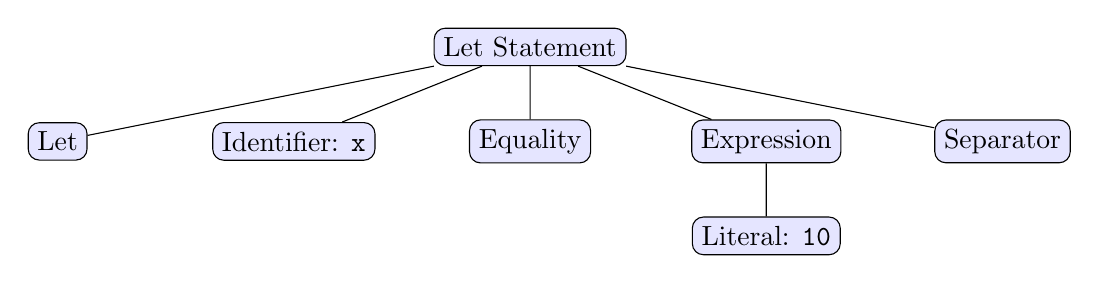
\begin{tikzpicture}[
                      level distance=1.2cm, sibling distance=3cm,
                      treenode/.style = {rectangle, rounded corners, draw, fill=blue!10, align=center}
                  ]
                  \node[treenode] {Let Statement}
                  child { node[treenode] {Let} }
                  child { node[treenode] {Identifier: \texttt{x}} }
                  child { node[treenode] {Equality} }
                  child { node[treenode] {Expression} child { node[treenode] {Literal: \texttt{10}} } }
                  child { node[treenode] {Separator} };
              \end{tikzpicture}
          \end{center}
          The AST captures the program structure but not yet its full meaning.

    \item[Semantic Analyses] This phase traverses the AST to check for semantic correctness,
          enforcing rules that syntax alone cannot capture. This includes \emph{type checking}
          (ensuring that operations are performed on compatible types), verifying that
          variables are declared before use, and resolving the scope of identifiers. During
          this pass, the compiler builds a \emph{symbol table} to store information about
          program identifiers, such as their type and location. The output is often a
          semantically validated and annotated AST.
\end{description}

The backend takes the validated representation from the frontend and generates the final target
code. This process is typically mediated by one or more \emph{Intermediate Representations} (IRs).
An IR is a representation of the program that is lower-level than the source AST but more abstract
than machine code.
%
The use of an IR is a powerful design principle that decouples the frontend from the backend,
reducing the implementation effort from a combinatorial \(M \times N\) to a more manageable
\(M + N\) components. This modularity allows an infrastructure like
\emph{LLVM}~\cite{DBLP:conf/cgo/LattnerA04} to support multiple source languages and hardware
architectures with a shared set of optimizations. In the context of a \dsl, this same
principle enables targeting multiple high-level languages like \Ci, \textsc{Ada}, or \Rust
from a single, common IR.
%
This backend process generally involves two main stages:
\begin{description}
    \item[Optimization] A compiler usually performs transformation passes on the IR to improve
          code performance. The \GRust compiler keeps this stage minimal, as it delegates the
          responsibility of optimization to the highly-advanced \Rust compiler, which operates
          on the generated code. This significantly reduces the implementation complexity of \GRust
          itself.

    \item[Code Generation] Finally, the IR is translated into the target language. In the
          context of \GRust, this stage consists of generating safe and idiomatic \Rust
          source code from the final IR.
\end{description}

The \GRust compiler is designed as a source-to-source translator that follows this approach. It
transforms \GRust source code through a series of dedicated IRs, ultimately generating safe \Rust
code. The subsequent sections detail the design of each of these internal passes.

\paragraph{Structure of the \GRust Compiler}

The \GRust compiler repository is organized as a \Rust \emph{workspace}, a structure that manages a
set of related crates. This modular design separates user-facing elements from the internal compiler
passes, promoting maintainability and clarity. The key crates are detailed below, grouped by their
role in the ecosystem, and illustrated in \Cref{fig:grust:implem:choices:architecture:compilo}.

\begin{figure}[ht!]
    \centering
    
\includegraphics[width=1\textwidth]{compiler_graph.pdf}
    \caption[Architecture of the \GRust compiler.]%
    {The architecture of the \GRust compiler, illustrating the key passes of the compilation
        pipeline from source code to executable.}
    \label{fig:grust:implem:choices:architecture:compilo}
\end{figure}

\subparagraph{User-Facing Crates}
These are the crates developers directly interact with.
\begin{itemize}
    \item \texttt{grust}: The primary, user-facing crate that serves as a facade, consolidating all
          necessary elements for development. It provides the \texttt{grust!} macro, re-exports the
          core and standard libraries (\texttt{grust\_core} and \texttt{grust\_std}), and
          bundles key external libraries such as \texttt{futures}, \texttt{tokio}, \texttt{tracing},
          and \texttt{rayon}. This is the only crate developers need to import.

    \item \texttt{grust-std}: This crate acts as the standard library for \GRust, offering a
          collection of pre-built elements. It includes common mathematical functions and numerical
          algorithms like integrators, which are designed to be compatible with the push-based
          execution model.\footnote{The correctness of time and memory-dependent components, such as
              integrators, is not guaranteed in a push-based system. Consequently, \GRust imposes a
              typing discipline to restrict their usage, a mechanism further explained and formalized in
              \Cref{sec:semantics:grsync:react_typing} of \Cref{cha:semantics}.}
\end{itemize}

\subparagraph{Runtime Support}
This crate provides essential definitions for the generated code.
\begin{itemize}
    \item \texttt{grust-core}: This crate defines the fundamental traits and types required by the
          generated code. This includes the \texttt{Component} trait, which all compiled components
          must implement (\Cref{sec:grust:implem:choices:sync}), and specialized stream types used
          for scheduling inputs and timers in services (\Cref{sec:grust:implem:choices:frp}).
\end{itemize}

\subparagraph{Compiler Infrastructure}
These crates form the foundation of the compilation.
\begin{itemize}
    \item \texttt{grust-proc}: This crate defines the \texttt{grust!} procedural macro. As required
          by \Rust, its manifest (\texttt{Cargo.toml})\footnote{The \texttt{Cargo.toml} file of a
              package is its \emph{manifest}, containing metadata used to compile the package.} is
          configured with \texttt{proc-macro = true}. Its library file, shown below, contains the
          entry point that passes the token stream to the main compiler logic.
          \begin{lstlisting}[language=Rust,numbers=none]
use compiler_top::{handle_tokens, TokenStream};
// The GRust compiler, implemented as a procedural macro.
#[proc_macro]
pub fn grust(tokens: TokenStream) -> TokenStream {
    handle_tokens(tokens)
}
\end{lstlisting}

    \item \texttt{compiler-top}: This crate orchestrates the compilation pipeline. It contains the
          function \texttt{handle\_tokens} that invokes the sequence of analyses and transformation
          passes on the input tokens and returns the generated \Rust code.

    \item \texttt{compiler-common}: A utility crate that defines shared data structures used across
          the entire compiler, including types for representing \GRust operations, error-reporting
          structures, keywords, and graph data structures.
\end{itemize}

\subparagraph{Compiler Passes and Intermediate Representations}
The translation is performed across three internal crates, each corresponding to a pass of
transformation and a specific IR.
\begin{itemize}
    \item \texttt{compiler-ir0}: This pass is responsible for parsing, transforming the raw token
          stream into an AST. The process is built upon the \texttt{syn} crate~\cite{syn_rust}, a
          parsing library. The parser is implemented by defining AST data structures that implement
          the \texttt{Parse} trait. This approach simplifies the development of a parser
          by turning the complex task of implementing a parsing algorithm (like
          LALR~\cite{DBLP:journals/toplas/DeRemerP82}) into the more manageable one of defining the shape of the
          expected code.

    \item \texttt{compiler-ir1}: This pass performs semantic analyses on the AST. This includes type
          checking (it is an implementation of the typing rules from \Cref{sec:grust:typing}),
          dependency graphs generation, causality analysis for components (this is a specific
          analysis that is detailed in \Cref{sec:grust:implem:choices:sync}), and other correctness
          checks and normalization processes. This pass enriches the AST with semantic information,
          preparing it for code generation.

    \item \texttt{compiler-ir2}: The final pass is responsible for code generation. It encodes
          the annotated AST into a target-agnostic IR. This IR models the high-level semantics of
          the program, representing components as state machines and services as import
          propagators.\footnote{This representation is abstract; at this stage, it could
              theoretically be used to generate \Ci or other languages.} The translation of this IR
          into \Rust code is then orchestrated by the \texttt{quote} crate~\cite{quote_rust}. Each
          element in the IR implements the \texttt{ToTokens} trait, which defines how it should be
          rendered as a stream of \Rust tokens. The \texttt{quote!} macro provides a template-like
          syntax that closely resembles the structure of the final \Rust code, making the
          code-generation logic highly readable and maintainable. For instance, the translation of a
          unary operation is defined as follows.
          \begin{lstlisting}[language=Rust]
// IR definition (`Box` is used for recursive types)
struct UnaryOperation { op: UnaryOp, expr: Box<Expression> }
// The implementation that generates Rust code
impl ToTokens for UnaryOperation {
    fn to_tokens(&self, tokens: &mut TokenStream) {
        let UnaryOperation { op, expr } = self;
        quote! { #op #expr }.to_tokens(tokens)
    }
}
\end{lstlisting}
          The code within the \texttt{quote!} macro directly mirrors the target \Rust syntax. The
          \texttt{\#op} and \texttt{\#expr} placeholders are interpolated, which recursively invokes
          the \texttt{ToTokens} implementation for the inner fields. This compositional approach
          allows the entire IR to be translated into a final token stream, which is then returned by
          the procedural macro.
\end{itemize}

The two following sections detail the compilation of the two sub-languages of \GRust, namely \GRSync
and \GRFRP.

\subsubsection{Compilation of \GRSync Functions and Components}
\label{sec:grust:implem:choices:sync}

This section describes the compilation for the two main constructs of the \GRSync
sub-language: functions and components.

\paragraph{Compilation targets}
While both are translated into \Rust code, their compilation targets and the challenges they present
are different.

The compilation of \GRSync functions is straightforward. As these functions are purely combinatorial
and stateless, they map directly to standard \Rust functions. The compiler's role is primarily to
perform semantic checks---such as verifying the correct usage of identifiers (ensuring that they do
not call components) and ensuring type consistency---before generating the equivalent, syntactically
correct \Rust function. Because those analyses are also performed on components, the detailed
explanation of the compilation will be focused on components.

The compilation of a \GRSync component produces three \Rust structs: one for inputs, one for
outputs, and one for the internal state. The state struct implements the \texttt{Component} trait,
which is defined in the \texttt{grust-core} library as follows.
\begin{lstlisting}[language=Rust]
pub trait Component {
    type Input;
    type Output;
    fn init() -> Self;
    fn step(&mut self, input: Self::Input) -> Self::Output;
}
\end{lstlisting}
The \texttt{Self} type refers to the type implementing the trait (the implementor), \texttt{self}
refers to an instance of \texttt{Self}, and \texttt{\&mut self} is a syntactic sugar for
\texttt{self: \&mut Self}.
%
The \texttt{Component} trait defines the framework for a synchronous, stateful computation.
The \texttt{init} function creates an instance of the component in its initial state. The
\texttt{step} function executes a single computational step: from a mutable reference to the current
state (\texttt{\&mut self}) and the current input, it produces the corresponding output, and updates
the state for the next step.
%
The \texttt{Input} and \texttt{Output} are associated types that an implementor of the trait must
specify. For a compiled \GRSync component, the generated state struct implements this trait,
providing the generated input and output structs as the concrete types for \texttt{Input} and
\texttt{Output}, respectively.

This translation exposes a paradigm mismatch. A \GRSync component is defined by a set of
unordered, declarative equations that specify relationships between dataflows. In contrast,
the generated \texttt{step} function must be an imperative, sequential block of code.
The primary challenge for the compiler is therefore to resolve the data dependencies
inherent in the component's equations, establish a valid partial order for their
execution, and synthesize a single, imperative \texttt{step} function that correctly
implements the component's semantics, formalized in \Cref{sec:semantics:grsync:opsem} of
\Cref{cha:semantics}.

\paragraph{Detailed Compilation Passes}
The compilation of a \GRSync component is a multi-stage process that transforms the
declarative, dataflow-oriented source code into an imperative \Rust state machine.
\Cref{fig:grust:implem:choices:sync:compilation} expands upon the general compiler
architecture from \Cref{fig:grust:implem:choices:architecture:compilo}, detailing the
specific analyses and transformation passes within the \texttt{compiler-ir1} crate that
are dedicated to \GRSync components.

\begin{figure}[ht!]
    \centering
    
\includegraphics[width=1\textwidth]{compiler_grsync.pdf}
    \caption[Compilation pipeline for \GRSync components.]%
    {The compilation pipeline for \GRSync components, illustrating the passes from source
        code to the \Rust tokens.}
    \label{fig:grust:implem:choices:sync:compilation}
\end{figure}

To illustrate this process, we will follow the compilation of a simple example: a \texttt{toggle}
component that flips a boolean state each time it receives a trigger event.

\begin{lstlisting}[language=GRust]
component toggle(trigger: unit?) -> (state: bool) {
    when {
        init => {state = false;}             // The initial state is `off'.
        trigger? => {state = !(last state);} // When triggered, flip the last state.
    }
}
\end{lstlisting}

\begin{enumerate}
    \item \textbf{Parsing:} The process begins by parsing the source text into an AST. This pass
          was previously explained in \Cref{sec:grust:implem:choices:architecture}. The AST for our
          \texttt{toggle} example is shown below.
          \begin{figure}[H]
              \centering
              
\includegraphics[width=0.8\textwidth]{grsync/ast.pdf}
              \caption[Parsed AST of a component.]%
              {Parsed AST for the \texttt{toggle} example.}
              \label{fig:grust:implem:choices:sync:ast}
          \end{figure}

    \item \textbf{Identifier Analysis:} The compiler traverses the AST to resolve all identifiers,
          replacing string-based names with unique IDs based on the scoping rules from
          \Cref{sec:grust:id_usage:grsync}. Information about each identifier is stored in a central
          \emph{symbol table}. Instantiations and declarations (differentiated by the scope of the
          identifiers they define) are referred to as `equations'.

          Symbol table after identifier analysis:
          \begin{center}
              \begin{tabular}{|lcl|}
                  \hline
                  0 & $\mapsto$ & component \{\texttt{toggle}\}                   \\
                  1 & $\mapsto$ & identifier \{\texttt{input}, \texttt{trigger}\} \\
                  2 & $\mapsto$ & identifier \{\texttt{output}, \texttt{state}\}  \\
                  \hline
              \end{tabular}
          \end{center}

          The AST is updated to use these unique IDs instead of names:
          \begin{figure}[H]
              \centering
              
\includegraphics[width=0.8\textwidth]{grsync/id_ast.pdf}
              \caption[Annotated AST of a component after the identifier analysis.]%
              {Annotated AST after the identifier analysis for the \texttt{toggle} example.}
              \label{fig:grust:implem:choices:sync:id_ast}
          \end{figure}

    \item \textbf{Type Analysis:} The compiler performs type checking according to the type system
          in \Cref{sec:grust:typing:grsync}. The types of all identifiers are verified. Once
          validated, this type information is added to the symbol table.

          Symbol table after type analysis:
          \begin{center}
              \begin{tabular}{|lcl|}
                  \hline
                  0 & $\mapsto$ & component \{\texttt{toggle}\}                                   \\
                  1 & $\mapsto$ & identifier \{\texttt{input}, \texttt{trigger}, \texttt{unit?}\} \\
                  2 & $\mapsto$ & identifier \{\texttt{output}, \texttt{state}, \texttt{bool}\}   \\
                  \hline
              \end{tabular}
          \end{center}

          The AST is updated to remove types:
          \begin{figure}[H]
              \centering
              
\includegraphics[width=0.8\textwidth]{grsync/ty_ast.pdf}
              \caption[Annotated AST of a component after the typing analysis.]%
              {Annotated AST after the typing analysis for the \texttt{toggle} example.}
              \label{fig:grust:implem:choices:sync:ty_ast}
          \end{figure}

          In addition to standard type checking, a sound implementation must also enforce the rules
          of the \emph{reactive type system}, which is formally detailed in
          \Cref{sec:semantics:grsync:react_typing} of \Cref{cha:semantics}. This system is crucial
          for guaranteeing that a component's behavior remains consistent when used within an
          asynchronous, event-driven \GRFRP service.

          The core challenge arises from constructs like the \kft{time} operator and untriggered
          \kft{last} memories. These can create \emph{continuous} flows, whose values change with
          every execution step, not just in response to input events. If not properly controlled,
          these flows can lead to non-compositional behavior, where a component's output depends on
          the rate of execution (\eg oversampling) rather than solely on its declared inputs.

          The reactive type system addresses this by classifying all flows as either
          \emph{continuous} or \emph{discrete}. It then enforces rules that prevent continuous flows
          from improperly influencing stateful computations. The soundness of this approach is
          formally established by the \emph{Oversampling Theorem}
          (\Cref{thm:semantics:grsync:theorems:oversampling}), which proves that well-typed programs
          are immune to such inconsistencies.

    \item \textbf{Causality Analysis:} This pass ensures that a component is computable by analyzing
          its data dependencies. The compiler constructs a \emph{dependency graph} where nodes
          represent the component's identifiers and edges represent the dataflows between them.

          Each edge is assigned a weight corresponding to its temporal delay.
          \begin{itemize}
              \item An \emph{instantaneous} dependency, such as in the expression \texttt{a + b},
                    has a weight of \texttt{0}.
              \item A \emph{delayed} dependency, introduced by the \kft{last} operator, has a
                    weight of \texttt{1}.
              \item For a \emph{component call}, the weight of a dependency from one of its inputs
                    to one of its outputs is computed from the dependency graph of the called
                    component. Specifically, it is the minimum possible sum of weights along any
                    simple path connecting that input to that output. This can result in weights
                    greater than \texttt{1}.
          \end{itemize}

          A component is defined as \emph{causal} if and only if this graph contains no cycles
          composed exclusively of \texttt{0}-weight edges. Such a cycle would represent a logical
          deadlock, where a computation depends on its result within the same logical instant.

          To verify this property, the compiler detects cycles in the subgraph of instantaneous
          dependencies using a topological sorting algorithm provided by the \texttt{petgraph}
          crate~\cite{petgraph_rust}. This algorithm returns a linear ordering of the nodes such
          that for every edge $x \rightarrow y$ within the graph, $x$ comes before $y$ in the
          ordering.
          %   The process is as follows:
          %   \begin{enumerate}
          %       \item For each node in the instantaneous graph, compute its \emph{in-degree} (the
          %             number of incoming edges).
          %       \item Initialize a queue with all nodes that have an in-degree of \texttt{0}.
          %       \item While the queue is not empty, dequeue a node and add it to an ordered list of
          %             computations. For each of its neighbors, decrement their in-degree. If a
          %             neighbor's in-degree becomes \texttt{0}, add it to the queue.
          %       \item If the final ordered list contains all nodes from the graph, no instantaneous
          %             cycle exists. If the list is smaller than the number of nodes, a cycle has been
          %             detected and the component is not causal.
          %   \end{enumerate}
          The absence of a cycle guarantees that a valid, sequential execution order exists for each
          step. This principle ensures the productivity of components in \Cref{thm:semantics:grsync:theorems:productivity}.

          \begin{multicols}{2}
              The dependency graph for \texttt{toggle}:
              \begin{center}
                  \begin{tikzpicture}
                      \node (trigger) [draw, circle] {1};
                      \node (state) [right= of trigger, draw, circle] {2};
                      \draw[arrow] (trigger) to [bend right=45]
                      node[midway, below]{\textcolor{gray}{0}} (state);
                      \draw[arrow] (state) to [loop right]
                      node[midway, right]{\textcolor{gray}{1}} (state);
                  \end{tikzpicture}
              \end{center}
              \newcolumn
              The output \texttt{state} (2) depends instantaneously on the input \texttt{trigger}
              (1) and on its own value with a delay of one step. Since the only cycle has a weight
              of \texttt{1}, the component is causal.
          \end{multicols}

    \item \textbf{Dead Code Analysis:} Using the dependency graph, the compiler also detects and
          warns about any variables that are defined but never used in the computation of an output.
          Here, all identifiers contribute to the output, so no dead code is found.

    \item \textbf{Normalization:} This pass simplifies the AST by rewriting complex constructs into
          a smaller subset of the language. This process, often called \emph{desugaring}, makes
          subsequent compiler passes, such as scheduling, much simpler as they only need to handle a
          limited set of language features. However, it is useful to perform the normalization after
          the analyses, in order to provide relevant errors to the \GRust programmer (\eg without
          identifiers generated by the compiler).
          %
          The main transformations are detailed below.

          \subparagraph{Transformation of \texttt{match} equations}
          To ensure that identifiers defined in \texttt{match} equations are accessible, they are
          transformed as \texttt{match} expressions. An equation like
          \begin{lstlisting}[language=GRust]
match color {
    Color { red, green, blue } if blue > 200 => { x = red; y = 2*x; }
    Color { red, green, blue } if blue > 100 => { x = green; y = 1; }
    Color { red, green, blue } => { x = blue; y = 0; }
}
\end{lstlisting}
          is transformed into a single equation where the \texttt{match} expression returns a tuple
          of the defined variables.
          \begin{lstlisting}[language=GRust]
(x, y) = match color {
    Color { red, green, blue } if blue > 200 => { x = red; y = 2*x; (x, y) }
    Color { red, green, blue } if blue > 100 => { x = green; y = 1; (x, y) }
    Color { red, green, blue } => { x = blue; y = 0; (x, y) }
}
\end{lstlisting}

          \subparagraph{Transformation of \texttt{when} equations}
          The most significant transformation is the conversion of \texttt{when} equations into
          \texttt{match} expressions.
          \begin{itemize}
              \item The \texttt{init} branch is separated and becomes a distinct initialization
                    equation.
              \item The remaining event-driven branches are compiled into a single \texttt{match}
                    expression over a tuple of all event inputs.
              \item An event pattern, like \texttt{trigger?}, becomes a \texttt{match} arm that
                    tests for the presence of a value using a compiler-internal \texttt{Some(..)}
                    pattern. This introduces a new local ID, corresponding to the event's unwrapped
                    value, stored in the symbol table.
              \item A rising edge pattern is implemented using a boolean state variable and a
                    \texttt{match} guard (\texttt{if ...}).
              \item A default branch is added (matching the wild card \texttt{\_}), corresponding
                    to the case where no event patterns are triggered.
              \item In each branch, the identifier created by the \texttt{when} equation that are
                    not defined in the branch get default values: a signal keeps its last value, and
                    an event is set to \texttt{None}.
              \item The \texttt{emit} operator (for event emissions) is replaced by a \texttt{Some}
                    wrapping.
          \end{itemize}
          For example, a complex \texttt{when} block with multiple event patterns:
          \begin{lstlisting}[language=GRust]
when {
    init         => {x = 0;}
    first_event? => {x = first_event; y = emit ();}
    edge         => {x = 0;}
    other_event? => {x = other_event;}
}
\end{lstlisting}
          is normalized into a set of equations that handles:
          1) the initialization of the \texttt{init} branch,
          2) the initialization and the logic of the rising edges, and
          3) finally uses a \texttt{match} over the events that implements the same priority as the
          initial \texttt{when} equation:
          \begin{lstlisting}[language=GRust]
init x = 0;                            // `init` branch
init test_edge = false;                // rising edge initialization
test_edge = edge && !(last test_edge); // rising edge detection
(x, y) = match (first_event, other_event) {
    (Some(first_event),_)  => { x = first_event; y = Some(()); (x, y) }
    (_,_) if test_edge     => { x = 0; y = None; (x, y) } // y is set to `None`
    (_, Some(other_event)) => { x = other_event; y = None; (x, y) }
    _                      => { x = last x; y = None; (x, y) } // default branch
}
\end{lstlisting}

          \subparagraph{Other simplifications}
          This pass also enforces other structural rules, such as ensuring that component calls
          only appear as the root of an expression and that their inputs are simple identifiers.

          \subparagraph{Applying normalization to the \texttt{toggle} example}
          For our running \texttt{toggle} example, the normalization pass transforms the
          \texttt{when} statement, adding a new local variable to the symbol table to hold the
          unwrapped value of the \texttt{trigger} event.

          Symbol table after normalization:
          \begin{center}
              \begin{tabular}{|lcl|}
                  \hline
                  0 & $\mapsto$ & component \{\texttt{toggle}\}                                   \\
                  1 & $\mapsto$ & identifier \{\texttt{input}, \texttt{trigger}, \texttt{unit?}\} \\
                  2 & $\mapsto$ & identifier \{\texttt{output}, \texttt{state}, \texttt{bool}\}   \\
                  3 & $\mapsto$ & identifier \{\texttt{local}, \texttt{trigger}, \texttt{unit}\}  \\
                  \hline
              \end{tabular}
          \end{center}

          The AST now reflects this basic structure, with the logic contained within an
          initialization and a \texttt{match} expression:
          \begin{figure}[H]
              \centering
              
\includegraphics[width=0.9\textwidth]{grsync/norm_ast.pdf}
              \caption[Annotated AST of a component after the normalization.]%
              {Annotated AST after the normalization for the \texttt{toggle} example.}
              \label{fig:grust:implem:choices:sync:norm_ast}
          \end{figure}

    \item \textbf{Memorization:} The compiler identifies all stateful elements: \texttt{last}
          memories and component applications. For each one of them, a memory field is allocated
          in the component's state, and a new identifier for accessing this memory is added to the
          symbol table. In the \texttt{toggle} example, this pass allocates a boolean field for
          \texttt{last state}, initialized to \texttt{false}.

          Symbol table after memorization:
          \begin{center}
              \begin{tabular}{|lcl|}
                  \hline
                  0 & $\mapsto$ & component \{\texttt{toggle}\}                                      \\
                  1 & $\mapsto$ & identifier \{\texttt{input}, \texttt{trigger}, \texttt{unit?}\}    \\
                  2 & $\mapsto$ & identifier \{\texttt{output}, \texttt{state}, \texttt{bool}\}      \\
                  3 & $\mapsto$ & identifier \{\texttt{local}, \texttt{trigger}, \texttt{unit}\}     \\
                  4 & $\mapsto$ & identifier \{\texttt{memory}, \texttt{mem\_state}, \texttt{bool}\} \\
                  \hline
              \end{tabular}
          \end{center}

          The AST is updated to replace \texttt{last} expressions with accesses to these
          new memory identifiers:
          \begin{figure}[H]
              \centering
              
\includegraphics[width=0.9\textwidth]{grsync/mem_ast.pdf}
              \caption[Annotated AST of a component after the memorization.]%
              {Annotated AST after the memorization for the \texttt{toggle} example.}
              \label{fig:grust:implem:choices:sync:mem_ast}
          \end{figure}

    \item \textbf{Inlining:}
          Inlining is a compilation pass that resolves certain feedback loops by replacing a
          component call with its internal equations. While a system of components might
          be proven causal at a high level, its structure can create a scheduling deadlock for the
          code generator. Inlining is crucial for resolving these cases, transforming a component
          that is logically sound but not directly compilable into one that is.

          Consider the following two components, which create a feedback loop:
          \begin{lstlisting}[language=GRust]
component apply_last(a: int) -> (b: int) {
    init b = 0; b = last a + 1;
}

component calling() -> (x: int) {
    x = apply_last(x);
}
\end{lstlisting}
          From a temporal perspective, this system is valid. The causality analysis can determine
          that the dependency of \texttt{x} on itself is not instantaneous but is delayed by one
          step (\via the \texttt{last a} inside \texttt{apply\_last}). The component is therefore
          causal.

          However, from a scheduling perspective, there is a deadlock. In the \texttt{calling}
          component, the equation \texttt{x = apply\_last(x)} creates a direct cyclic dependency at
          the level of the function call. To compute \texttt{x}, the compiler must first evaluate
          \texttt{apply\_last(x)}, which requires \texttt{x} as an input---a value that is not yet
          available within the current step.

          To break this scheduling deadlock, the compiler inlines \texttt{apply\_last} into
          \texttt{calling}. This transformation replaces the call with the actual equations of the
          callee, resulting in the following equivalent component:
          \begin{lstlisting}[language=GRust]
component calling() -> (x: int) {
    init x = 0; x = last x + 1;
}
\end{lstlisting}
          This transformed code makes the delayed feedback explicit: \texttt{x = last x + 1}. The
          compiler can now easily implement this logic using a single state variable that is read
          at the beginning of a step and updated at the end. The compilation is no longer blocked.

          Our running example, \texttt{toggle}, does not involve such inter-component feedback
          loops, so it does not require inlining.

    \item \textbf{Scheduling:} This pass orders the declarative equations of a component into an
          imperative sequence. It uses the topological order from the causality analysis to ensure
          every variable is computed before it is used within the \texttt{step} function.

    \item \textbf{State Machine Encoding:} In this pass, the scheduled and normalized representation
          is encoded into a target-agnostic Intermediate Representation (IR) that models a state
          machine. This IR serves as a high-level structure from which the final \Rust code will be
          generated, implementing the \texttt{Component} trait.

          The IR for a component defines several key parts:
          \begin{itemize}
              \item An \emph{Input Struct} and an \emph{Output Struct}, which model the component's
                    input and output into typed data structures.
              \item A \emph{State Struct}, whose fields correspond to the memory elements identified
                    during the memorization (\ie every use of the \texttt{last} operator and every
                    component call).
              \item An \emph{Initialization Function}, which models the \texttt{init} method of the
                    \texttt{Component} trait. Its role is to construct an initial instance of the
                    State Struct with the values derived from the component's \texttt{init}
                    statements.
              \item A \emph{Step Function}, which models the \texttt{step} method. Its body contains
                    the imperative sequence of statements produced by the scheduling pass. Input and
                    memory identifier accesses are specified. The Step Function also models the
                    state update and the returned outputs, collected into the Output Struct.
          \end{itemize}
          All identifiers and types are retrieved from the symbol table. Within the Step Function,
          accesses to input and to stateful variables are specified as so.

          The IR for the \texttt{toggle} component is shown below.
\end{enumerate}
\begin{figure}[H]
    \centering
    
\includegraphics[width=\textwidth]{grsync/ir.pdf}
    \caption[IR encoding of a component.]%
    {IR encoding of the \texttt{toggle} example.}
    \label{fig:grust:implem:choices:sync:ir}
\end{figure}

\paragraph{Generated \Rust code}
The last pass generates \Rust code from the IR resulting from the previously detailed passes.
This paragraph illustrates the kind of \Rust code is generated, first for functions, and then for
components.

\subparagraph{Functions}
\GRSync functions are purely functional, meaning that only the parsing, identifier usage, type
checking, and \Rust code generation stages are performed on those constructs, and the \Rust code
generation is strait forward.I
%
\Cref{lst:grust:implem:choices:sync:fun} is the code generated by the compilation of the
\texttt{safety\_distance} \GRSync function from the example in \Cref{fig:code_acc}.
It is basically th same function, but with \Rust keywords and types (\texttt{float} is encoded as
\texttt{f64}, and \texttt{int} as \texttt{i64}, as requested by \ampere).

\begin{lstlisting}[
      label=lst:grust:implem:choices:sync:fun,
      language=Rust,
      caption={[Generated \Rust code for a \GRust function.]%
      Generated code for the \texttt{safety\_distance} function from \Cref{fig:code_acc}.}, captionpos=b
]
fn safety_distance(sv_v: f64, fv_v: f64) -> f64 {
    let (rho, b_max) = (1.0f64, 0.6f64 * 9.81f64);
    let sv_d_stop = (sv_v * rho) + ((sv_v * sv_v) / (2.0f64 * b_max));
    let fv_d_stop = (fv_v * fv_v) / (2.0f64 * b_max);
    sv_d_stop - fv_d_stop
}
\end{lstlisting}

\subparagraph{Components}
The IR of a component, as previously explained, models a state machine. Following the illustrative
example in \Cref{fig:grust:implem:choices:sync:ir}, it contains: the Name of the
component, its Input Output and State structs, an Init function that gives initial values to the
fields of the State struct, and a step function that contains the Body (all the scheduled equations)
the Update of the State struct fields and the values to the fields of the Output struct.
The code to generate becomes straight forwards, it is a direct translation from this model to \Rust.

Using the \texttt{toggle} example, the generated code is \Cref{lst:grust:implem:choices:sync:codegen}.
\begin{lstlisting}[
      label=lst:grust:implem:choices:sync:codegen,
      language=Rust,
      caption={[Generated \Rust code for a \GRust component.]%
      Generated code for the \texttt{toggle} component.}, 
      captionpos=b
]
// All inputs of the `toggle` component.
struct ToggleInput { trigger: Option<()> }
// All outputs of the `toggle` component.
struct ToggleOutput { state: bool }
// State structure of `toggle` component.
struct ToggleState { mem_state: bool }
// Implementation of `Component` trait.
impl grust::core::Component for ToggleState {
    type Input = ToggleInput;
    type Output = ToggleOutput;
    fn init() -> ToggleState {
        ToggleState { mem_state: false }
    }
    fn step(&mut self, input: ToggleInput) -> ToggleOutput {
        let state = match input.trigger {
            Some(trigger) => {
                let state = !(self.mem_state);
                state
            }
            _ => {
                let state = self.mem_state;
                state
            }
        };
        (self.mem_state)* = state;
        ToggleOutput { state }
    }
}
\end{lstlisting}
The generated input, output and state structs of the \texttt{toggle} component are respectively
named \texttt{ToggleInput}, \texttt{ToggleOutput} and \texttt{ToggleState}, following the
convention: component name in camelcase (\texttt{Toggle} for the example), concatenated with the
type of the structure (\texttt{Input}, \texttt{Output} and \texttt{State}).
%
The body of the \texttt{init} function simply contains a \texttt{ToggleState} structure, initialized
as specified by the IR.
%
The \texttt{step} function takes as parameters the current inputs and a mutable reference to the
current state. It performs the computations specified by its Body in the IR, updates the state, and
returns the output. Therefore, the current state is never overwritten before being read.

As another example, \Cref{lst:grust:implem:choices:sync:comp} shows the generated \Rust code
corresponding to the \texttt{acc} component from \Cref{fig:code_acc}. The state \texttt{AccState},
in this case, only retains the internal state of the invoked subcomponent \texttt{derive} (of type
\texttt{DeriveState}). The \texttt{init} function, constructing the initial state, initializes
\texttt{derive} by calling its own \texttt{init} function, since it is a component thus its state
also implements the \texttt{Component} trait.

\begin{lstlisting}[
      label=lst:grust:implem:choices:sync:comp,
      language=Rust,
      caption={[Generated code for the Adaptive Cruise Control component.]%
        Generated code for the \texttt{acc} component from \Cref{fig:code_acc}.}, captionpos=b
]
// All inputs of the ACC component.
struct AccInput { c: bool, d: f64, s: f64, t: f64 }
// State structure of ACC component.
struct AccState { derive: DeriveState }
// Implementation of `Component` trait.
impl grust::core::Component for AccState {
    type Input = AccInput;
    type Output = f64;
    fn init() -> AccState {
        AccState { derive: DeriveState::init() }
    }
    fn step(&mut self, input: AccInput) -> f64 {
        let v = self.derive.step(DeriveInput { x: input.d, t: input.t });
        let (d_safe, b, fv_v) = match input.c {
            true => {
                let fv_v = input.s + v;
                let d_safe = safety_distance(input.s, fv_v);
                let b = (v * v) / (2.0f64 * (input.d - d_safe));
                (d_safe, b, fv_v)
            }
            false => {
                let b = 0.0f64;
                let (fv_v, d_safe) = (0.0f64, 0.0f64);
                (d_safe, b, fv_v)
            }
        };
        b
    }
}
\end{lstlisting}

In a \GRust program, components are instantiated by calls in services. The following section details
the compilation of those services and how they operate the state machine generated by the
compilation of components.

\subsubsection{Compilation of \GRFRP Services and \GReact Operations}
\label{sec:grust:implem:choices:frp}

This section describes the compilation of \GRFRP services and \GReact operations.

\paragraph{Compilation targets}

The compilation target for a service is a \emph{propagation machine} that combines
the efficiency of push-based execution with the predictability of pull-based scheduling.
It must be responsive to changes in its imports while respecting temporal constraints.
As established in \Cref{sec:grust:implem:design_principles:async_rust},
the compiler generates asynchronous \Rust code to realize this push-based execution model.

\subparagraph{Timestamps}
Time-dependent constructs, such as the \texttt{@[min, max]} service annotation and the \GReact
operations \kft{time} and \kft{timeout}, necessitate a model of time in the implementation.
Consequently, flows are represented as sequences of timestamped values: for a signal, a timestamped
value represents an update at a specific time; for an event, it represents an occurrence.
%
In a push-based execution implemented in asynchronous \Rust, the timestamped values of the imports
are \texttt{Future} values, and thus the imports are \texttt{Stream} of timestamped values.
%
A service thus consumes an import \texttt{Stream} of timestamped values and produces an export
\texttt{Stream} of timestamped values.

\subparagraph{Timer stream}
In addition to external changes, a service must handle internal timing constraints. Operations such
as \kft{timeout(e, T)}, which triggers an event if \texttt{e} does not occur within a given
duration, require a dedicated timer mechanism. Each timer corresponds to a specific time-dependent
operation or constraint.

All timers within a service are defined in a single enumeration. The service runtime manages these
timers through two streams: an incoming stream of timer expirations and an outgoing stream of timer
resets. A reset command cancels any pending timer of the same variant, preventing it from firing.

This mechanism is implemented by \texttt{timer\_stream}, a custom \Rust \texttt{Stream} provided by
the \texttt{grust-core} library. It transforms an input stream of timer resets into an output stream
of timer expirations. Internally, it uses an ordered queue to manage pending timers and a
\texttt{Sleep} future to wait for the next imminent deadline.

The implementation of its \texttt{poll\_next} method is crucial and operates in two stages. First,
it polls the incoming stream of timer resets, collecting all available reset commands and updating
the ordered queue. During this stage, it handles important corner cases: if a reset is for the timer
that the \texttt{Sleep} future is currently awaiting, or if a new timer's deadline is more imminent
than the current one, the active \texttt{Sleep} is aborted and the affected timer is rescheduled.
Second, once the reset stream is pending (\ie has no more items available at the moment), the method
polls the \texttt{Sleep} future. If the future has completed, it signifies that a timer has expired.
The method then yields a \texttt{Poll::Ready} containing the expired timer and its timestamp, and it
arms the \texttt{Sleep} future for the next most imminent timer in the queue. Otherwise, it returns
\texttt{Poll::Pending}.

Since a new reset for a timer variant replaces any pending one, the queue size is bounded by the
number of variants in the timer enumeration. This property guarantees bounded memory usage for the
timer mechanism at runtime.

\subparagraph{Priority Stream}
Service computations are triggered by two sources: changes to imports and timer expirations. These
two streams of changes must be merged and processed in a well-defined order to ensure deterministic
behavior. Specifically, the semantics of the \kft{time} operator requires that changes are
processed in strictly increasing order of their timestamps.

To enforce this ordering, the compiler uses a \texttt{prio\_stream}. This stream wrapper consumes an
unordered input stream and applies a priority function to yield items according to the specified
order. Internally, it is implemented using a bounded-size priority queue which efficiently maintains
items in a sorted sequence.

The implementation of its \texttt{poll\_next} method coordinates polling the input stream with
managing the internal queue. On each poll, it first attempts to pull all items from the underlying
input stream. If an item is available, it is inserted into the priority queue. The queue has a fixed
capacity, typically equal to the number of distinct event sources, to prevent unbounded memory
growth. If an item arrives when the queue is full, the stream considers this a critical runtime
failure and yields an error. This design choice prevents the silent loss of events, which is
unacceptable in high-integrity systems.

The stream yields an item from its internal queue only when the underlying input stream returns
\texttt{Poll::Pending}, ensuring that it has buffered all concurrently available events before
deciding which one has the highest priority. This strategy guarantees that the output is correctly
ordered, even when multiple events arrive in the same polling cycle. While the current
implementation primarily uses timestamps to order events, the priority function is generic, allowing
for future extensions such as ordering by event criticality.

\subparagraph{Service Structure}
A service is compiled into a main asynchronous \texttt{run} function. This function accepts an input
\texttt{Stream} of timestamped import changes and the initial values for all imported signals. It
returns an output \texttt{Stream} of timestamped export changes.

Internally, the \texttt{run} function orchestrates several components. It sets up asynchronous
channels for timer resets and for exported values. It merges the incoming import stream with the
\texttt{timer\_stream} and feeds the result into the \texttt{prio\_stream} for ordering. Finally, it
instantiates the service state and spawns a background task that loops over the ordered stream,
propagating each change through the service logic.

Execution begins by propagating the initial signal values to establish a valid initial state for all
dataflows within the service. After initialization, the main asynchronous loop begins. It awaits the
next change from the ordered input stream and dispatches to the appropriate handler based on the
source, as shown in the following pseudo-code (\Cref{lst:grust:implem:choices:frp:dispatch}).
\begin{lstlisting}[
    language=Rust,
    label=lst:grust:implem:choices:frp:dispatch,
    captionpos=bottom,
    caption={[Dispatch mechanism of the main asynchronous loop.]%
    Dispatch mechanism of the main asynchronous loop to differentiate the inputs.}
    ]
// The main asynchronous loop processes events from the ordered input stream.
while let Some(change) = ordered_input_stream.next().await {
    // The `Input` enum aggregates all external imports and internal timers.
    match change {
        // Case 1: An update from an imported flow: `speed`.
        Input::Speed { value, timestamp } => {
            service.propagate_speed(value, timestamp).await;
        }
        
        // Case 2: An update from another imported flow: `brake`.
        Input::Brake { value, timestamp } => {
            service.propagate_brake(value, timestamp).await;
        }
        
        // ... other import handlers
        
        // Case 3: A timer expiration.
        Input::Timer { kind, timestamp } => {
            // The specific timer is handled in a nested match.
            match kind {
                TimerVariant::TimeoutCheck => {
                    service.propagate_timeout_check(timestamp).await;
                }
                // ... other timer handlers
            }
        }
    }
}
\end{lstlisting}

To implement this pattern, a service is compiled into a \Rust module that encapsulates its state and
logic through several generated elements.
\begin{description}
    \item[Context Struct]
          The \emph{Context Struct} holds the memories needed for future computations. These values,
          such as the last value of a signal, correspond to the state defined in the operational
          semantics (\Cref{sec:semantics:grfrp:opsem} in \Cref{cha:semantics}). Each stored value is
          paired with a boolean flag to indicate whether it has been updated in the current
          execution step.

    \item[Input Storage Struct]
          The \emph{Input Storage Struct} implements the delay specified by the annotation
          \texttt{@[min, max]}. It buffers incoming changes that arrive during the
          service delay phase. This struct also detects and raises an error if a flow
          changes multiple times within this phase, which could signify a loss of information.
          With the bounded priority queue, this is the second firewall against event storms.

    \item[Service State Struct]
          The \emph{Service State Struct} aggregates the entire state of the service.
          It contains the individual states of all instantiated components, the sender ends
          of the output and timer-reset channels, the reference time for the \kft{time}
          operator, the context struct, a flag for the delay phase, and the input storage struct.

    \item[Initialization Function]
          An \emph{Initialization Function} is generated to construct the service state.
          It sets the initial reference time, initializes the context and component states,
          sets the initial delay status, and accepts the provided sinks for outputs and timer resets.

    \item[Message Handlers]
          A set of dedicated asynchronous \emph{Message Handlers} is generated, with one
          handler for each import and timer variant. Each handler is responsible for
          propagating a change from its corresponding source through the service logic.
\end{description}

\begin{figure}[ht!]
    \centering
    
\includegraphics[width=0.8\textwidth]{execution_acc_serv.png}
    \caption[Simplified diagram of the Adaptive Cruise Control generated code.]%
    {Simplified diagram of the generated code for the ACC service,
        illustrating the runtime architecture and dataflow execution.}
    \label{fig:grust:implem:grfrp:acc:serv}
\end{figure}

The compilation architecture is illustrated in \Cref{fig:grust:implem:grfrp:acc:serv}, which
presents a simplified diagram of the generated code for the ACC example from \Cref{fig:code_acc}.
The diagram shows the data flow from the external communication \texttt{Bus} through the generated
runtime elements. The \texttt{prio\_stream} and \texttt{timer\_stream} process inputs and timers,
ordering them and handling timer resets, as described previously. These ordered changes are then
processed by the \texttt{Interface}, which represents the dispatch mechanism of the main
asynchronous loop from \Cref{lst:grust:implem:choices:frp:dispatch}. For each incoming
change, this mechanism executes a \texttt{match} statement that calls the specific message handler
responsible for that input (\eg a change from \texttt{radar\_m} would call
\texttt{propagate\_radar\_m}).

This handler initiates the propagation of the new value through the service dataflow graph.
The \texttt{Service} block in the diagram represents this compiled logic and visualizes the
contents of the generated \emph{Service State Struct}, named \texttt{ACCService}. The
elements depicted within this block directly map to the fields of this struct and its nested
\emph{Context Struct}: the states of internal components (\eg \texttt{state\_acc}, shown
in red), the reference time for temporal operations (\texttt{begin}, in orange), and
intermediate memories (\eg \texttt{speed\_m\_s}, in gray) held in the \emph{Context Struct}.

The gray arrows depict the internal dataflow graph between operations. This graph is statically
determined at compile time and compiled into a single, loop-free imperative function. Executing this
function triggers the dependent computations and concludes by sending computed values to the output
channels. The function itself is largely synchronous; it only becomes asynchronous when it must
\texttt{await} a \texttt{send} operation on one of these channels. The role of temporal operators is
exemplified by the \kft{time} block. It is triggered by all changes and uses their timestamp with
the reference time (\texttt{begin}) to compute the elapsed time, which is then further propagated
(orange arrows). For clarity, the propagation logic for some elements, such as the service delay and
timeout handlers (\texttt{acc\_delay} and \texttt{acc\_timeout}), has been omitted. The results of
these computations are sent \via the \texttt{output\_stream} back to the bus, while any timer
modifications are sent to the \texttt{timer\_stream}.

\paragraph{Detailed Compilation Passes}
The compilation of a \GRFRP service is a multi-stage process that transforms the declarative,
dataflow-oriented source code into the asynchronous \Rust propagation machine described previously.
%
\Cref{fig:grust:implem:choices:frp:compilation} expands upon the general compiler
architecture from \Cref{fig:grust:implem:choices:architecture:compilo}, detailing the
specific analyses and transformation passes within the \texttt{compiler-ir1} crate that
are dedicated to \GRFRP services.

\begin{figure}[ht!]
    \centering
    
\includegraphics[width=1\textwidth]{compiler_grfrp.pdf}
    \caption[Compilation pipeline for \GRFRP services.]%
    {The compilation pipeline for \GRFRP services, illustrating the passes from source
        code to the \Rust tokens.}
    \label{fig:grust:implem:choices:frp:compilation}
\end{figure}

To illustrate this process, we will use the following \texttt{hazard\_light\_controller} service as
a running example. This service toggles the hazard lights upon a button press and includes an
automatic shut-off feature to prevent battery drain. The service relies on the \texttt{toggle}
component, whose own compilation was detailed in \Cref{sec:grust:implem:choices:sync}.

\begin{lstlisting}[language=GRust]
import event hazard_button_pressed: unit;
export signal hazard_lights_on: bool;

service hazard_light_controller {
    let event auto_off_trigger: unit = timeout(hazard_button_pressed, 300000);
    hazard_lights_on = toggle(
        merge(hazard_button_pressed, auto_off_trigger)
    );
}
\end{lstlisting}

\begin{enumerate}
    \item \textbf{Parsing:} The process begins by parsing the source text into an AST, as explained
          in \Cref{sec:grust:implem:choices:architecture}. The AST for the
          \texttt{hazard\_light\_controller} service is shown below.
          \begin{figure}[H]
              \centering
              
\includegraphics[width=\textwidth]{grfrp/ast.pdf}
              \caption[Parsed AST of a service.]%
              {Parsed AST for the \texttt{hazard\_light\_controller} example.}
              \label{fig:grust:implem:choices:frp:ast}
          \end{figure}

    \item \textbf{Identifier Analysis:} The compiler traverses the AST to resolve all identifiers
          and populates a symbol table. This pass is identical to the one described for \GRSync
          components in \Cref{sec:grust:implem:choices:sync}. The resulting symbol table for our
          example is shown below.

          \begin{center}
              \begin{tabular}{|lcl|}
                  \hline
                  0 & $\mapsto$ & component \{\texttt{toggle}\}                              \\
                  1 & $\mapsto$ & identifier \{\texttt{input}, \texttt{trigger}\}            \\
                  2 & $\mapsto$ & identifier \{\texttt{output}, \texttt{state}\}             \\
                  3 & $\mapsto$ & service \{\texttt{hazard\_light\_controller}\}             \\
                  4 & $\mapsto$ & flow \{\texttt{import}, \texttt{hazard\_button\_pressed}\} \\
                  5 & $\mapsto$ & flow \{\texttt{export}, \texttt{hazard\_lights\_on}\}      \\
                  6 & $\mapsto$ & flow \{\texttt{local}, \texttt{auto\_off\_trigger}\}       \\
                  \hline
              \end{tabular}
          \end{center}

          The AST is updated to use these unique IDs instead of names:
          \begin{figure}[H]
              \centering
              
\includegraphics[width=0.9\textwidth]{grfrp/id_ast.pdf}
              \caption[Annotated AST of a service after the identifier analysis.]%
              {Annotated AST after the identifier analysis for the \texttt{hazard\_light\_controller} example.}
              \label{fig:grust:implem:choices:frp:id_ast}
          \end{figure}

    \item \textbf{Type Analysis:} The compiler performs type checking according to the type system
          in \Cref{sec:grust:typing:grsync}, annotating the symbol table with type information for
          each identifier. The updated symbol table for our example is shown below.

          \begin{center}
              \begin{tabular}{|lcl|}
                  \hline
                  0 & $\mapsto$ & component \{\texttt{toggle}\}                                                    \\
                  1 & $\mapsto$ & identifier \{\texttt{input}, \texttt{trigger}, \texttt{unit?}\}                  \\
                  2 & $\mapsto$ & identifier \{\texttt{output}, \texttt{state}, \texttt{bool}\}                    \\
                  3 & $\mapsto$ & service \{\texttt{hazard\_light\_controller}\}                                   \\
                  4 & $\mapsto$ & flow \{\texttt{import}, \texttt{hazard\_button\_pressed}, \texttt{Event(unit)}\} \\
                  5 & $\mapsto$ & flow \{\texttt{export}, \texttt{hazard\_lights\_on}, \texttt{Signal(bool)}\}     \\
                  6 & $\mapsto$ & flow \{\texttt{local}, \texttt{auto\_off\_trigger}, \texttt{Event(unit)}\}       \\
                  \hline
              \end{tabular}
          \end{center}

          The AST is updated to remove types:
          \begin{figure}[H]
              \centering
              
\includegraphics[width=0.6\textwidth]{grfrp/ty_ast.pdf}
              \caption[Annotated AST of a service after the typing analysis.]%
              {Annotated AST after the typing analysis for the
                  \texttt{hazard\_light\_controller} example.}
              \label{fig:grust:implem:choices:frp:ty_ast}
          \end{figure}

          This pass must also enforce the rules of the \emph{reactive type system} for \GRFRP, which
          is formally detailed in \Cref{sec:semantics:grfrp:react_typing} of \Cref{cha:semantics}.
          This system is essential for ensuring that service behavior remains predictable and
          compositional in an event-driven, push-based execution model.

          The central challenge is managing the \kft{time} operator, which introduces a
          \emph{continuous} flow whose value changes at every execution step. In an event-driven
          system, this can lead to \emph{oversampling}---where a service is executed due to an
          unrelated input---causing time-dependent logic to produce inconsistent results.

          To prevent this, the reactive type system classifies all flows as either \emph{continuous}
          or \emph{discrete}. It enforces strict rules, for instance, by ensuring that the inputs
          and outputs of stateful components are discrete. This discipline guarantees that the
          behavior of a service is determined by its declared data dependencies, not by the
          arbitrary timing of its execution. The soundness of this approach is formally established
          by the \emph{Oversampling Theorem} (\Cref{thm:semantics:grfrp:theorems:oversampling}).

    \item \textbf{Normalization:} This pass simplifies the AST by rewriting complex statements into
          a series of simple, single-assignment equations where operations apply only to
          identifiers. It also makes internal mechanisms, such as timers, explicit. For our example,
          the nested call is unraveled by introducing an intermediate flow, \texttt{x}, for the
          output of the \kft{merge} operation. The \kft{timeout} operation is also normalized,
          making its 300,000ms duration an explicit timer definition, \texttt{t}.

          \begin{lstlisting}[language=GRust]
import event hazard_button_pressed: unit;
export signal hazard_lights_on: bool;

service hazard_light_controller {
    let timer t = 300000;
    let event auto_off_trigger: unit = timeout(hazard_button_pressed, t);
    let event x: unit = merge(hazard_button_pressed, auto_off_trigger);
    hazard_lights_on = toggle(x);
}
\end{lstlisting}
          This transformation adds the new identifiers for the timer \texttt{t} and the local flow
          \texttt{x} to the symbol table.

          \begin{center}
              \begin{tabular}{|lcl|}
                  \hline
                  0 & $\mapsto$ & component \{\texttt{toggle}\}                                                    \\
                  1 & $\mapsto$ & identifier \{\texttt{input}, \texttt{trigger}, \texttt{unit?}\}                  \\
                  2 & $\mapsto$ & identifier \{\texttt{output}, \texttt{state}, \texttt{bool}\}                    \\
                  7 & $\mapsto$ & identifier \{\texttt{local}, \texttt{trigger}, \texttt{unit}\}                   \\
                  3 & $\mapsto$ & service \{\texttt{hazard\_light\_controller}\}                                   \\
                  4 & $\mapsto$ & flow \{\texttt{import}, \texttt{hazard\_button\_pressed}, \texttt{Event(unit)}\} \\
                  5 & $\mapsto$ & flow \{\texttt{export}, \texttt{hazard\_lights\_on}, \texttt{Signal(bool)}\}     \\
                  6 & $\mapsto$ & flow \{\texttt{local}, \texttt{auto\_off\_trigger}, \texttt{Event(unit)}\}       \\
                  8 & $\mapsto$ & timer \{\texttt{t}, \texttt{300000}\}                                            \\
                  9 & $\mapsto$ & flow \{\texttt{local}, \texttt{x}, \texttt{Event(unit)}\}                        \\
                  \hline
              \end{tabular}
          \end{center}

          The AST now reflects this basic structure:
          \begin{figure}[H]
              \centering
              
\includegraphics[width=0.8\textwidth]{grfrp/norm_ast.pdf}
              \caption[Normalized AST of a service.]%
              {Normalized AST for the \texttt{hazard\_light\_controller} example.}
              \label{fig:grust:implem:choices:frp:norm_ast}
          \end{figure}

    \item \textbf{Dataflow Analysis:} This pass constructs a directed acyclic graph representing the
          data dependencies between all flows in the service. This graph is essential for
          determining the propagation logic. For any given input change, the compiler traverses this
          graph to identify the exact sequence of operations that must be executed.

          \begin{multicols}{2}
              The dependency graph for the service \texttt{hazard\_light\_controller}:
              \begin{center}
                  \begin{tikzpicture}
                      \node (t) [draw, circle, fill=red!10] at (360/5 * 1:1cm) {8};
                      \node (hlo) [draw, circle] at (360/5 * 2:1cm) {5};
                      \node (x) [draw, circle] at (360/5 * 3:1cm) {9};
                      \node (hbp) [draw, circle, fill=red!10] at (360/5 * 4:1cm) {4};
                      \node (aot) [draw, circle] at (360/5 * 5:1cm) {6};
                      \draw[arrow] (x)   to [bend left=36] (hlo);
                      \draw[arrow] (hbp) to [bend left=36] (x);
                      \draw[arrow] (aot) to (x);
                      \draw[arrow] (hbp) to [bend right=36] (aot);
                      \draw[arrow] (t) to [bend left=36] (aot);
                  \end{tikzpicture}
              \end{center}
              \newcolumn
              The nodes in red represent the primary inputs to the dataflow: the imported event
              \texttt{hazard\_button\_pressed} (4) and the explicit timer \texttt{t} (8). The graph
              shows how a change from these sources propagates through the \kft{timeout} (6),
              \kft{merge} (9), and \texttt{toggle} (5) operations.
          \end{multicols}

    \item \textbf{Propagation Machine Encoding:} In this pass, the declarative, dataflow-oriented
          service definition is encoded into a target-agnostic Intermediate Representation (IR) that
          models the asynchronous propagation machine. This IR serves as the high-level blueprint
          from which the final asynchronous \Rust \texttt{run} function and its associated data
          structures are generated.

          The IR for a service defines several key parts:
          \begin{itemize}
              \item An \emph{Interface Definition}, which lists all imported flows, exported flows,
                    and internal timers. This is used to generate the \texttt{Input},
                    \texttt{Output} and \texttt{Timer} enumerations for the service channels.

              \item A \emph{Service State Struct}, which contains the complete memory of the service.
                    This includes the \emph{Context Struct} (for intermediate flow values) and the
                    states of all instantiated \GRSync components.

              \item An \emph{Initialization Handler}, which defines the computations that run once
                    before the main service loop begins.

              \item A \emph{Collection of Input Handlers}, which models the core reactive logic.
                    For each possible input (imports and timers), the IR models a handler as a pair:
                    a \emph{trigger} identifying the input, and a loop-free \emph{instruction
                        sequence} that propagates the change through the dataflow graph.
          \end{itemize}
          The core of this pass is generating the instruction sequences for the input handlers.
          The encoding of the \kft{timeout} and \kft{merge} operations provides a detailed
          example of this process.

          \subparagraph{Encoding of \kft{timeout}}
          A \kft{timeout} operation is sensitive to two distinct triggers: the arrival of its
          source event (which resets its countdown) and the firing of its own internal timer (which
          produces its output). The compiler must therefore generate logic for both scenarios.
          \begin{description}
              \item[Triggered by Source Event]
                    When the active handler corresponds to the source event (\eg
                    \texttt{hazard\_button\_pressed}), the compiler's goal is to reset the
                    countdown. It generates a \texttt{ResetTimer} instruction for the associated
                    timer.

              \item[Triggered by Timer Event]
                    When the active handler corresponds to the internal timer, it means the source
                    event did not arrive in time. The compiler generates instructions for two
                    actions:
                    \begin{enumerate}
                        \item A \texttt{DefineEvent} instruction to create the output event (\eg
                              \texttt{auto\_off\_trigger}) with a unit value, making it present for
                              the rest of the propagation step.
                        \item A \texttt{ResetTimer} instruction to re-arm the timeout, ensuring it
                              will fire again after another interval if the source event remains
                              absent.
                    \end{enumerate}

              \item[Concurrency]
                    The algorithm correctly handles the case where both the source event and the
                    timer event could arrive in the same logical step. The semantics of
                    \kft{timeout} dictate that the source event's arrival takes precedence. The
                    compiler reflects this by generating a conditional instruction: if the source
                    event is present, only the reset logic is executed.

              \item[Initialization]
                    During service initialization, a \texttt{ResetTimer} instruction is also
                    generated to start the first countdown.
          \end{description}

          \subparagraph{Encoding of \kft{merge}}
          The \kft{merge} operator combines two event streams, giving priority to the first
          event if both occur simultaneously.
          \begin{description}
              \item[Priority Mechanism]
                    For an operation like \kft{merge(event\_1, event\_2)}, the compiler generates
                    a nested conditional instruction sequence using \texttt{IfActivated} blocks.
                    This structure enforces the priority rule: the check for \texttt{event\_2} is
                    performed only if \texttt{event\_1} is absent.

              \item[Instruction Generation]
                    The compiler uses the dataflow graph to generate the most efficient logic for
                    the active handler:
                    \begin{enumerate}
                        \item If the handler's trigger can only affect \texttt{event\_1}, the compiler
                              generates a simple, non-nested \texttt{IfActivated} block that only
                              checks for that event.
                        \item Likewise, if only \texttt{event\_2} can be present, it generates a
                              simple check for that event, guarded by a check for the absence of
                              \texttt{event\_1}.
                        \item If both events could potentially be present, it generates the full
                              nested conditional structure to correctly handle the priority.
                    \end{enumerate}
                    In all active branches, a \texttt{DefineEvent} instruction is generated to
                    create the output event with the value from the corresponding source.

              \item[Initialization]
                    During service initialization, no events are present by definition, so the
                    compiler correctly generates an empty instruction sequence for this operation.
          \end{description}
\end{enumerate}

\paragraph{Generated \Rust code}
The final pass generates \Rust code from the IR, materializing the asynchronous
propagation machine described previously. This paragraph illustrates the generated code
using the \texttt{hazard\_light\_controller} service as a running example. For conciseness
and clarity, the presented code snippets have been commented and edited by hand.

The compiler generates a \Rust module for each service, encapsulating its logic and state.
\Cref{lst:grust:implem:choices:frp:structs} shows the core data structures for the
\texttt{hazard\_light\_controller} service.
%
The \texttt{Context} struct holds the transient state for a single execution step,
tracking which flows have changed. The main \texttt{HazardLightControllerService} struct
contains the long-term state, including the state of the instantiated \texttt{toggle}
component, the reference time, and the sender ends of the output and timer channels.

\begin{lstlisting}[
    label=lst:grust:implem:choices:frp:structs,
    language=Rust,
    caption={[\Rust data structures generated by a \GRust service.]%
    Core data structures generated for the \texttt{hazard\_light\_controller} service.},
    captionpos=b
]
pub mod hazard_light_controller {
    // Context holds the state for a single propagation step.
    // Each field is a tuple: (value, has_changed_flag).
    pub struct Context {
        hazard_lights_on: (bool, bool),
    }
    // The main state for the service.
    pub struct HazardLightControllerService {
        // The reference time.
        begin: Instant,
        // The state of the instantiated `toggle` component.
        toggle: ToggleState,
        // The context for the current step.
        context: Context,
        // Sinks for sending outputs and resetting timers.
        output: Sender<Output>,
        timer: Sender<(Timer, Instant)>,
    }

    impl HazardLightControllerService {
        // Initializes the service state.
        pub fn init(
            begin: Instant,
            output: Sender<Output>,
            timer: Sender<(Timer, Instant)>
        ) -> Self {
            Self {
                begin,
                toggle: ToggleState::init(),
                context: Context::init(),
                output,
                timer,
            }
        }
        // This handler runs once to establish the initial state of all flows.
        pub async fn handle_init(&mut self) -> Result<(), SendError> {
            let instant: Instant = self.begin;
            // Initiate the timer `t` for the `timeout` operator.
            self.timer.send((Timer::T, instant)).await?;
            // Compute the initial output of the `toggle` component.
            let ToggleOutput { state: hazard_lights_on } = self.toggle.step(
                ToggleInput { trigger: None }
            );
            // Store the initial value in the context.
            self.context.hazard_lights_on.set(hazard_lights_on);
            // Send the initial exported value.
            self.output.send(
                Output::HazardLightsOn(hazard_lights_on, instant),
            ).await?;
            Ok(())
        }
        // A handler is generated for each import and timer.
        pub async fn handle_hazard_button_pressed(
            &mut self, instant: Instant, value: ()
        ) -> Result<(), SendError> { /* ... propagation logic ... */ }
        pub async fn handle_timer_t(
            &mut self, instant: Instant
        ) -> Result<(), SendError> { /* ... propagation logic ... */ }
    }
}
\end{lstlisting}

The core of the execution logic resides in the generated message handlers. These are
asynchronous \Rust functions that implement the dataflow propagation for a specific
input. \Cref{lst:grust:implem:choices:frp:handler} shows the handler for the
\texttt{hazard\_button\_pressed} input.
%
When this handler is invoked, it first resets the context and then executes the scheduled
sequence of operations. For the \kft{timeout} operation, it sends a reset command to
the timer channel. For the \kft{merge} operation, it evaluates its inputs according to
the priority rules. Finally, it calls the \texttt{step} function of the \texttt{toggle}
component and, if the output has changed, sends the new value to the output channel.

\begin{lstlisting}[
    label=lst:grust:implem:choices:frp:handler,
    language=Rust,
    caption={[\Rust input handler for a \GRust service.]%
    Handler for the \texttt{hazard\_button\_pressed} input.},
    captionpos=b
]
// This handler is called when the `hazard_button_pressed` event is received.
pub async fn handle_hazard_button_pressed(
    &mut self, instant: Instant, value: ()
) -> Result<(), SendError> {
    let hazard_button_pressed = Some(value);
    // 1. Reset the context for a new propagation step.
    self.context.reset();

    // 2. Handle the `timeout` operation: reset the timer.
    self.timer.send((Timer::T, instant)).await?;

    // 3. Handle the `merge` operation. Since `hazard_button_pressed` has priority,
    //    the output of the merge is the value of this input.
    let mut combined_trigger = None;
    if hazard_button_pressed.is_some() {
        combined_trigger = hazard_button_pressed;
    }

    // 4. If the combined trigger is present, step the `toggle` component.
    if combined_trigger.is_some() {
        let ToggleOutput { state: hazard_lights_on } = self.toggle.step(
            ToggleInput { trigger: combined_trigger }
        );
        self.context.hazard_lights_on.set(hazard_lights_on);
        // 5. Send the new state to the output channel if it has changed.
        if self.context.hazard_lights_on.is_new() {
            self.output.send(
                Output::HazardLightsOn(hazard_lights_on, instant)
            ).await?;
        }
    }

    Ok(())
}
\end{lstlisting}

Calls to service handlers are coordinated by a runtime. It is implemented in a \texttt{runtime}
module composed of several elements. Enumerations such as \texttt{Timer}, \texttt{Input}, and
\texttt{Output} represent all possible timers, inputs (imports and timers), and outputs,
respectively. The \texttt{Runtime} struct encapsulates the state of all services defined in the
\GRust program.
%
These are presented in \Cref{lst:grust:implem:choices:frp:runtime_mod}. For this example,
the runtime holds the state of the \texttt{hazard\_light\_controller} service, as it is
the only service in the program.

\begin{lstlisting}[
    label=lst:grust:implem:choices:frp:runtime_mod,
    language=Rust,
    caption={[Runtime architecture for a \GRust service.]%
    Runtime architecture for the running example.},
    captionpos=b
]
// Timers enumeration for all services.
pub enum Timer { T }
// Input messages enumeration for all services.
pub enum Input {
    HazardButtonPressed((), Instant),
    Timer(Timer, Instant),
}
// Output messages enumeration for all services.
pub enum Output { HazardLightsOn(bool, Instant) }
// Runtime state, containing all service states.
pub struct Runtime { hazard_light_controller: hlc::HazardLightControllerService }
// Initial values for imported signals (none in this example).
pub struct RuntimeInit { }
// Implementation of the Runtime async run loop.
impl Runtime { /* ... */ }
// Hazard Light Controller service module.
pub mod hlc { /* ... */ }
\end{lstlisting}

The \texttt{Runtime} struct implements a \texttt{run\_loop} asynchronous function
(\Cref{lst:grust:implem:choices:frp:run_loop}). This loop operates over a stream of input
messages. It first calls the initialization handler for each service, then repeatedly
awaits the next message from the stream and dispatches it to the appropriate service
handler based on its variant.

\begin{lstlisting}[
    label=lst:grust:implem:choices:frp:run_loop,
    language=Rust,
    caption={[Asynchronous run loop of the runtime for a \GRust service.]%
    Asynchronous run loop of the runtime for the running example.},
    captionpos=b
]
pub async fn run_loop(
    mut self,
    input: impl futures::Stream<Item = Input>,
    init_vals: RuntimeInit,
) -> Result<(), SendError> {
    futures::pin_mut!(input);
    let RuntimeInit { } = init_vals;
    // Initialize all services.
    self.hazard_light_controller.handle_init().await?;
    // Main dispatch loop.
    while let Some(input) = input.next().await {
        match input {
            Input::HazardButtonPressed(value, instant) =>
                self.hazard_light_controller
                    .handle_hazard_button_pressed(instant, value).await?,
            Input::Timer(Timer::T, instant) =>
                self.hazard_light_controller.handle_timer_t(instant).await?,
        }
    }
    Ok(())
}
\end{lstlisting}

The runtime is launched by a \texttt{run} function that sets up the execution environment,
as shown in \Cref{lst:grust:implem:choices:frp:run}. It takes an input stream of
timestamped updates from the data bus and returns an output stream of computed values.
%
The function creates asynchronous communication channels for outputs and timers. The
output stream returned to the caller is the receiver part of a channel, while its sender
is passed to the runtime. Similarly, a timer channel is created; its sender is used by
services to reset timers, and its receiver is consumed by the \texttt{timer\_stream}.
%
The function then employs the \texttt{timer\_stream} and \texttt{prio\_stream}, the two
core \GRust constructs detailed in \Cref{sec:grust:implem:choices:frp}. The
\texttt{timer\_stream} is responsible for managing all service timers, while the
\texttt{prio\_stream} merges the timer stream with the main input stream and reorders all
messages by increasing timestamp to ensure deterministic execution.
%
All channels and internal buffers are bounded, with capacities determined at compile
time to prevent unbounded memory usage. For example, the timer channel capacity is the
number of timer variants, allowing each timer to be reset once per step without
blocking. The output channel capacity is the number of exported flows. Similarly, the
internal buffer of the \texttt{prio\_stream} is sized to the total number of input
sources---the sum of imported flows and timer variants---ensuring it can handle a
worst-case scenario where all sources produce an event in the same polling cycle.
%
Finally, the runtime is instantiated and launched as an asynchronous task using
\texttt{tokio::spawn}.

A known limitation is that the \texttt{timer\_stream} currently depends on the
\texttt{sleep\_until} function from the \texttt{tokio} library. Consequently, the generated
code requires a \texttt{tokio}-compatible runtime. Making this component
backend-agnostic is a planned improvement. Such a change would be crucial for
portability, allowing \GRust to target diverse execution environments, from other
general-purpose runtimes like \texttt{async-std} to specialized \texttt{no\_std} runtimes
for embedded systems like \texttt{embassy}.

\begin{lstlisting}[
    label=lst:grust:implem:choices:frp:run,
    language=Rust,
    caption={[Main \texttt{run} function that launches a service.]%
    Main \texttt{run} function that launches the service task.},
    captionpos=b
]
// This function launches the service and returns a stream of its outputs.
pub fn run(
    begin: Instant,
    input_stream: impl Stream<Item = Input> + Send + 'static,
    init_signals: RuntimeInit,
) -> Receiver<Output> {
    const TIMERS_SIZE: usize = 1;
    const OUTPUT_SIZE: usize = 1;
    const MESSAGES_NB: usize = 2; // 1 import + 1 timer

    // 1. Create bounded asynchronous channels for outputs and timers.
    let (output_sink, output_stream) = channel(OUTPUT_SIZE);
    let (timers_sink, timers_stream) = channel(TIMERS_SIZE);

    // 2. Create the timer stream to manage timeouts.
    let timers_stream = timer_stream::<_, _, TIMERS_SIZE>(timers_stream)
        .map(|(timer, deadline)| Input::Timer(timer, deadline));

    // 3. Merge and order all input sources using the priority stream.
    let ordered_inputs = prio_stream::<_, _, MESSAGES_NB>(
        select(input_stream, timers_stream),
        Input::order, // Order by increasing timestamp
    );

    // 4. Spawn the main asynchronous task.
    let runtime = Runtime::new(begin, output_sink, timers_sink);
    tokio::spawn(async move {
        let result = runtime.run_loop(ordered_inputs, init_signals).await;
        assert!(result.is_ok(), "Runtime loop failed");
    });

    // 5. Return the receiver end of the output channel.
    output_stream
}
\end{lstlisting}

The compilation of the \texttt{hazard\_light\_controller} service demonstrates the core push-based
execution model. For services that include an \texttt{@[min, max]} timing annotation, the compiler
generates additional logic to handle input buffering and real-time deadlines. This annotation
introduces two timers: one for the \texttt{min} delay and one for the \texttt{max} timeout. The
service's main state struct is augmented with a boolean flag \texttt{delayed}, to track the delay
phase, and an \texttt{InputStore} struct to buffer incoming messages.

The logic within each message handler is then modified: if the service is still in its delay phase
(\ie \texttt{delayed} is \texttt{false}), the handler stores the incoming value in the
\texttt{InputStore} and asserts that no previous value is being overwritten. If the delay has
passed, it propagates the value immediately.

Two dedicated handlers manage the timing constraints.
\begin{description}
    \item[Delay Handler] Triggered by the \texttt{min} timer, this handler processes the buffered
          values. The current implementation uses a \emph{full propagation} strategy: it propagates
          all stored inputs through the dataflow graph, with conditionals on signal changes and
          event occurrences. This may be less efficient for large graphs due to repeated checks.
    \item[Timeout Handler] Triggered by the \texttt{max} timer, this handler ensures the service
          produces an output within a bounded time, even without new inputs. It forces a
          re-evaluation of the service's dataflows, effectively "pulling" a fresh output to meet the
          liveness guarantee.
\end{description}
Upon the propagation of any new input, both the delay and timeout timers are reset, restarting the
timing window. This dual-timer mechanism provides a robust framework for handling both input
buffering and real-time liveness guarantees.

\subsubsection{Compilation of \GReusot Specifications}
\label{sec:grust:implem:choices:greusot}

This section details the compilation of \GReusot specifications, which enables formal verification
of \GRust programs. The compilation process bridges the abstraction gap between the high-level
\GRust models and the \Creusot verifier, which operates on plain \Rust code.

\paragraph{Compilation targets}

The primary goal is to translate \GReusot contracts, written as \texttt{requires} and
\texttt{ensures} clauses, into corresponding \Creusot annotations on the generated \Rust code.
Verification is then performed by running \texttt{cargo creusot prove} on the crate containing the
generated code.

A central challenge in this process is managed by the design of \Creusot itself, which operates with
two distinct sets of types. First are the standard \emph{executable types} of \Rust, such as
\texttt{i64}, which are used for the actual computation and compiled into machine code. These types
have machine-level semantics, including fixed sizes and the potential for overflow. Second are the
parallel \emph{logical types}, such as \texttt{Int}, which are used exclusively within
specifications to model the mathematical representation of the program's data. For example,
\texttt{Int} represents an unbounded, mathematical integer that never overflows. The core task of
the verifier is to prove that operations on executable types correctly implement the desired
properties expressed using logical types.

For stateless \GRSync functions, the \GRust compiler's strategy is to generate two distinct but
related \Rust elements to manage this duality:
\begin{enumerate}
    \item A standard, executable \Rust function annotated with \Creusot attributes. These
          attributes contain the translated specifications, which refer to the \emph{logical
              interpretations} of the function's inputs and outputs.
    \item A parallel, non-executable \emph{logical function} inside a dedicated \texttt{logical}
          module. This function operates entirely within the mathematical domain of \Creusot and
          serves as a pure model of the computation for verification purposes.
\end{enumerate}
An additional \texttt{ensures} clause is generated for the executable function, asserting that the
logical interpretation of its result is equal to the output of the logical function. This formally
links the computational code to its logical model, guaranteeing that the executable code correctly
implements the verified logic.

Verifying components is fundamentally more complex due to their stateful nature. A specification on
a component applies to its generated \texttt{step} method, which has the signature
\texttt{step(\&mut self, input)}. The \texttt{self} parameter represents the component's internal
memory, which is an accumulation of its past execution.
%
A specification on \texttt{step} therefore acts as an \emph{inductive proof step}: assuming the
component is in a valid state, it proves that the next transition is correct. To make this reasoning
possible, a verifier needs a \emph{state invariant}---a property that holds true for the state at
the beginning of every step.
%
The current prototype of \GReusot does not yet provide a syntax for defining these state invariants.
Consequently, specifications on components are limited to properties that can be proven for a single
step \emph{without making any assumptions about the component's history}. This is feasible when the
desired property is a relationship between the current inputs and outputs, as shown in the
\texttt{acc} example in \Cref{lst:grust:implem:greusot:comp:spec}.

\paragraph{Augmented Compilation Passes}

The compilation of \GReusot specifications augments the existing \GRSync pipeline
(\Cref{sec:grust:implem:choices:sync}). The core logic of a function or component is processed as
previously described, while its specifications are handled by extended compiler passes.

\begin{enumerate}
    \item \textbf{Parsing:} The \texttt{compiler-ir0} pass is extended to parse the logical terms
          and the \texttt{requires} and \texttt{ensures} blocks associated with both functions and
          components, attaching them to the corresponding AST nodes.

    \item \textbf{Analyses:} During the \texttt{compiler-ir1} pass, the expressions within the
          specifications are analyzed for type correctness and identifier scope, similar to the
          analyses of the main function or component body.

    \item \textbf{Code Generation:} The \texttt{compiler-ir2} pass generates the final \Rust code.
          When it encounters a specified function or component, it performs four key actions:
          \begin{itemize}
              \item It translates the \GReusot contracts into \Creusot's
                    \texttt{\#[requires(...)]} and \texttt{\#[ensures(...)]} attributes,
                    placing them on the generated computational \Rust function (or
                    \texttt{step} method for a component). Inside these attributes,
                    variables are converted to their logical representation using the
                    \texttt{@} syntax of \Creusot.
              \item For functions, it generates a parallel function in a \texttt{logical}
                    module. This function has the same body but uses the logical types of
                    \Creusot (\eg \texttt{Int}) and is marked with \texttt{\#[logic]} and
                    \texttt{\#[open]} to make it accessible for verification.
              \item For functions, it adds a final \texttt{\#[ensures(...)]} attribute to
                    the computational function to assert its equivalence with the
                    generated logical function, ensuring the verified properties apply to
                    the compiled code.
              \item During the translation of contracts, any call to another specified function is
                    automatically converted into a call to that function's logical counterpart. This
                    is the key mechanism that enables compositional verification.
          \end{itemize}
\end{enumerate}

The following paragraphs illustrate this process for both functions and components, using the ACC
example from \Cref{sec:grust:example}. Since \Creusot does not yet support floating-point
arithmetic, the examples are adapted to use integers.

\paragraph{Compilation of Specifications on Functions}

For pure functions, the translation is direct. \Cref{lst:grust:implem:greusot:fun:spec} shows the
\texttt{safety\_distance} function extended with a \GReusot specification, defining preconditions on
vehicle speeds and postconditions on the computed distance.

\begin{lstlisting}[
      label=lst:grust:implem:greusot:fun:spec,
      language=GRust,
      caption={[\GReusot specification of a function.]%
      \GReusot specification of the \texttt{safety\_distance} function from
      \Cref{fig:code_acc}.}, captionpos=b
]
function safety_distance(sv_v: int, fv_v: int) -> int
  requires { 0 < sv_v && sv_v <= 50 }
  requires { 0 < fv_v && fv_v < sv_v && sv_v - fv_v <= 10 }
  ensures  { 0 < result && result < 150 }
{
  let (rho: int, b_max: int) = (1, 6);
  let sv_d_stop: int = sv_v*rho + sv_v^2/(2*b_max);
  let fv_d_stop: int = fv_v^2/(2*b_max);
  return sv_d_stop - fv_d_stop;
}
\end{lstlisting}

The corresponding generated code is shown in \Cref{lst:grust:implem:greusot:fun:codegen}. The
specifications are translated into \Creusot attributes. Within these attributes
(\Cref{line:grust:implem:choices:greusot:fun:convert}), the \texttt{@} operator converts the
computational inputs (\eg \texttt{sv\_v: i64}) to their logical form (\texttt{sv\_v@: Int}). The
compiler also generates the \texttt{logical::safety\_distance} function and an \texttt{ensures}
clause (\Cref{line:grust:implem:choices:greusot:fun:ensures:logical}) to link the computational and
logical versions.

\begin{lstlisting}[
      label=lst:grust:implem:greusot:fun:codegen,
      language=Rust,
      caption={[Generated code for the \GReusot specification of a function.]%
      Generated code for the \GReusot specification of the \texttt{safety\_distance}
      function from \Cref{lst:grust:implem:greusot:fun:spec}.},
      captionpos=b
]
#[requires(0 < sv_v@ && sv_v@ <= 50)] $\label{line:grust:implem:choices:greusot:fun:convert}$
#[requires(0 < fv_v@ && fv_v@ < sv_v@ && sv_v@ - fv_v@ <= 10)]
#[ensures(0 < result@ && result@ < 150)]
#[ensures(result@ == logical::safety_distance(sv_v@, fv_v@))] $\label{line:grust:implem:choices:greusot:fun:ensures:logical}$
pub fn safety_distance(sv_v: i64, fv_v: i64) -> i64 { $\label{line:grust:implem:choices:greusot:fun:i64}$
  let (rho, b_max) = (1i64, 6i64);
  let sv_d_stop = sv_v*rho + ((sv_v*sv_v) / (2*b_max));
  let fv_d_stop = (fv_v*fv_v) / (2*b_max);
  sv_d_stop - fv_d_stop
}
mod logical {
  #[open] #[logic]
  pub fn safety_distance(sv_v: Int, fv_v: Int) -> Int {
    let (rho, b_max) = (1, 6);
    let sv_d_stop = sv_v*rho + ((sv_v*sv_v) / (2*b_max));
    let fv_d_stop = (fv_v*fv_v) / (2*b_max);
    sv_d_stop - fv_d_stop
  }
}
\end{lstlisting}

\paragraph{Compilation of Specifications on Components}

As established, verifying components is more complex. A specification on a component applies to its
generated \texttt{step} method. \Cref{lst:grust:implem:greusot:comp:spec} shows the \texttt{acc}
component with a \GReusot specification that defines its safe operating conditions, relying on an
intermediate function, \texttt{compute\_braking}.

\begin{lstlisting}[
  label=lst:grust:implem:greusot:comp:spec,
  language=GRust,
  caption={[\GReusot specification of a component.]%
  \GReusot specification of the \texttt{acc} component from \Cref{fig:code_acc}.},
  captionpos=b
]
component acc(c: bool, d: int, s: int, v: int) -> (b: int)
  // radar detection limitation
  requires { 0 < d && d < 150 }
  // ACC scope of usage
  requires { c => (0 < s && s <= 50) && (0 < s+v && v < 0 && -v <= 10) }
  // there is enough distance to brake at maximum rate
  requires { c => d - safety_distance(s, s+v) > (v^2)/12 }
  // braking rate is in correct interval
  ensures  { 0 <= b && b <= 6 }
{
  match c {
    true => {
      b = compute_braking(d - d_safe, v);
      let d_safe: int = safety_distance(s, fv_v);
      let fv_v: int = s + v;
    }
    false => {
      b = 0;
      let (fv_v: int, d_safe: int) = (0, 0);
    }
  }
}
// Intermediate braking function to pass the proof
function compute_braking(d_grace: int, v: int) -> int
  requires { (0 < d_grace &&  d_grace < 150) && (v < 0 && -v <= 10) }
  requires { d_grace > (v^2)/12 }
  ensures  { 0 <= result && result <= 6 }
{
  return (v^2) / (2*d_grace);
}
\end{lstlisting}

The generated code for the \texttt{step} method is shown in
\Cref{lst:grust:implem:greusot:comp:codegen}. The component's inputs are accessed through the
\texttt{input} struct. The call to \texttt{safety\_distance} within the \texttt{requires} clause is
translated into a call to its logical counterpart, \texttt{logical::safety\_distance}
(\Cref{line:grust:implem:choices:greusot:comp:logical:call}), enabling compositional reasoning.
The specified property can be proven because it only relates current inputs to the current output.
The ability to define and use state invariants is a key area for future work.

\begin{lstlisting}[
  label=lst:grust:implem:greusot:comp:codegen,
  language=Rust,
  caption={[Generated code for the \GReusot specification of a component.]%
  Generated code for the \GReusot specification of the \texttt{acc} component from
  \Cref{lst:grust:implem:greusot:comp:spec}.}, captionpos=b
]
#[requires(input.d@ < 150)]
#[requires(input.c ==> (0 < input.s@ && input.s@ <= 50) &&
                       (0 < input.s@ + input.v@ && input.v@ < 0 && - input.v@ <= 10))]
#[requires(input.c ==> input.d@ - logical::safety_distance(input.s@, input.s@ + input.v@) $\label{line:grust:implem:choices:greusot:comp:logical:call}$
                        > (input.v@*input.v@) / 12)]
#[ensures(0 <= result@ && result@ <= 6)]
fn step(state: &mut AccState, input: AccInput) -> i64 {
  let (d_safe, b, fv_v) = match input.c {
    true => {
      let fv_v = input.s + input.v;
      let d_safe = safety_distance(input.s, fv_v);
      let b = compute_braking(input.d - d_safe, input.v);
      (d_safe, b, fv_v)
    }
    false => {
      let b = 0i64;
      let (fv_v, d_safe) = (0i64, 0i64);
      (d_safe, b, fv_v)
    }
  };
  b
}
#[requires((0 < d_grace@ && d_grace@ < 150) && (v@ < 0 && - v@ <= 10))]
#[requires(d_grace@ > (v@*v@) / 12)]
#[ensures(0 <= result@ && result@ <= 6)]
#[ensures(result@ == logical::compute_braking(d_grace@, v@))]
pub fn compute_braking(d_grace: i64, v: i64) -> i64 {
  (v*v) / (2i64*d_grace)
}
mod logical { $\label{line:grust:implem:choices:greusot:comp:logical:begin}$
  #[open] #[logic]
  pub fn compute_braking(d_grace: Int, v: Int) -> Int {
    (v*v) / (2*d_grace)
  }
} $\label{line:grust:implem:choices:greusot:comp:logical:end}$
\end{lstlisting}

This translation strategy seamlessly integrates formal verification into the \GRust development
workflow. It allows engineers to prove properties at the model level while ensuring they hold for
the generated, low-level \Rust code, laying the groundwork for more advanced, stateful verification
in the future.

\subsection{Conclusion: \iso Assessment and Future Work}
\label{sec:grust:implem:assessment_and_future}

This chapter detailed the architecture and implementation of the \GRust compiler, a prototype
engineered to bridge the gap between high-level modeling and the demands of modern automotive
software. We conclude by assessing this implementation against the \iso safety standard and
outlining the path toward industrial adoption.

\subsubsection{Assessment Against the \iso Standard}

The design choices for \GRust were guided by the requirements of the \iso standard. The resulting
implementation provides a robust foundation for developing high-integrity software, addressing the
key pillars of the standard.

\paragraph{Unambiguous Design and Traceability}
The standard mandates a clear, reviewable design with traceability from requirements to code. \GRust
addresses this through its two-level dataflow model. High-level system architecture is captured in
\GRFRP services, while reusable logic is encapsulated in \GRSync components. This structure provides
a readable and formal specification, simplifying safety audits by allowing requirements to be traced
to understandable modeling constructs rather than dense, low-level code.

\paragraph{Safe Implementation and Formal Verification}
The standard strongly recommends formal methods for high-\Asil systems. The \GRust toolchain
supports this through two core features. First, by compiling to safe \Rust, it leverages the borrow
checker to eliminate entire classes of memory and concurrency errors by construction. Second, the
\GReusot extension allows safety properties to be defined in the abstract \GRust model and formally
verified on the generated \Rust code, providing a concrete path to fulfilling verification
requirements.

\paragraph{Feasible Tool Qualification}
The implementation of \GRust as a source-to-source compiler (a procedural macro)
strategically minimizes the cost of tool qualification. Instead of qualifying an entire compiler,
the scope is reduced to the correctness of the translation from \GRust to \Rust. This design allows
\GRust to leverage qualified \Rust toolchains like \ferrocene, making industrial adoption a feasible
goal.

\paragraph{Summary Checklist}
\Cref{tab:iso26262_checklist} summarizes how the features of the \GRust implementation map to the
objectives of the \iso standard, demonstrating a design that is a practical tool engineered for a
safety-critical development process.

\begin{table}[ht!]
    \centering
    \begin{tabular}{p{0.25\textwidth} p{0.3\textwidth} p{0.4\textwidth}}
        \toprule
        \textbf{\iso Clause / Topic}                                                &
        \textbf{Objective / Requirement}                                            &
        \textbf{How \GRust Addresses the Requirement}                                 \\
        \midrule

        \textbf{Part 6-7:} \newline Software Architectural Design                   &
        Use a modular, hierarchical structure. Define interfaces and ensure properties
        like cohesion and loose coupling.                                           &
        \GRust enforces this \via its two-level structure: \GRFRP services for high-level
        architecture and \GRSync components for modular, reusable units with explicit
        input/output interfaces.                                                      \\
        \midrule

        \textbf{Part 6, Table 3:} \newline Use of Modelling                         &
        Use of modelling and semi-formal notations is highly recommended for ASIL C/D to
        ensure an unambiguous specification.                                        &
        \GRust is a formal, domain-specific modeling language. Its synchronous dataflow
        semantics provide an unambiguous foundation for system design, directly meeting
        this recommendation.                                                          \\
        \midrule

        \textbf{Part 6, Table 4:} \newline Use of a Suitable Language               &
        The language should enforce strong typing, have a well-defined syntax, and prevent
        unspecified behaviors.                                                      &
        \GRust has a formal grammar and strong typing. By compiling to \Rust, it leverages
        a language recognized for its suitability in safety-critical systems,
        inheriting its memory and thread safety guarantees.                           \\
        \midrule

        \textbf{Part 6-8:} \newline Unit Design and Implementation                  &
        Enforce coding guidelines, ensure traceability, and prevent runtime errors. &
        The declarative nature of \GRust serves as a high-level coding guideline. The
        compilation to safe \Rust prevents entire classes of runtime errors by
        construction.                                                                 \\
        \midrule

        \textbf{Part 6-9, Table 7:} \newline Software Unit Verification             &
        Use of formal methods to prove the absence of runtime errors is highly recommended
        for ASIL D.                                                                 &
        \GReusot allows developers to specify
        safety properties at the model level and formally verify them on the generated
        \Rust code, providing a direct path to compliance.                            \\
        \midrule

        \textbf{Part 8-11:} \newline Confidence in the Use of Software Tools        &
        The potential for the tool to introduce or fail to detect errors must be analyzed.
        Tool qualification is required.                                             &
        The implementation as a source-to-source compiler reduces the qualification scope
        to the translation step, leveraging the qualified \Rust toolchain.            \\
        \bottomrule
    \end{tabular}
    \caption[\iso Compliance Checklist.]%
    {\iso Compliance Checklist for \GRust.}
    \label{tab:iso26262_checklist}
\end{table}

\subsubsection{Usage and Future Work on \GRust}

The current prototype serves as a robust proof of concept. A program is compiled into a
\texttt{run} function that launches the asynchronous runtime. Users must manually wire the
input and output streams of this function to the broader system and provide initial
values for imported signals \via the \texttt{RuntimeInit} structure. This first
propagation step establishes a consistent initial state before any external event is
processed.

To transition \GRust from a research prototype to a practical tool for industrial
deployment, several enhancements should be implemented:

\begin{itemize}
    \item \textbf{Connector Library.} A library of reusable connectors will abstract away
          the manual wiring of streams, simplifying integration with existing \Rust code
          at \ampere and improving modularity.

    \item \textbf{Expressive Initialization.} The initialization of component memories is
          currently limited to constant values. Future work will explore allowing
          components to be initialized from the initial values of their inputs,
          making their startup behavior more flexible and expressive.

    \item \textbf{Backend-Agnostic Runtime.} The current implementation of the timer
          mechanism depends on \texttt{tokio}. Refactoring this element to be
          backend-agnostic is a crucial step to ensure portability, allowing \GRust to
          target diverse execution environments, from other general-purpose runtimes to
          specialized embedded schedulers.

    \item \textbf{Developer Tooling.} To improve productivity and aid system-level
          validation, complementary tools should be envisioned for visualizing dataflow
          dependencies, profiling system responsiveness, and simplifying debugging of the
          generated code.
\end{itemize}

Together, these developments will transform \GRust into a language that the automotive industry can
seamlessly integrate into its safety-critical workflows.

\subsubsection{Future Work on \GReusot}
\label{sec:grust:greusot:future}

Formal verification is a key requirement for high-\Asil systems. We developed \GReusot as a proof of
concept to demonstrate the feasibility of this approach in \GRust, strengthening its relevance in
the automotive domain. While successful as a prototype, several enhancements are needed to mature
\GReusot into a practical and usable tool. This section outlines a non-exhaustive list of these
improvements.

\paragraph{Improving Proof Guidance with Local Assertions}
Deductive verification often requires the programmer to provide intermediate hints, or lemmas, to
guide the SMT solvers toward a proof. As illustrated by the auxiliary function \verb|compute_braking|
(\Cref{lst:grust:implem:greusot:comp:spec}), these details can congest the program. A more
ergonomic approach would be to allow engineers to insert assertions directly on local variables
within a function or component body. In functions, these assertions would be placed at their point
of use. In components, where equations are unordered, they could be declared in a dedicated block.
This would allow developers to state intermediate properties without polluting the public signature.
The compiler would then translate these into \Creusot assertions, inserting them at the correct
point in the scheduled \texttt{step} function after the relevant variable has been computed.

\paragraph{Verifying Stateful Behavior with Compositional Invariants}
The most significant current limitation is the verification of stateful components. To reason about
a component's behavior over time, a verifier needs a \emph{state invariant}---a property that is
true of the component's memory at every step. The current prototype lacks a syntax for defining such
invariants.

Future work should introduce an \texttt{invariant} clause for components. For this to be truly
useful, the verification must be \emph{compositional}. The proof of a parent component's invariant
must be able to rely on the invariants of the components it instantiates. This would be compiled
into a set of inductive proof obligations:
\begin{itemize}
    \item \textbf{Base Case:} The invariant must be established by the \texttt{init} function. This
          translates to an \texttt{ensures} clause on \texttt{init}, guaranteeing the invariant
          holds for the component's own state and for the initial states of all its sub-components.
    \item \textbf{Inductive Step (Assumption):} The \texttt{step} function can assume the invariant
          holds for its own state and for the states of its sub-components \emph{before} the step.
          This translates to a \texttt{requires} clause on \texttt{step}.
    \item \textbf{Inductive Step (Preservation):} The \texttt{step} function must preserve the
          invariant for its own state and for the states of its sub-components \emph{after} the
          step. This translates to an \texttt{ensures} clause on \texttt{step}.
\end{itemize}
To make such invariants practical, this would also necessitate extending the \GRust language to
allow the \texttt{init} function to depend on the initial values of inputs, enabling the
establishment of meaningful initial conditions.

\paragraph{Compositional Verification of Component Calls}
A further challenge lies in handling component calls within a specification. Since each instance of
a component maintains its own private state, a call inside a contract raises a difficult question:
what state should be used for the verification? One option is to create a \emph{ghost} state for the
call, but this is of limited use as nothing is known about its history. Another is to call a logical
version of the \texttt{step} function on an existing state, but it is not clear how to identify the
correct state instance.

A more robust solution would be to draw inspiration from established model checkers like
\Kind~\cite{DBLP:conf/cav/ChampionMST16}, which uses $k$-induction to verify properties of stateful
\Lustre nodes. Integrating a similar technique into \Creusot would represent a significant research
effort, but it would provide a powerful and truly compositional method for verifying complex,
hierarchical \GRust models.


\section{Benchmarks}
\label{sec:grust:benchmarks}

\GRust is designed to bridge the gap between high-level, model-based design and the safety,
performance, and concurrency features of \Rust that are critical for modern \sdv architectures.
It achieves this by unifying a deterministic, synchronous paradigm with high-level constructs for
asynchronous, event-driven behavior. A comprehensive evaluation must therefore validate the
effectiveness of this hybrid approach. Accordingly, our assessment is structured into three parts,
each targeting a core contribution. The evaluations were conducted during two internships that I
proposed, and their results provide independent validation for the contributions of this thesis.

The first two parts of the evaluation stem from an academic internship, conducted by Dimitry Doche,
and focused on validating the core principles of \GRust.
%
First, to assess the performance of the synchronous kernel, a quantitative analysis compares the
runtime efficiency of code generated by \GRust against that of established \Lustre compilers.
%
Second, to demonstrate improvements in design clarity, a qualitative case study contrasts a
high-level \GRust model of a complex concurrent system with its conventional low-level \Ci
implementation. Together, these results establish the performance and expressive power of the
language in a controlled academic setting.

The third and final part of our assessment demonstrates the practical applicability of \GRust for
\sdv development. This was the focus of an industrial internship at \ampere, conducted by Matthieu
Massif, which involved reimplementing existing industrial services in \GRust. The code metrics and
performance of these services were then compared on target hardware against the original,
handwritten asynchronous \Rust versions. A key outcome of this effort was the development of a
complete compilation and deployment toolchain, proving the integration of \GRust into a real-world
engineering workflow. These findings provide compelling evidence for the industrial viability of
\GRust, showing that it can be effectively integrated into the \Rust ecosystem at \ampere to
simplify the development of complex automotive software.

\subsection{\GRSync Performance Evaluation}
\label{sec:grust:benchmarks:compare_grsync}

%% Benchmark framework
This first evaluation assesses the performance of the synchronous kernel of \GRust,
\GRSync. To ensure a fair and direct comparison, we focus on purely synchronous systems,
which allows us to benchmark against established academic \Lustre compilers:
\Heptagon~\cite{heptagon}, \LustreC~\cite{lustrec}, and \Velus~\cite{velus}.
%% Goal: show that GSync is performant
The goal of this evaluation is to show that binaries generated by \GRSync for synchronous systems
relevant to our context are comparable behavior-wise and performance-wise to that of a
\Lustre-specific compiler. We propose to do so by comparing the run time of the binaries generated
by the compilers on a few realistic systems, using a series of 100,000 steps without interruption%
---meaning step $n+1$ starts as soon as step $n$ is over.

\subsubsection{Benchmark Tooling}
\label{sec:grust:benchmarks:compare_grsync:tools}

As part of the \GRust project, two key tools were developed by Adrien Champion in order to conduct
this evaluation: a \Lustre front-end for the \GRust compiler and a specialized benchmarking utility.
They are described in this section.

%% GLustre: Lustre => GRSync
\paragraph{\GLustre front-end}
To make \GRSync fit in this evaluation, we used a front-end for the \GRust compiler called
\GLustre that supports an expressive enough subset of the \Lustre language. It
front-end parses a \Lustre file, transpiles it to \GRSync, compiles the resulting file to \Rust code
and finally compiles the \Rust code. We thus obtain a binary for each of the \Lustre systems we want
to compare with.

%% Benchmark tool
\paragraph{\BenchIt tool}
To properly run the evaluation, we used \BenchIt, a tool specialized for
benchmarking synchronous systems by efficiently feeding them a large number of inputs and measuring
the time they take to produce the same number of step-outputs. Benchmarks are given as a \Lustre
file \texttt{<file>.lus} and an inputs file \texttt{<file>.toml} specifying a trace of inputs.
For a given benchmark, \BenchIt compares \Lustre compilers by: compiling the system with each
compiler to obtain a binary, pre-processing the inputs for each binary (they all have specific input
formats), measuring the time they take to produce all their step-outputs, and logging the run
times after confirming the traces of step-outputs.
Currently, \BenchIt supports the following compilers: \Heptagon, \GLustre, \LustreC, and \Velus.

Most \Lustre compilers produce a binary that starts with an initialization phase that dynamically
allocates all the memory it will need once it actually starts. We ignore the initialization phase
by waiting 500 milliseconds between starting the binaries and providing step-inputs, and
measure only the run time after we start feeding the inputs.

\BenchIt is also able to generate traces of random inputs for \Lustre systems. Ideally we would
want large, \emph{realistic} traces of inputs, but such traces are rarely available and
quite difficult to generate for embedded systems, usually requiring a complex, often
proprietary, simulation environment.

\subsubsection{Selected Systems}
\label{sec:grust:benchmarks:compare_grsync:selected_systems}

Given our industrial context, we are interested in reasonably realistic, ideally semi-industrial
systems. Also, we want the computation steps to be relatively expensive to lower the impact of the
low-level details specific to each compiler, such as the different ways the resulting binaries read
(write) their inputs (outputs).
%
For our evaluation, we selected several systems with increasing complexity that are presented below.
As \Lustre compilers have a tendency to differ in the \Lustre subset they support (state machines,
custom types, clocks, \etc), we had to rewrite and select the systems in the intersection of the
features and syntax accepted by all compilers to make sure all compilers work on the exact same
\Lustre source files.

\paragraph{Pololu}
%% Pololu %%
The \href{https://www.pololu.com/docs/0J83}{\pololu} is a small mobile platform designed for
educational purposes. It is controlled by an Arduino-type board, with reflectance sensors that
measure the grayscale intensity of the ground to the left, center, and right of the robot. Dimitry
Doche has implemented in \Lustre a simple controller that allows the robot to follow a dark line (by
comparing the measured grayscale to the expected grayscale of the line). As a sanity check, we have
embedded the \Ci code compiled from \Lustre: the controller step function is called in a \Ci
interface that connect the hardware to the controller. We computed the position of the robot
approximated from the speed of the wheels produced by the compilers on a randomly generated trace of
inputs. The results in \Cref{fig:grust:benchmarks:compare_grsync:selected_systems:pololu} confirm
that the \GLustre binary behaves consistently with the other three compilers, as shown by the
superposition of the four trajectories.

\begin{figure}[ht!]
    \centering
    
\includegraphics[width=0.6\textwidth]{trajectory_comparison_better.png}
    \caption[Positions of the Pololu.]%
    {Positions of the Pololu computed from one input trace, generated by the \Lustre
        compilers (\Heptagon, \LustreC, \Velus, and \GLustre) in comparison with the position
        computed by the robot.}
    \label{fig:grust:benchmarks:compare_grsync:selected_systems:pololu}
\end{figure}

\paragraph{Crazyflie}
%% Crazyflie %%
The \href{https://www.bitcraze.io/products/crazyflie-2-1-plus/}{\crazyflie} is a quadcopter drone
shipping with an open source development platform. We are interested in its Kalman filter, a
statistics estimator that uses sensor measurements over time to compute an estimation of the current
state. The original implementation is provided as \Ci code in the
firmware~\cite{DBLP:conf/icra/MullerHD15,MuellerCovariance2016}.%
\footnote{
    The code is available at
    \url{https://github.com/bitcraze/crazyflie-firmware/blob/master/src/modules/src/estimator/estimator_kalman.c}.
}
Dimitry Doche, assisted by Basile Pesin and Timothy Bourke (who have reimplemented the PID
controller of the \crazyflie in \Velus), translated the core of the estimator into the
\Lustre dialect of \Heptagon, which supports arrays
and composite data types. The resulting program contains approximately 1,000 lines of code or
35,000 tokens, excluding comments. As a sanity check, we verified that the resulting estimator and
the initial firmware \Ci code was producing the same outputs using a real input trace. The trace
was reconstructed by concatenating data from multiple \crazyflie drone flights. Sensor measurements
were obtained \via radio transmission, but due to bandwidth limitations, it was not possible to log
the entire input stream at once. We then transpiled this program into a simpler \Lustre variant
compatible with all compilers, which involved inlining arrays and structures. This significantly
increased the number of tokens (175,000) and of lines of code (15,000). We verified that all four
compilers produce identical output traces for several input traces of 100,000 steps.

\paragraph{TCM}
%% TCM %%
The \emph{Transport Class Model} (TCM) is a control system for a generic, mid-size, twin-engine,
commercial transport-class aircraft. It was originally developed by \textsc{NASA} Langley in
\Simulink~\cite{tcmOriginal}. It was later translated to \Lustre and equipped with a full formal
specification based on the \emph{Federal Aviation Regulations}~\cite{tcmCocospec}.%
\footnote{
    Code available at
    \href{https://github.com/kind2-mc/cocospec_tcm_experiments/tree/3b0834704e8434f1da08e45f79f129330faca6fc/systems}
    {https://github.com/kind2-mc/cocospec\_tcm\_experiments}.
}
As a semi-industrial system, it is an ideal candidate to evaluate the performance of synchronous
systems compiled by \GRust.

\paragraph{Kind~2 benches}
%% kind2 benches %%
Next, we ran our evaluation on approximately 200 \Lustre programs from the benchmark suite of the
Kind~2 model-checker~\cite{DBLP:conf/cav/ChampionMST16} (those included in the subset of \Lustre
that we consider for our comparison). Even though several of these systems are rather small, leaving
not much room for improvement, \GLustre shows suspiciously good performance compared to other
\Lustre compilers. To investigate this, we added a control benchmark, \texttt{in-out.lus}, which
takes several inputs and simply outputs the same constant at each step. Since \GLustre remains
significantly faster on this benchmark, we infer that the performance difference is not only
explained by the way \GLustre compiles the systems, but rather most likely influenced by low-level
aspects of the \Ci and \Rust runtimes, such as input scanning and output printing.

\subsubsection{Evaluation and Discussion}

\begin{figure}[ht!]
    \centering
    \begin{subfigure}{1\textwidth}
        \centering
        \begin{longtable}[c]{|lcc | c | c | c | c |}
            \hline
                                       &       &     & in-out & Pololu & TCM    & Crazyflie \\\hline\hline
            \multirow{2}{*}{\GRSync}   & Mean  & (s) & 0.1445 & 0.126  & 0.2466 & 0.72      \\
                                       & $\pm$ & (s) & 0.0003 & 0.002  & 0.0005 & 0.03      \\\hline
            \multirow{2}{*}{\Heptagon} & Mean  & (s) & 0.336  & 0.233  & 0.5871 & 2.15      \\
                                       & $\pm$ & (s) & 0.002  & 0.003  & 0.0006 & 0.06      \\\hline
            \multirow{2}{*}{\LustreC}  & Mean  & (s) & 0.4454 & 0.247  & 0.615  & 2.54      \\
                                       & $\pm$ & (s) & 0.0004 & 0.004  & 0.002  & 0.07      \\\hline
            \multirow{2}{*}{\Velus}    & Mean  & (s) & 0.342  & 0.231  & 0.5890 & 2.16      \\
                                       & $\pm$ & (s) & 0.003  & 0.003  & 0.0003 & 0.06      \\\hline
        \end{longtable}
        \caption[Comparison of execution time.]%
        {Comparison of execution time (in seconds) for the \texttt{in-out.lus}, Pololu, TCM,
            and \crazyflie systems.}
        \label{table:grust:benchmarks:compare_grsync:selected_systems:exec-time:others}
    \end{subfigure}

    \begin{subfigure}[b]{1\textwidth}
        \centering
        
\includegraphics[width=0.6\textwidth]{scatter_grust_comparaison_better.png}
        \caption[Comparison of execution time for the Kind~2 benches.]%
        {Comparison of execution time for the Kind~2 benches.}
        \label{fig:grust:benchmarks:compare_grsync:selected_systems:exec-time:kind2}
    \end{subfigure}
    \caption[Execution times for codes from \GRSync and academic compilers.]%
    {Combined comparisons of execution time on the different selected systems with input traces of
        100,000 steps, running each benchmark between 10 and 100 times.}
    \label{fig:grust:benchmarks:compare_grsync:selected_systems:exec-time}
\end{figure}

The performance evaluation, conducted by Dimitry Doche with assistance from Christophe Garion,
measured the execution time of the selected systems. The results are presented in
\Cref{fig:grust:benchmarks:compare_grsync:selected_systems:exec-time}. Each system was executed on
randomly generated input traces of 100,000 steps, and each benchmark was run between 10 and 100
times to ensure stable measurements.%
\footnote{
    The evaluation was performed on an Asus Zenbook 14 equipped with an AMD Ryzen 7 8840HS processor
    running Manjaro Linux.
}
We verified that all compilers produced equivalent output traces for each system, with the exception
of integer overflows, since \LustreC relies on 32-bit integers while the other compilers use 64-bit
integers.

\paragraph{Results}
The results for the evaluation on the bigger systems, detailed in
\Cref{table:grust:benchmarks:compare_grsync:selected_systems:exec-time:others}, show that \GRSync
(\via the \GLustre front-end) consistently outperforms the other compilers. For the most complex
systems, the TCM and the Kalman filter of the \crazyflie, the code generated by \GRSync runs two to
three times faster than the code from the next fastest compiler.

This trend is confirmed by the evaluation on the Kind~2 benchmark suite, illustrated in
\Cref{fig:grust:benchmarks:compare_grsync:selected_systems:exec-time:kind2}. The scatter plot
compares the execution time of \GRSync ($y$-axis) against the other compilers ($x$-axis) on a
logarithmic scale. To each point corresponds a benchmark program from Kind~2. A point below the main
diagonal ($y=x$) indicates that \GRSync is faster (the execution time of the \GRSync version
is smaller than the compared one). All the 200 benchmarks lie well below this diagonal,
demonstrating that the performance advantage \emph{of the toolchain of \GRSync} is consistent across
a wide variety of programs, not just a few large examples. This performance in suspiciously good,
these systems are rather small which leaves not much room for improvement.

The \texttt{in-out.lus} benchmark, which performs minimal computation, acts as a control to isolate
framework overhead. Even here, \GRSync is more than twice as fast as its counterparts
(\cf \Cref{table:grust:benchmarks:compare_grsync:selected_systems:exec-time:others}).

\paragraph{Analysis}
Even though the \GRSync toolchain is faster according to this evaluation, we \emph{do not claim}
that this is due to the way \GRSync compiles synchronous systems. As steps are often measured in
milliseconds, the low-level, \Ci/\Rust-specific details of scanning and parsing inputs, printing
outputs, operations on primitive types, \etc can become significant. This is highlighted by the
\texttt{in-out.lus} file, that operates as a scientific control; the evaluation of all the compilers
using this file showed a reduction of 200 milliseconds of the execution time for the code generated
by \GRSync.

However we \emph{do claim} that this evaluation shows that the synchronous part of \GRust and its
compilation framework relying on \Rust are competitive relative to state-of-the-art academic tools
that are specialized in `\Lustre to \Ci' compilation, despite \GRust targets a much richer language.

\subsection{Evaluation of the Design of a UAV with \GRust}
\label{sec:grust:benchmarks:eval_grust_design}

To demonstrate the benefits of using \GRust as a high-level modeling tool, we present a case study
centered on the Kalman filter from the state estimator of the \crazyflie UAV~\cite{crazyflie-fm},
described previously.

\paragraph{The original Kalman filter}
The original implements an adapted
\href{https://github.com/bitcraze/crazyflie-firmware/blob/b9d676aa3544b68eea17d11b0fbec437da909878/src/modules/src/kalman_core/kalman_core.c}
{Kalman filter}, which updates the estimated state of the drone based on incoming sensor
measurements~\cite{DBLP:conf/icra/MullerHD15,MuellerCovariance2016}.%
\footnote{
    Each important function of the estimator is referred with a link to the \Ci functions of the
    \crazyflie firmware.
}

The global algorithm of the stabilizer proceeds the following computations:
\begin{enumerate}
    \item \textbf{Reset:} The estimated state is reverted to its initial values upon system
          initialization or when a reset command is received.
    \item \textbf{Prediction:} The last estimated state is given to the physical model to
          \href{https://github.com/bitcraze/crazyflie-firmware/blob/b9d676aa3544b68eea17d11b0fbec437da909878/src/modules/src/kalman_core/kalman_core.c#L744C1-L791C2}
          {predict} the current state.
    \item \textbf{Transformation:} \href{https://github.com/bitcraze/crazyflie-firmware/blob/b9d676aa3544b68eea17d11b0fbec437da909878/src/modules/src/kalman_core/kalman_core.c#L613C1-L619C2}
          {Noise is added} to take into account noisy sensors, so that the estimated state is
          comparable to the measures.
    \item \textbf{Update:} If measurements are received, the parameters of the filter (covariance
          and innovation) are
          \href{https://github.com/bitcraze/crazyflie-firmware/blob/b9d676aa3544b68eea17d11b0fbec437da909878/src/modules/src/estimator/estimator_kalman.c#L299C1-L365C2}
          {updated} according to the estimated state and the measures.
    \item \textbf{Correction:} The new estimated state is
          \href{https://github.com/bitcraze/crazyflie-firmware/blob/b9d676aa3544b68eea17d11b0fbec437da909878/src/modules/src/kalman_core/kalman_core.c#L621C1-L742C2}
          {finalized} using the parameters of the filter and the error between the noisy estimated
          state and the measured state.
    \item \textbf{Externalization}: Finally, the internal state of the Kalman filter
          \href{https://github.com/bitcraze/crazyflie-firmware/blob/b9d676aa3544b68eea17d11b0fbec437da909878/src/modules/src/kalman_core/kalman_core.c#L744C1-L791C2}
          {is converted and copied} into the external state and format expected by other system
          modules.
\end{enumerate}

The firmware is built upon \textit{FreeRTOS}, an open-source real-time operating system that manages
concurrency through a predictable scheduler~\cite{freertos}. The estimation logic is not executed
directly within the main control loop of the stabilizer. Instead, it runs in a dedicated
\href{https://github.com/bitcraze/crazyflie-firmware/blob/b9d676aa3544b68eea17d11b0fbec437da909878/src/modules/src/estimator/estimator_kalman.c#L214}
{estimation task}, which is synchronized with the primary
\href{https://github.com/bitcraze/crazyflie-firmware/blob/b9d676aa3544b68eea17d11b0fbec437da909878/src/modules/src/stabilizer.c#L326}
{stabilizer task}.

The stabilizer task, which loops at 1,000~Hz, orchestrates the execution at two levels. At each
cycle, it first protects access to the shared state data by acquiring a semaphore, which preempts
the estimation task. After
\href{https://github.com/bitcraze/crazyflie-firmware/blob/b9d676aa3544b68eea17d11b0fbec437da909878/src/modules/src/estimator/estimator_kalman.c#L293}
{copying} the latest estimated state and freeing the data-protective semaphore, it releases a
\emph{different}
\href{https://github.com/bitcraze/crazyflie-firmware/blob/b9d676aa3544b68eea17d11b0fbec437da909878/src/modules/src/estimator/estimator_kalman.c#L296}
{semaphore}, signaling the estimation task to
\href{https://github.com/bitcraze/crazyflie-firmware/blob/b9d676aa3544b68eea17d11b0fbec437da909878/src/modules/src/estimator/estimator_kalman.c#L223}
{begin its next computation}. This intricate mechanism allows the Kalman filter to run concurrently
with the main
\href{https://github.com/bitcraze/crazyflie-firmware/blob/b9d676aa3544b68eea17d11b0fbec437da909878/src/modules/src/stabilizer.c#L349}
{controller} computations, ensuring the controller always uses the most recently available state.

However, this approach introduces significant complexity. The control flow is no longer sequential
but is dictated by the subtle interplay of tasks and semaphores. Understanding the system requires
reasoning about shared memory, potential race conditions, and the precise semantics of the
scheduler. Such low-level manual synchronization is not only difficult to reason about but is also a
common source of hard-to-debug concurrency errors, such as deadlocks or priority inversions. This
complexity motivates the need for higher-level abstractions that can manage concurrency safely and
declaratively.

\paragraph{The \GRust Kalman filter}
An extract of the \GRust implementation of the Kalman filter, adapted from the \Ci firmware, is
presented in \Cref{lst:grust:benchmarks:compare_grust:kalman}. This version replaces low-level
concurrency primitives with high-level, declarative abstractions.

First, shared memory and manual synchronization are eliminated. Instead, data is exchanged through
the explicit \emph{interface} of a \emph{service}. The complex semaphore mechanism is replaced by
simply exporting the \texttt{estimator\_state} flow. Any downstream service, such as a
\texttt{stabilizer}, can then import this flow and will automatically react to its updates, making
the data dependency explicit and safe.

The core logic of the Kalman filter is modeled as a declarative, event-driven state machine, defined
within the \texttt{when} block (\Crefrange{line:kalman:when:start}{line:kalman:when:end}). This
structure is driven by events derived from input flows. For example, sensor data is modeled as a
\texttt{measure} signal (\Cref{line:kalman:import:meas}). Changes to this signal generate an event
(\Cref{line:kalman:event:meas}) that triggers the main computational step
(\Cref{line:kalman:when:meas}).

Temporal properties are also specified declaratively. The \texttt{@[1, 3000]} annotation
(\Cref{line:kalman:param}) constrains the estimator to react to measurement updates at most once per
millisecond (matching the 1,000~Hz rate of the stabilizer task) and ensures the last known state is
re-emitted if no new data arrives within three seconds.

Within the state machine, specific events trigger corresponding actions. The occurrence of the
\texttt{reset\_ev} event resets the filter's internal state (\Cref{line:kalman:when:reset}), while
an update to the \texttt{measure} signal triggers the prediction and correction sequence
(\Cref{line:kalman:when:meas:predict,line:kalman:when:meas:update}). The model is easily extensible:
additional behaviors can be added simply by defining new events and their corresponding handlers,
without modifying complex, imperative control flow.

\lstinputlisting[
    linerange={1-40},
    language=GRust,
    caption={[Extract of an implementation of a Kalman Filter encoded in \GRust.]%
            Extract of an implementation of the Kalman Filter encoded in \GRust.},
    label={lst:grust:benchmarks:compare_grust:kalman},
    captionpos=b
]{crazyflie_kalman_estimator.rs}

\paragraph{Results}

This case study demonstrates that the \GRust model offers significant improvements in clarity and
conciseness over the original \Ci implementation. By replacing manual synchronization and imperative
control flow with high-level, declarative constructs, the resulting code is not only more compact
but also more readable, as its logic is easier to follow.

However, this example also highlights an area for future improvement in the current compiler
prototype. The syntax of the \texttt{when} equation requires all variables to be declared at the
component level, even if they are only used within a single branch. This leads to the repeated use
of \texttt{let} statements and can result in unnecessary memory allocations, as seen with the
\texttt{predicted} and \texttt{noisy} variables. A more advanced implementation could introduce
block-scoped local variables to address this inefficiency.

Finally, it is important to note that the primary goal of this case study is to evaluate design and
readability, not to compare runtime performance. The original \Ci implementation, with its intricate
use of semaphores, is a testament to the manual optimization required for resource-constrained
microcontrollers. Such low-level code is engineered to extract maximum performance, a goal that
often comes at the expense of clarity and maintainability. A quantitative performance benchmark was
therefore not conducted. The hardware of the \crazyflie is not a suitable target for asynchronous
runtime of \Rust, which is designed for the more powerful computing platforms typical of \sdv
architectures. On these more capable systems, the development and verification cost of manual,
low-level optimization often outweighs the benefits, making a high-level, safety-focused language
like \GRust a more effective choice.

\subsection{Comparing \GRust to Handmade \Rust Code}
\label{sec:grust:benchmarks:grust_vs_rust}

As explained in \Cref{sec:intro:gap}, \ampere is adopting asynchronous \Rust to meet the performance
and concurrency demands of \sdv architectures. However, direct implementation in a low-level
language like \Rust is challenging, and the complexities of asynchronous programming further
increase the risk of errors. \GRust addresses this by automatically generating safe and efficient
asynchronous \Rust code from a high-level model. To validate this approach, we must demonstrate that
the generated code matches the performance of handwritten, manually optimized implementations.
Success would confirm that the abstractions and safety guarantees of \GRust come at no performance
cost, justifying its adoption over complex and error-prone manual coding.

\paragraph{Implemented programs}

For this evaluation, conducted during an internship at \ampere, we assessed the expressiveness,
usability, and performance of \GRust. The intern Matthieu Massif reimplemented three representative
programs from the existing \sdv codebase of \ampere, chosen to cover a range of modeling paradigms%
---event-driven, purely periodic, and mixed behaviors---found in real-world automotive use cases:

\begin{itemize}
    \item The \emph{over-speed alert}, an implementation from which the program in
          \Cref{lst:grust:benchmarks:grust_vs_rust:code_osa} is derived, raises a warning when the
          vehicle speed remains in a specific range for a defined duration. Its behavior is
          well-suited to event-driven modeling, highlighting how \GRust concisely expresses temporal
          conditions with asynchronous triggers.

    \item The \emph{black-ice alert} monitors external temperature to detect potential black-ice
          conditions. This program is implemented as a purely periodic system, where computation
          is triggered at fixed intervals, demonstrating the support in \GRust for traditional,
          time-triggered control logic.

    \item The \emph{trip mileage} tracker accumulates the total travel distance covered during the
          vehicle's lifetime, combining periodic sensor sampling with sporadic storage updates. As a
          mixed system, it requires both periodic sampling and event-driven responses,
          illustrating how \GRust integrates both paradigms.
\end{itemize}

\lstinputlisting[
    linerange={1-50},
    language=GRust,
    caption={[Derived implementation of the Over-Speed Alert in \GRust.]%
            Derived implementation of the Over-Speed Alert program encoded in \GRust.},
    label={lst:grust:benchmarks:grust_vs_rust:code_osa},
    captionpos=b
]{overspeed_alert.rs}

\newcommand{\ratio}[1]{\textcolor{gray}{(#1)}}
\begin{table}[ht!]
    \centering
    \begin{tabular}{lrrr}
        \toprule
        Program      & \ampere & \GRust & Reduction (\%) \\
        \midrule
        Over-speed   & 294     & 86     & 71             \\
        Black-ice    & 165     & 111    & 33             \\
        Trip Mileage & 597     & 240    & 60             \\
        \bottomrule
    \end{tabular}
    \caption[Lines of code for \ampere implementations and their \GRust reimplementations.]%
    {Lines of code (excluding comments) for the original implementations at \ampere and
        their \GRust reimplementations, with the relative reduction in size.}
    \label{tab:grust:benchmarks:grust_vs_rust:loc}
\end{table}

The original programs, implemented in asynchronous \Rust, were reimplemented in \GRust based on
their specifications. We ensured functional equivalence by validating the new implementations
against the existing test suites. As shown in \Cref{tab:grust:benchmarks:grust_vs_rust:loc}, the \GRust versions
consistently reduce code size, with reductions ranging from 33\% to 71\%. The event-driven
\emph{over-speed alert} shows the most significant improvement, requiring less than a third of the
original code, while the \emph{trip mileage} example is also reduced by 60\%.

Notably, the reimplementations were based on the original specifications, which reflect a
periodic mindset rooted in legacy development practices. These specifications do not fully
exploit the event-driven capabilities that \sdv architectures and \GRust support. A key issue is
that such specifications often dictate implementation details rather than defining behavioral
requirements. For instance, the specification for the \emph{black-ice alert} explicitly requires an
implementation based on periodic temperature monitoring. This approach prescribes
\emph{how} the system should work, instead of stating \emph{what} it must achieve. A more
declarative requirement would be, for example, to filter the temperature signal to prevent changes
of more than one degree per second. Prescriptive styles hinder the adoption of more efficient,
event-driven models.

\paragraph{Benchmarks strategy}

To provide an accurate performance comparison, Matthieu Massif, assisted by \ampere engineers,
deployed both the \GRust-generated code and the handwritten \Rust versions on the target hardware:
the computer board inside the vehicle.
Benchmarking on the target is critical because performance on a developer machine rarely translates
to a resource-constrained embedded environment. The target hardware may have a different CPU
architecture, memory hierarchy, and operating system scheduler, all of which can expose bottlenecks
not visible during desktop simulation. This step ensures that our evaluation is grounded in
real-world conditions.

To evaluate performance under realistic conditions, we generated inputs from a 15~minute driving
scenario. This scenario simulates various driving phases---urban, rural, highway, and parking---to
cover a wide range of operational conditions. The three programs under test are part of a larger
\emph{Display Compute} service named \dispute, which is responsible for computing information for
the cockpit display. This service receives the following inputs:
%
\begin{itemize}
    \item the vehicle speed (updated every 20\,ms),
    \item the raw external temperature (updated every 1000\,ms), and
    \item the total accumulated distance (updated every 300\,ms).
\end{itemize}
%
In response, it computes several outputs, including:
%
the over-speed alert,
the black-ice alert,
the filtered external temperature,
the mileage, and
other outputs not activated by this particular trace.
%
From this scenario, we generated two distinct input traces to simulate different bus communication
strategies. The first, a \emph{periodic} trace, mimics a time-triggered architecture by sending
data at the refresh period of each input, regardless of value changes. The second, an
\emph{on-change} trace, represents an event-driven approach where data is sent only when a value
changes. Using both traces allows us to assess the behavior of the system under different
data-loading conditions.

To quantify performance and resource consumption, we measured several key metrics for both the
original \dispute and its reimplemented version, denoted by \disgrust. Both versions were evaluated
using the periodic and on-change traces.

\begin{description}
    \item[Log Volume] We measured the total number of log messages generated by each version to
          assess the reduction in communication overhead.

    \item[CPU Load] This metric measures the percentage of time the CPU is busy. In a real-time
          system, maintaining a low CPU load is essential to ensure that all tasks meet their
          deadlines and to accommodate future functionalities.

    \item[Memory Consumption (PSS/RSS)] We measured the Resident Set Size (RSS), which is the total
          memory a process occupies in RAM, and the Proportional Set Size (PSS), which provides a
          more accurate representation of the memory overhead of a process by accounting for shared
          libraries. Minimizing memory footprint is crucial on embedded systems, where RAM is a
          scarce and costly resource.

    \item[Page Faults] A page fault occurs when a program accesses a memory page that is not
          currently in RAM. Handling these faults requires the operating system to load data from
          storage, introducing significant and unpredictable latency. For real-time systems,
          minimizing page faults is critical for ensuring deterministic performance and preventing
          missed deadlines.

    \item[Execution Tracing] To gain deeper insight into the execution flow, we captured function
          call traces using the \texttt{tracing} crate~\cite{tracing_rust}, a framework for
          instrumenting \Rust programs to emit structured, event-based data. We then analyzed these
          traces with \perfetto~\cite{perfetto}, an open-source tool for performance trace
          visualization. This analysis was particularly insightful for comparing the execution of
          \disgrust under the periodic and on-change traces. It allowed us to quantify how many
          times internal components were executed, thereby directly measuring the computational
          savings from the event-driven approach, which avoids redundant work when input values
          remain unchanged.

    \item[Functional Correctness] We verified functional correctness by comparing the input and
          output logs, ensuring that for a given input, the generated code produced a similar output
          as the original implementation within the same timeframe.
\end{description}

\paragraph{Results}

We now present the results of our performance evaluation, comparing the original \dispute
implementation with our \GRust-based version, \disgrust. The evaluation was conducted using both
periodic and on-change input traces to assess performance under different communication
strategies. The results for each metric are presented in turn.

\subparagraph{Log Volume}

The number of log messages for each flow is detailed in
\Cref{tab:grust:benchmarks:grust_vs_rust:logs}. The most significant finding is the drastic
reduction in total log volume when using the on-change trace. For both \dispute and \disgrust, the
total number of messages is reduced by approximately 50\%, dropping from around 58,000 to 28,000.
This reduction is primarily due to the \emph{vehicle speed} input, which is transmitted nearly three
times less frequently in the on-change scenario, indicating that its value often remains constant
between updates.

\begin{table}[H]
    \centering
    \begin{tabular}{|r|cccc|}
        \hline
        \multirow{2}{*}{Input/output flows} & \multicolumn{2}{c}{periodic} & \multicolumn{2}{c|}{on-change}                        \\\cline{2-5}
                                            & \dispute                     & \disgrust                      & \dispute & \disgrust \\\hline\hline
        Vehicle speed                       & 44405                        & 44344                          & 15315    & 15161     \\
        Raw external temperature            & 891                          & 885                            & 896      & 886       \\
        Total accumulated distance          & 2550                         & 2550                           & 1828     & 1813      \\
        Over-speed alert                    & 1                            & 187                            & 1        & 185       \\
        Black-ice alert                     & 914                          & 963                            & 899      & 966       \\
        Filtered external temperature       & 920                          & 236                            & 898      & 237       \\
        Mileage                             & 3941                         & 3988                           & 3920     & 3990      \\
        Others                              & 4649                         & 4966                           & 4525     & 4731      \\\hline
        Total                               & 58271                        & 58119                          & 28282    & 27969     \\\hline
    \end{tabular}
    \caption[Number of logs for each execution.]%
    {Number of logs for each execution (lasting 15\,min) and each flow.}
    \label{tab:grust:benchmarks:grust_vs_rust:logs}
\end{table}

The results also reveal behavioral differences between the two implementations. For the
\emph{filtered external temperature} output, the \dispute implementation generates a new value for
nearly every input ($\sim$900 logs). In contrast, \disgrust emits a value only when the filtered
temperature actually changes, resulting in a 75\% reduction in logs for this flow (from $\sim$900 to
$\sim$230).
%
Conversely, the \emph{over-speed alert} output shows a significant divergence. The original \dispute
implementation emits the alert only once. The \disgrust version, however, produces around 185 logs.
This difference stems from how liveness properties are handled. In the original system, the
communication middleware is responsible for ensuring the alert persists, a behavior external to the
\dispute model. In \GRust, this temporal constraint is made explicit in the model itself. The
\disgrust service was specified to re-emit the alert after a timeout to ensure liveness, thus making
the intended behavior part of the verifiable model.

For other flows, such as the \emph{black-ice alert} and \emph{mileage}, the log counts are
comparable across both versions and traces. Overall, while the total log volumes are similar, the
\disgrust version demonstrates a more semantically refined, on-change behavior.

\subparagraph{CPU Load}

The CPU load measurements, presented in \Cref{tab:grust:benchmarks:grust_vs_rust:cpu_load_total},
highlight the primary benefit of an event-driven architecture. For both implementations, switching
from the periodic to the on-change trace cuts CPU utilization by more than half. This improvement
is a direct consequence of the reduced data volume shown previously. By processing inputs only when
their values change, the system avoids not only redundant computation but also significant
communication protocol overhead.

\begin{table}[H]
    \centering
    \begin{tabular}{|r|cc|}
        \hline    & periodic & on-change \\\hline
        \dispute  & 1.88     & 0.87      \\
        \disgrust & 2.13     & 0.96      \\\hline
    \end{tabular}
    \caption[Total CPU load of the \dispute and \disgrust processes.]%
    {Total CPU load (\%) of the \dispute and \disgrust processes for each execution.}
    \label{tab:grust:benchmarks:grust_vs_rust:cpu_load_total}
\end{table}

The results also reveal a slight overhead in the \disgrust implementation compared to the original,
approximately 0.25\% in the periodic case and under 0.1\% in the on-change scenario. This
overhead should not be seen as an inherent cost of the \GRust model. The \GRust project was
conducted in parallel with the development of a new \Rust-based architecture at \ampere.
Consequently, the interface between \disgrust and the rest of the system was implemented manually
and may lack production-level optimizations. This hand-crafted integration likely contributes to the
measured overhead. Future work will focus on creating a seamless interface with the \ampere system,
which is expected to reduce these integration costs.
%
Another portion of the overhead can be attributed to the explicit liveness logic for the
\emph{over-speed alert}, which makes temporal requirements part of the verifiable model. The
narrowing of the performance gap in the on-change scenario also suggests that the asynchronous
framework operates more efficiently on the event-driven workloads for which it is designed.

\subparagraph{Memory Consumption (PSS/RSS)}

The memory consumption of the \dispute and \disgrust processes is detailed in
\Cref{tab:grust:benchmarks:grust_vs_rust:pss,tab:grust:benchmarks:grust_vs_rust:rss}. We evaluate
memory usage using two standard metrics: the \emph{Resident Set Size} (RSS) and the
\emph{Proportional Set Size} (PSS). For both processes, the memory footprint remains nearly constant
across the periodic and on-change executions. This confirms that memory consumption is primarily
a static cost determined by the program structure, rather than a dynamic cost influenced by the
workload.

\begin{table}[H]
    \centering
    \begin{tabular}{|r|cc|}
        \hline    & periodic & on-change \\\hline
        \dispute  & 30450    & 30693     \\
        \disgrust & 30781    & 30827     \\\hline
    \end{tabular}
    \caption[PSS of the \dispute and \disgrust processes.]%
    {PSS (KiB) of the \dispute and \disgrust processes for each execution.}
    \label{tab:grust:benchmarks:grust_vs_rust:pss}
\end{table}

\begin{table}[H]
    \centering
    \begin{tabular}{|r|cc|}
        \hline    & periodic & on-change \\\hline
        \dispute  & 34961    & 34751     \\
        \disgrust & 36821    & 36559     \\\hline
    \end{tabular}
    \caption[RSS of the \dispute and \disgrust processes.]%
    {RSS (KiB) of the \dispute and \disgrust processes for each execution.}
    \label{tab:grust:benchmarks:grust_vs_rust:rss}
\end{table}

The RSS metric measures the total physical memory occupied by a process, including shared libraries.
While it provides an upper bound on the memory footprint, it can overstate the cost of a single
process by attributing the full size of shared libraries. The results show that the RSS of \disgrust
is approximately 1800\,KiB (about 5\%) larger than the RSS of \dispute. This difference suggests
that the \disgrust implementation and its dependencies require a larger set of pages to be loaded
into memory.

For a more precise assessment of the overhead introduced by \disgrust, the PSS metric is more
suitable. PSS accounts for shared memory by dividing the size of each shared library by the number
of processes using it. The PSS results reveal a much smaller overhead, ranging from 134 to 331\,KiB.
This increase corresponds to a marginal overhead of 1\% or less compared to the memory usage of the
handwritten \dispute implementation.

\subparagraph{Page Faults}

The page fault data, presented in \Cref{tab:grust:benchmarks:grust_vs_rust:page_faults}, provides
insight into the memory access patterns of both implementations. A page fault occurs when a program
accesses a memory page that is not in its working set. \emph{Major} faults are costly as they
require loading data from disk, while \emph{minor} faults are less expensive but still introduce
latency as the kernel maps an already-resident page.

The results show that major page faults are rare and identical for both implementations, occurring
only a handful of times. This suggests that both programs load their necessary data into memory
efficiently at startup, with no significant differences in disk I/O behavior during execution.
%
A notable difference, however, appears in the number of minor page faults accumulated over the
15~minute execution. \dispute recorded over 100 minor faults in both scenarios, whereas \disgrust
generated only 14 at most. This improvement could stems from the memory allocation strategy of the
generated code. The \disgrust implementation operates exclusively on the stack, which is allocated
once at startup. This design avoids the dynamic memory requests that are a common source of minor
page faults, leading to a more stable and predictable memory access pattern.

\begin{table}[H]
    \centering
    \begin{tabular}{|rr|cc|}
        \hline                     &       & periodic & on-change \\\hline
        \multirow{2}{*}{\dispute}  & Major & 0        & 4         \\
                                   & Minor & 118      & 109       \\
        \multirow{2}{*}{\disgrust} & Major & 0        & 4         \\
                                   & Minor & 10       & 14        \\\hline
    \end{tabular}
    \caption[Major and minor page faults of the \dispute and \disgrust processes]%
    {Number of major and minor page faults of the \dispute and \disgrust processes
        for each execution (lasting 15\,min).}
    \label{tab:grust:benchmarks:grust_vs_rust:page_faults}
\end{table}

While the rate of faults for \dispute is low---averaging less than one every few seconds---the
near-elimination of these events in \disgrust is a notable advantage. For high-assurance real-time
systems, minimizing OS-level interruptions, even minor ones, is a desirable property for ensuring
deterministic performance.

\subparagraph{Tracing with Perfetto}

To move beyond high-level metrics and understand the underlying execution dynamics, we instrumented
the code using the \texttt{tracing} crate~\cite{tracing_rust} and captured detailed execution
traces, which we then visualized with \perfetto~\cite{perfetto}. This analysis provides a granular
view of the execution flow, allowing us to pinpoint the sources of performance differences between
the periodic and on-change traces in the \disgrust process.

\begin{figure}[H]
    \centering
    
\includegraphics[width=\textwidth]{benchs/perfetto_explain_trace.png}
    \caption[Detailed view of a \perfetto trace.]%
    {A detailed view of a \perfetto trace for \disgrust, illustrating a typical
        input-processing cycle and asynchronous runtime behavior. The trace displays the
        state (\eg \emph{Running} or \emph{Runnable}) and active job for each of four
        threads. (Function names have been edited for proprietary reasons).}
    \label{fig:grust:benchmarks:grust_vs_rust:perfetto:zoomed}
\end{figure}

\Cref{fig:grust:benchmarks:grust_vs_rust:perfetto:zoomed} shows a detailed view of a \perfetto
trace. Each horizontal track represents a thread, displaying its state over time---such as
\emph{Runnable} (light green), when ready to execute, or \emph{Running} (dark green), when actively
executing a job. Jobs, which correspond to instrumented function calls, are shown as stacked
rectangles, with the length of the top-level rectangle indicating the total duration of the task.

The second thread illustrates a complete input-processing cycle: a brief task handles the reception
of an input (lilac and dark blue), which triggers a computational step (purple), and finally, a
series of tasks publish the outputs to the communication bus (petrol blue). Visually, the duration
of the publishing tasks is significantly longer than that of the core computational step, confirming
that bus communication is a major contributor to execution time. The trace also reveals dynamics of
the asynchronous runtime, such as one thread being idle (thread four) while another executes work
for a different process (thread three), a behavior typical of work-stealing schedulers.

\begin{figure}[H]
    \centering
    \begin{subfigure}{0.8\linewidth}
        
\includegraphics[width=\textwidth]{benchs/perfetto_sync_full_trace.png}
        \caption[Full \perfetto trace for the periodic trace of \disgrust.]%
        {Full \perfetto trace for the periodic trace of \disgrust.}
        \label{fig:grust:benchmarks:grust_vs_rust:perfetto:full:sync}
    \end{subfigure}
    \hfill
    \begin{subfigure}{0.8\linewidth}
        
\includegraphics[width=\textwidth]{benchs/perfetto_onchange_full_trace.png}
        \caption[Full \perfetto trace for the on-change trace of \disgrust.]%
        {Full \perfetto trace for the on-change trace of \disgrust.}
        \label{fig:grust:benchmarks:grust_vs_rust:perfetto:full:onchange}
    \end{subfigure}
    \caption[Full \perfetto traces of the \disgrust process.]%
    {Full \perfetto traces of the \disgrust process, comparing the total workload under the
        periodic and on-change scenarios. The dense activity in the periodic trace contrasts
        with the sparser execution of the on-change trace.}
    \label{fig:grust:benchmarks:grust_vs_rust:perfetto:full}
\end{figure}

A high-level comparison of the full execution traces, shown in
\Cref{fig:grust:benchmarks:grust_vs_rust:perfetto:full}, offers immediate visual evidence of the
benefits of an event-driven approach. The trace for the periodic scenario
(\Cref{fig:grust:benchmarks:grust_vs_rust:perfetto:full:sync}) shows dense activity, whereas the
on-change trace (\Cref{fig:grust:benchmarks:grust_vs_rust:perfetto:full:onchange}) is much sparser.
This confirms that the on-change strategy imposes a considerably lower computational demand on the
system.

\begin{figure}[H]
    \centering
    \begin{subfigure}{0.8\linewidth}
        
\includegraphics[width=\textwidth]{benchs/perfetto_sync_slice_flamegraph.png}
        \caption[\perfetto \emph{Slice FlameGraph} for the periodic trace.]
        {\perfetto \emph{Slice FlameGraph} for the periodic trace of \disgrust.}
        \label{fig:grust:benchmarks:grust_vs_rust:perfetto:slice:sync}
    \end{subfigure}
    \hfill
    \begin{subfigure}{0.8\linewidth}
        
\includegraphics[width=\textwidth]{benchs/perfetto_onchange_slice_flamegraph.png}
        \caption[\perfetto \emph{Slice FlameGraph} for the on-change trace.]%
        {\perfetto \emph{Slice FlameGraph} for the on-change trace of \disgrust.}
        \label{fig:grust:benchmarks:grust_vs_rust:perfetto:slice:onchange}
    \end{subfigure}
    \caption[\perfetto \emph{Slice FlameGraph} visualizations.]%
    {\perfetto \emph{Slice FlameGraph} visualizations for the periodic and on-change
        traces of \disgrust. These graphs aggregate function calls, with block width proportional to
        the call count, to profile the most frequent operations. (Function names have been edited
        for proprietary reasons).}
    \label{fig:grust:benchmarks:grust_vs_rust:perfetto:slice}
\end{figure}

\begin{table}[H]
    \centering
    \begin{tabular}{|r|cc|}
        \hline
        Slice name                   & periodic samples                & on-change samples              \\\hline
        \texttt{root}                & 12724 \textcolor{gray}{(100\%)} & 8771 \textcolor{gray}{(100\%)} \\
        \texttt{do\_processing}      & 2128 \textcolor{gray}{(17\%)}   & 1125 \textcolor{gray}{(13\%)}  \\
        \texttt{observe}             & 4216 \textcolor{gray}{(33\%)}   & 2240 \textcolor{gray}{(25\%)}  \\
        \texttt{subscriber variants} & 2111 \textcolor{gray}{(17\%)}   & 1121 \textcolor{gray}{(13\%)}  \\
        \texttt{steps}               & 1294 \textcolor{gray}{(10\%)}   & 1324 \textcolor{gray}{(15\%)}  \\
        \texttt{publisher variants}  & 425 \textcolor{gray}{(3\%)}     & 423 \textcolor{gray}{(5\%)}    \\
        \texttt{publish}             & 2550 \textcolor{gray}{(20\%)}   & 2538 \textcolor{gray}{(29\%)}  \\\hline
    \end{tabular}
    \caption[Function call counts, from the \perfetto \emph{Slice FlameGraph}.]%
    {Function call counts extracted from the \perfetto \emph{Slice FlameGraph} for both
        traces. The table quantifies the reduction in input-handling operations (\eg
        \texttt{observe}) \versus the stable number of core computations (\texttt{steps}) in the
        on-change scenario.}
    \label{tab:grust:benchmarks:grust_vs_rust:perfetto:samples}
\end{table}

To quantify these differences, we use the \emph{Slice FlameGraph} view in \perfetto, shown in
\Cref{fig:grust:benchmarks:grust_vs_rust:perfetto:slice}. This visualization aggregates all timed
sections (\textit{slices}) from the trace and groups them by name. The width of each block in the
resulting graph is proportional to the total number of times that function was called, providing a
clear profile of the most frequent operations.

The data extracted from these flame graphs, presented in
\Cref{tab:grust:benchmarks:grust_vs_rust:perfetto:samples}, confirms our hypothesis. The number of
calls to input-handling functions (\texttt{do\_processing}, \texttt{observe}, and \texttt{subscriber
    variants}) is nearly halved in the on-change trace, a direct reflection of the reduction in
redundant input arrivals. In contrast, the number of calls to the core computational logic
(\texttt{steps}) and output-publishing functions (\texttt{publish}) remains almost identical. This
result highlights the efficiency of the \GRust execution strategy: computations are performed only
when an input to a step function changes, and outputs are sent only when their values change.

Notably, the relative contribution of \texttt{publish} calls rises from 20\% to 29\% of the total
samples in the on-change scenario. This does not mean publishing became more costly; rather, as the
total number of input-related calls decreased, the constant number of publishing calls became a more
dominant part of the remaining work. This analysis makes it clear that the on-change strategy saves
CPU time by eliminating the overhead of processing unchanged inputs. Since the core logic is
executed only when necessary, the threads have more idle time, leading to the significant reduction
in overall CPU load.

\subparagraph{Functional Correctness}

To verify functional equivalence, we compared the output values generated by \dispute and \disgrust
for identical input streams. The statistical summary of the relative differences is presented in
\Cref{tab:grust:benchmarks:grust_vs_rust:diff:onchange} for the on-change trace and
\Cref{tab:grust:benchmarks:grust_vs_rust:diff:periodic} for the periodic trace.

The results demonstrate a high degree of functional equivalence. For most outputs, the mean and
median differences are zero, indicating that both implementations produce identical values for the
vast majority of the execution. The small, non-zero discrepancies observed can be attributed to
minor timing variations in the on-board logging mechanism.

Two notable anomalies warrant further explanation. The first is the consistent, non-zero difference
in the \emph{filtered external temperature} and, consequently, the \emph{black-ice alert}. This
divergence is not a functional bug but a direct result of different initial state values for the
temperature filter. As illustrated in \Cref{fig:grust:benchmarks:grust_vs_rust:compare:temp}, the
\dispute implementation starts with a low initial temperature, while \disgrust starts high. Both
traces then converge to the same value after approximately 5~minutes. For the remainder of the
execution, their outputs are nearly identical. This confirms that while their initial states differ,
their dynamic filtering logic is functionally equivalent.
%
The second anomaly is the large maximum error for the \emph{mileage} output in the on-change trace.
This is not a persistent error but an isolated singularity, as shown in
\Cref{fig:grust:benchmarks:grust_vs_rust:compare:mileage:onchange}. Further analysis, presented in
\Cref{fig:grust:benchmarks:grust_vs_rust:compare:mileage:dispute}, reveals that this spike
originates from a singularity within the original \dispute implementation, which manifests
only under the on-change trace. This type of subtle, input-dependent runtime error highlights a
critical challenge in developing high-assurance software. It is precisely this class of defect that
formal verification aims to eliminate. Using a tool like \GReusot, a developer could formally prove
at the model level the absence of such singularities.

Therefore, after accounting for initialization differences, minor logging artifacts, and the
identified singularity, we conclude that the core logic of the \disgrust implementation is
functionally equivalent to the original \dispute service for this scenario.

\begin{figure}[H]
    \centering
    \begin{subtable}{\linewidth}
        \centering
        \footnotesize
        \begin{tabular}{|r|c|c|ccc|c|}
            \hline
            \multirow{2}{*}{Input/output flows}         & \multirow{2}{*}{Mean} & \multirow{2}{*}{Median} & \multicolumn{3}{c|}{Quantiles} & \multirow{2}{*}{Max}                                            \\\cline{4-6}
                                                        &                       &                         & \textonequarter                & \multicolumn{1}{|c|}{\textonehalf} & \textthreequarters &       \\\hline\hline
            Vehicle speed                 ($\pm 0.001$) & 0.005                 & 0.004                   & 0.000                          & \multicolumn{1}{|c|}{0.004}        & 0.007              & 2.000 \\
            Raw external temperature      ($\pm 0.001$) & 0.000                 & 0.000                   & 0.000                          & \multicolumn{1}{|c|}{0.000}        & 0.000              & 0.005 \\
            Total accumulated distance    ($\pm 0.001$) & 0.000                 & 0.000                   & 0.000                          & \multicolumn{1}{|c|}{0.000}        & 0.001              & 0.002 \\
            Over-speed alert              ($\pm 0.001$) & 0.000                 & 0.000                   & 0.000                          & \multicolumn{1}{|c|}{0.000}        & 0.000              & 0.000 \\
            Black-ice alert               ($\pm 0.001$) & 0.062                 & 0.000                   & 0.000                          & \multicolumn{1}{|c|}{0.000}        & 0.000              & 0.667 \\
            Filtered external temperature ($\pm 0.001$) & 0.203                 & 0.000                   & 0.000                          & \multicolumn{1}{|c|}{0.000}        & 0.016              & 1.529 \\
            Mileage                       ($\pm 0.001$) & 0.007                 & 0.000                   & 0.000                          & \multicolumn{1}{|c|}{0.000}        & 0.000              & 2.000 \\\hline
        \end{tabular}
        \caption[Relative difference between \dispute and \disgrust with the on-change trace.]%
        {Summary of the relative difference (\%) between \dispute and \disgrust using the
            on-change trace.}
        \label{tab:grust:benchmarks:grust_vs_rust:diff:onchange}
    \end{subtable}
    \hfill
    \begin{subtable}{\linewidth}
        \centering
        \footnotesize
        \begin{tabular}{|r|c|c|ccc|c|}
            \hline
            \multirow{2}{*}{Input/output flows}         & \multirow{2}{*}{Mean} & \multirow{2}{*}{Median} & \multicolumn{3}{c|}{Quantiles} & \multirow{2}{*}{Max}                                            \\\cline{4-6}
                                                        &                       &                         & \textonequarter                & \multicolumn{1}{|c|}{\textonehalf} & \textthreequarters &       \\\hline\hline
            Vehicle speed                 ($\pm 0.001$) & 0.006                 & 0.000                   & 0.000                          & \multicolumn{1}{|c|}{0.000}        & 0.007              & 2.000 \\
            Raw external temperature      ($\pm 0.001$) & 0.000                 & 0.000                   & 0.000                          & \multicolumn{1}{|c|}{0.000}        & 0.000              & 0.005 \\
            Total accumulated distance    ($\pm 0.001$) & 0.000                 & 0.000                   & 0.000                          & \multicolumn{1}{|c|}{0.000}        & 0.000              & 0.002 \\
            Over-speed alert              ($\pm 0.001$) & 0.000                 & 0.000                   & 0.000                          & \multicolumn{1}{|c|}{0.000}        & 0.000              & 0.000 \\
            Black-ice alert               ($\pm 0.001$) & 0.063                 & 0.000                   & 0.000                          & \multicolumn{1}{|c|}{0.000}        & 0.000              & 0.667 \\
            Filtered external temperature ($\pm 0.001$) & 0.195                 & 0.000                   & 0.000                          & \multicolumn{1}{|c|}{0.000}        & 0.000              & 1.529 \\
            Mileage                       ($\pm 0.001$) & 0.000                 & 0.000                   & 0.000                          & \multicolumn{1}{|c|}{0.000}        & 0.000              & 0.001 \\\hline
        \end{tabular}
        \caption[Relative difference between \dispute and \disgrust with the periodic trace.]%
        {Summary of the relative difference (\%) between \dispute and \disgrust using the
            periodic trace.}
        \label{tab:grust:benchmarks:grust_vs_rust:diff:periodic}
    \end{subtable}
    \begin{subfigure}[t]{0.48\textwidth}
        \centering
        
\includegraphics[width=\linewidth]{benchs/compare_filtered_temp.png}
        \caption[Filtered temperature of \dispute and \disgrust using the on-change trace.]%
        {Filtered temperature of \dispute and \disgrust using the on-change trace.}
        \label{fig:grust:benchmarks:grust_vs_rust:compare:temp}
    \end{subfigure}
    \\
    \begin{subfigure}[t]{0.48\textwidth}
        \centering
        
\includegraphics[width=\linewidth]{benchs/compare_mileage_onchange.png}
        \caption[Mileage of \dispute and \disgrust using the on-change trace.]%
        {Mileage of \dispute and \disgrust using the on-change trace.}
        \label{fig:grust:benchmarks:grust_vs_rust:compare:mileage:onchange}
    \end{subfigure}
    \hfill
    \begin{subfigure}[t]{0.48\textwidth}
        \centering
        
\includegraphics[width=\linewidth]{benchs/compare_mileage_dispute.png}
        \caption[Mileage of \dispute using periodic and on-change traces.]%
        {Mileage of \dispute using periodic and on-change traces.}
        \label{fig:grust:benchmarks:grust_vs_rust:compare:mileage:dispute}
    \end{subfigure}
    \caption[Functional comparison of \dispute and \disgrust.]%
    {Comparison of \dispute and \disgrust using periodic and on-change traces.}
\end{figure}

\clearpage

\subparagraph{Experimental Validation of the Oversampling Theorem}

We provide an experimental validation of the oversampling
\Cref{thm:semantics:grfrp:theorems:oversampling}, formally established in
\Cref{sec:semantics:grfrp:theorems:oversampling}. This theorem provides the theoretical foundation
for a core benefit of \GRust: enabling efficient, event-driven execution without sacrificing
correctness. It guarantees that the functional behavior of a service is not altered by redundant
computations, which occur when inputs are processed despite their values not having changed. To
verify this property in practice, we compared the output traces of the \disgrust implementation when
executed with the on-change and the periodic (oversampling) input streams.

\begin{table}[H]
    \centering
    \begin{tabular}{|r|c|c|ccc|c|}
        \hline
        \multirow{2}{*}{Input/output flows}         & \multirow{2}{*}{Mean} & \multirow{2}{*}{Median} & \multicolumn{3}{c|}{Quantiles} & \multirow{2}{*}{Max}                                            \\\cline{4-6}
                                                    &                       &                         & \textonequarter                & \multicolumn{1}{|c|}{\textonehalf} & \textthreequarters &       \\\hline\hline
        Vehicle speed                 ($\pm 0.001$) & 0.037                 & 0.006                   & 0.000                          & \multicolumn{1}{|c|}{0.006}        & 0.016              & 2.000 \\
        Raw external temperature      ($\pm 0.001$) & 0.001                 & 0.000                   & 0.000                          & \multicolumn{1}{|c|}{0.000}        & 0.000              & 0.005 \\
        Total accumulated distance    ($\pm 0.001$) & 0.005                 & 0.005                   & 0.004                          & \multicolumn{1}{|c|}{0.005}        & 0.006              & 0.009 \\
        Over-speed alert              ($\pm 0.001$) & 0.000                 & 0.000                   & 0.000                          & \multicolumn{1}{|c|}{0.000}        & 0.000              & 0.000 \\
        Black-ice alert               ($\pm 0.001$) & 0.000                 & 0.000                   & 0.000                          & \multicolumn{1}{|c|}{0.000}        & 0.000              & 0.000 \\
        Filtered external temperature ($\pm 0.001$) & 0.005                 & 0.000                   & 0.000                          & \multicolumn{1}{|c|}{0.000}        & 0.000              & 0.182 \\
        Mileage                       ($\pm 0.001$) & 0.008                 & 0.005                   & 0.004                          & \multicolumn{1}{|c|}{0.005}        & 0.006              & 2.000 \\\hline
    \end{tabular}
    \caption[Relative difference between the periodic and on-change traces for \disgrust.]%
    {Summary of the relative output difference (\%) between the periodic and on-change
        traces for \disgrust.}
    \label{tab:grust:benchmarks:grust_vs_rust:diff:disgrust}
\end{table}

The results, summarized in \Cref{tab:grust:benchmarks:grust_vs_rust:diff:disgrust}, strongly support
the theorem. For all outputs, the mean and median differences are effectively zero, confirming that
the efficient, event-driven execution produces the same functional result as the traditional
periodic one.

\begin{figure}[H]
    \centering
    
\includegraphics[width=0.8\linewidth]{benchs/compare_mileage_disgrust.png}
    \caption[Comparison of the mileage output for the periodic and on-change traces.]%
    {Comparison of the mileage output from \disgrust for the periodic and on-change
        traces, showing functionally identical behavior with minimal latency differences at the
        initial jump.}
    \label{fig:grust:benchmarks:grust_vs_rust:compare:mileage:disgrust}
\end{figure}

The large maximum difference recorded for the \emph{mileage} output does not contradict this
conclusion. This statistical anomaly is a predictable artifact of comparing the two execution
models, and is distinct from the numerical instability found in the original \dispute
implementation. As illustrated in
\Cref{fig:grust:benchmarks:grust_vs_rust:compare:mileage:disgrust}, the two traces are functionally
identical. The momentary divergence occurs because the precise timings of computations are
different. In the brief interval between these two computations, the time-aligned comparison
registers a transient spike, which is captured as the maximum value.

This experiment thus provides strong evidence that the semantics of our model are correctly
implemented, ensuring that the performance gains from on-change execution do not come at the cost of
functional correctness.

\paragraph{Analysis}

The comprehensive evaluation demonstrates that \GRust successfully generates code matching the
performance of handwritten, manually optimized \Rust, while offering significant advantages in
conciseness, maintainability, and correctness.

Performance metrics confirm that the abstractions provided by \GRust introduce no significant
overhead. The slight increase in CPU load and memory footprint observed in the \disgrust
implementation could be a result of the manually implemented interface and the explicit liveness
properties---a design choice that integrates temporal requirements into the verifiable model.
Furthermore, the evaluation revealed a notable improvement in memory behavior. The near-elimination
of minor page faults indicates a more predictable, stack-based memory allocation strategy, which is
highly desirable for ensuring deterministic execution in real-time systems.

The benchmark also highlights the benefits of the on-change execution strategy, which reduced the
CPU load by half for both implementations. \perfetto traces confirmed that this reduction
stems directly from minimizing communication protocol activity, which was identified as the primary
source of CPU consumption. By eliminating redundant data transfers, this approach effectively
targets the main performance bottleneck. Crucially, the experimental validation of the oversampling
theorem provides assurance that these performance gains do not compromise functional correctness.
This result validates the event-driven approach for \sdv architectures and positions \GRust as an
effective tool for its implementation.

In conclusion, the results confirm that \GRust successfully bridges the gap between high-level
modeling and the \Rust ecosystem. It delivers the performance of low-level, asynchronous code while
abstracting its complexity. This offers a clear path toward improved productivity, maintainability,
and safety in software development for \sdv.

\subsection{Summary}
\label{sec:grust:benchmarks:summary}

This section presented a three-part evaluation to validate the core contributions of \GRust: the
performance of its synchronous kernel, its expressiveness for high-level design, and its practical
applicability in an industrial \sdv context.

First, a quantitative benchmark of the synchronous kernel, \GRSync, was performed on systems ranging
from small academic programs to realistic embedded controllers and a semi-industrial aircraft model.
This evaluation showed that the \Rust-based toolchain is a highly competitive solution for
implementing synchronous systems.

Second, a qualitative case study contrasted a \GRust model of a UAV's Kalman filter with its
original, low-level \Ci implementation. The comparison demonstrated that \GRust replaces complex and
error-prone manual concurrency management with high-level, declarative abstractions. This shift
improves design clarity, simplifies the expression of temporal and data dependencies, and enhances
maintainability and safety.

Finally, an industrial evaluation at \ampere compared \GRust-generated code against handwritten,
asynchronous \Rust for three real-world automotive services. The \GRust models were significantly
more concise, reducing code size by up to 71\%. On target hardware, the generated code matched the
performance of the manually optimized versions, with negligible overhead and more predictable memory
behavior. This evaluation also confirmed the benefits of an event-driven approach, which halved CPU
load, and experimentally validated our oversampling
\Cref{thm:semantics:grfrp:theorems:oversampling}, ensuring that these performance gains do not
compromise functional correctness.

Together, these evaluations demonstrate that \GRust successfully bridges the gap between high-level
modeling and low-level implementation. It offers a clear path to developing complex automotive
software with improved productivity and safety, without sacrificing the performance required for
modern \sdv architectures.

